\documentclass[acmtog]{acmart}
%\documentclass[acmtog]{acmart}

\usepackage{booktabs} % For formal tables
\usepackage{enumitem}
\usepackage{wrapfig}
%\usepackage[ruled]{algorithm2e}

\usepackage[noend]{algpseudocode}

\usepackage{algpseudocode,algorithm,algorithmicx}


\acmPrice{15.00}

% The next eight lines come directly from the completed rights form.
% You MUST replace them with the lines specific to your accepted work.
%\setcopyright{acmlicensed}
\setcopyright{none}
\acmJournal{TOG}
\acmYear{2018}
\acmVolume{37}
\acmNumber{6}
\acmArticle{xxx}
\acmMonth{12}
\acmDOI{10.1145/8888888.7777777}

% Use the "authoryear" citation style, and make sure citations are in [square brackets].
\citestyle{acmauthoryear}
\setcitestyle{square}

% A useful command for controlling the number of authors per row.
% The default value of "authorsperrow" is 2.
\settopmatter{authorsperrow=4}

% end of preamble.

\newcommand{\TODO}[1]{{\color{red}{[TODO: #1]}}}
\newcommand{\Mark}[1]{{\color{blue}{[Mark: #1]}}}
\newcommand{\Peng}[1]{{\color{orange}{[Peng: #1]}}}
\newcommand{\Ziqi}[1]{{\color{purple}{[Ziqi: #1]}}}
\newcommand{\revised}[1]{{\color{magenta}{#1}}}

% For writing pseudo code
\newcommand*\DNA{\textsc{dna}}
\newcommand*\Let[2]{\State #1 $\gets$ #2}
\algrenewcommand\algorithmicrequire{\textbf{Precondition:}}
\algrenewcommand\algorithmicensure{\textbf{Postcondition:}}

\makeatletter
\def\BState{\State\hskip-\ALG@thistlm}
\makeatother


\begin{document}

% Title. 
% If your title is long, consider \title[short title]{full title} - "short title" will be used for running heads.
%\title{Understanding Mechanism of 3D Interlocking Assemblies}
%\title{General Interlocking Assemblies}
%\title{3D Interlocking: Theory and Practice}
%\title{Computational Design of General Interlocking Assemblies}
%\title{Computational Design of General Interlocking Assemblies}
\title{A Graph-based Model for Understanding Interlocking Assemblies}

% This command defines the author string for running heads.
%\renewcommand{\shortauthors}{DeJohnette, Rowland-Smith, Badeeri, and Foyt}


\author{ZIQI WANG}


%%%%%%%%%%%%%%%%%%%%%%%%%%%%%%%%%%%%%%%%%%%%%%%%%%%%%%%%%%%%%%%%%%%%%%%%%%%%%


%\begin{teaserfigure}
%	\center
%	\vspace{5mm}
%	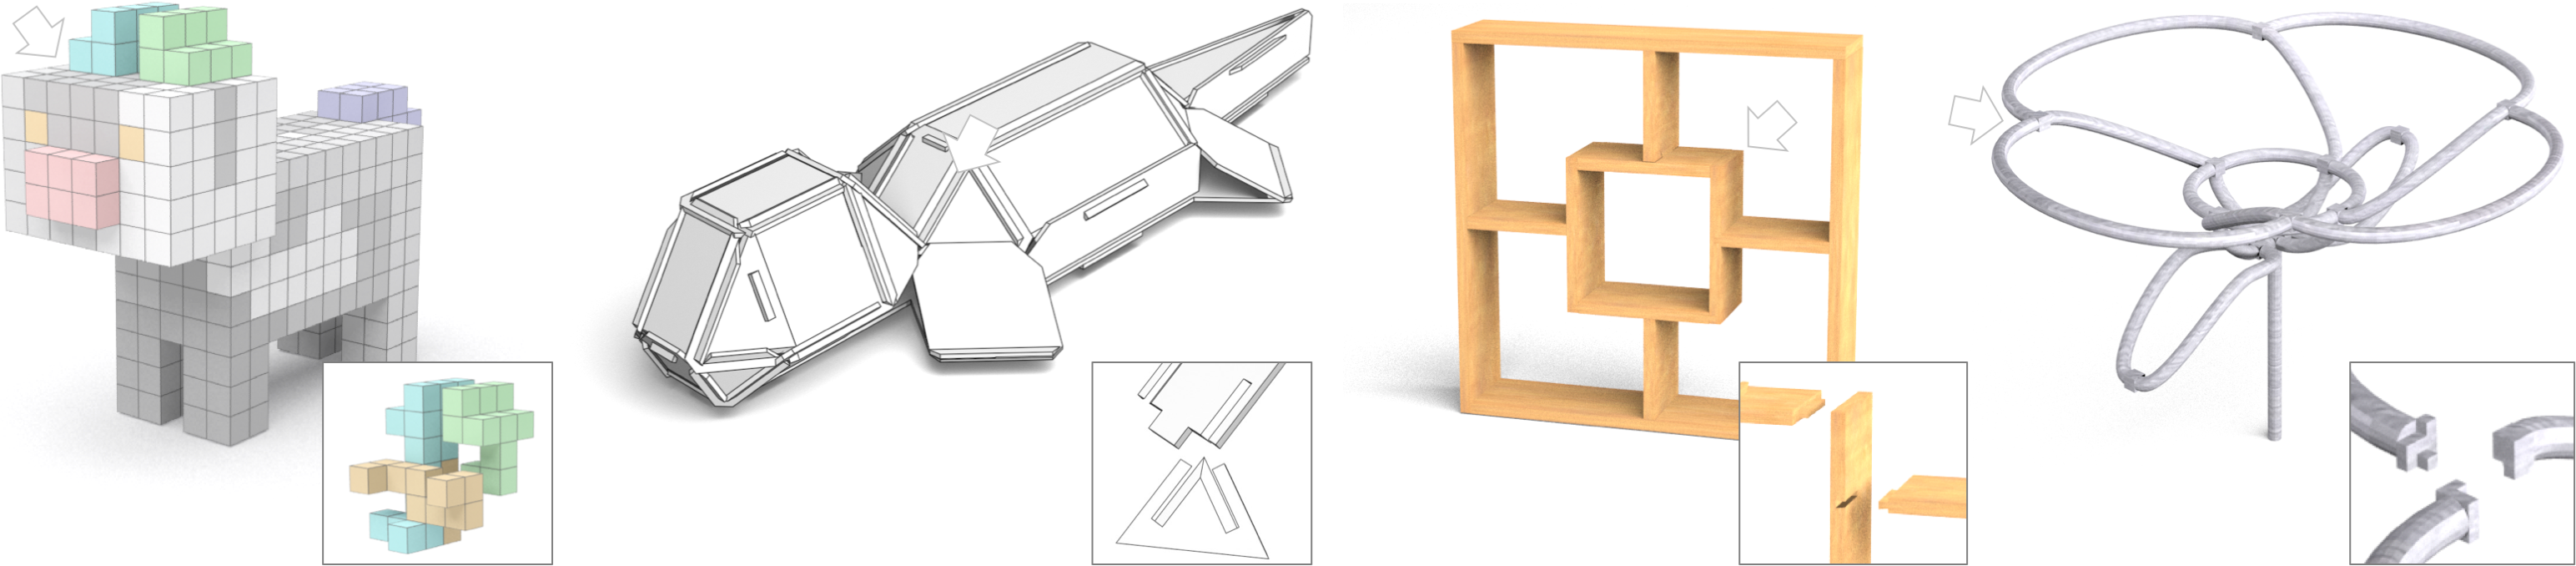
\includegraphics[width=\textwidth]{images/Teaser.png}
%	\caption{Various interlocking assemblies designed using our framework, from left to right: voxelized puzzle, plate structure, furniture, and frame structure. Our method supports different types of joints as highlighted in the zooms. Please refer to the accompanying video for assembly sequences and the supplementary material for the blocking graphs defining the interlocking configurations.}
%	\label{fig:teaser}
%	\vspace*{1.5mm}
%\end{teaserfigure}

\input{Section0-abstract} 


\if 0
%CCS
\begin{CCSXML}
<ccs2012>
<concept>
<concept_id>10010147.10010371.10010372</concept_id>
<concept_desc>Computing methodologies~Rendering</concept_desc>
<concept_significance>500</concept_significance>
</concept>
<concept>
<concept_id>10010147.10010371.10010372.10010374</concept_id>
<concept_desc>Computing methodologies~Ray tracing</concept_desc>
<concept_significance>500</concept_significance>
</concept>
</ccs2012>
\end{CCSXML}

\ccsdesc[500]{Computing methodologies~Rendering}
\ccsdesc[500]{Computing methodologies~Ray tracing}

%keywords
\keywords{ray tracing, global illumination, octrees, quadtrees}
\fi


% Processes all of the front-end information and starts the body of the work.
\maketitle



%%%%%%%%%%%%%%%%%%%%%%%%%%%%%%%%%%%%%%%%%%%%%%%%%%%%%%%%%%%%%%%%%%%%%%%%%%%%%


%%%%%%%%%%%%%%%%%%%%%%%%%%%%%%%%%%%%%%%%%%%%%%%%%%%%%%%%%%%%%%%%%%%%
% Introduction
%%%%%%%%%%%%%%%%%%%%%%%%%%%%%%%%%%%%%%%%%%%%%%%%%%%%%%%%%%%%%%%%%%%%

\section{Introduction}
\label{sec:introduction}

% 3D assemblies: parts connection
3D assemblies refer to objects that combine multiple component parts into a structure with a specific form and/or functionality.  Connection mechanisms are usually required to prevent the parts from moving relative to one another and make the assembly steady for practical usage.
However, these connectors can be irreversible (e.g., glue), impair the structural integrity of parts (e.g., nails), or degrade the external appearance of the assembly (e.g., clamps).
%In addition, connecting parts with these fasteners could be a tedious task, e.g., gluing two parts together requires aligning the parts accurately.

% 3D interlocking assemblies: properties and applications
Rather than relying on additional explicit connectors, interlocking assemblies connect parts into a steady structure  based only on the geometric arrangement of the parts. This intriguing property facilitates repeated assembly and disassembly and significantly simplifies the correct alignment of parts during construction.
Consequently, interlocking assemblies have been used in a variety of applications, including puzzles~\cite{Stegmann-2018-PuzzlePage}, furniture~\cite{Fu-2015-Furniture}, architecture~\cite{Deepak-2012-InterlockBlock}, and 3D printing~\cite{Yao-2017-InterlockShell}.

% Designing 3D interlocking assemblies
In an interlocking assembly, parts need to follow certain orders to be assembled into the target object.
Once assembled, there is only one movable part, called the {\em key},  while all other parts as well as any subset of  parts are immobilized relative to one another~\cite{Song-2012-InterCubes}.
However, this defining property of parts immobilization makes designing interlocking assemblies highly challenging. Explicitly testing the immobilization of every subset of parts requires costly computations; optimizing for the geometry of parts that satisfy these immobilization requirements, while avoiding dead-locking, is even more complex.
%Second, modifying an individual part could easily break the global interlocking property.
%Second, the parts still can be disassembled without deadlocking.

% Limitations of existing approaches
Recently, several computational approaches have been developed to address this problem~\cite{Xin-2011-BurrPuzzles, Song-2012-InterCubes, Fu-2015-Furniture, Song-2016-CoFiFab, Zhang-2016-InterlockVoxel, Song-2017-ReconfigInterlock, Yao-2017-InterlockShell}.
The common idea is to directly guarantee global interlocking by constructing and connecting multiple local interlocking groups (LIGs), which avoids the overhead of testing all part subsets for immobilization.
While these methods show successful results, they only focus on specific sub-classes of interlocking assemblies, e.g., recursive interlocking puzzles ~\cite{Song-2012-InterCubes}, but do not explore the full search space of all possible interlocking configurations.
As a consequence, these approaches are restricted in the kind of input shapes they can handle and  have limited flexibility to satisfy additional design requirements besides interlocking, e.g., related to aesthetics or functional performance.

%Hence, these approaches are quite restrictive in three aspects.
%First, they actually focus on a special subset of general interlocking assemblies, e.g., recursive interlocking puzzles by~\cite{Song-2012-InterCubes}.
%First, these approaches can only handle input shapes that satisfy certain requirements, e.g., \cite{Fu-2015-Furniture} requires the input furniture has many small cyclic substructures.
%Second, their interlocking designs are difficult to be edited and reused since slight modification on these designs could break the carefully achieved global interlocking, while existing approaches have no way to correct these modifications.

% Our focus: general interlocking assembly
%The above limitations arise because existing approaches keep using a similar divide-and-conquer strategy  for the purpose of generating specific interlocking designs while do not fully explore the all possible interlocking configurations.
\pagebreak

\vspace*{2.0mm}
\noindent
{\bf Contributions.} \
In this paper, we propose a new general framework for DESigning Interlocking Assemblies, called {\em DESIA}, that avoids the restrictions of previous LIG-based methods.
Specifically, we make the following  contributions:


%we investigate the mechanism of interlocking assemblies in greater depth, aiming at developing a general computational method for designing interlocking assemblies.
%In particular, we focus on  3D assemblies that have rigid parts and neighboring parts have planar surface contact such that each part can only have translational motion (i.e., no rotational motion) in the final assembly.

% Our contributions:
%The paper makes the following contributions:

%\vspace*{-1.0mm}
\begin{itemize}[leftmargin=*]
\item 
We represent interlocking assemblies with a set of base {\em Directional Blocking Graphs} (DBGs) and implement an efficient graph analysis algorithm that can test for global interlocking in polynomial time complexity.

%We connect interlocking assemblies with the {\em Non-Directional Blocking Graph} (NDBG)~\cite{Wilson-1992-AssemblyPlanning} that describes parts blocking relations in an assembly, and check interlocking with polynomial time complexity by taking advantage of the graphs.

%We formulate interlocking property of general 3D assemblies as a set of mathematical inequalities.
%This formulation leads to an intuitive graph-based \Mark{give a name to the graph} representation of interlocking assemblies, where each directed graph represents the parts immobilization relationship along a specific part movable direction. \Peng{need to compare with~\cite{Tai-2012-InterlockRF,Wilson-1992-AssemblyPlanning}}
%We show that an assembly is interlocking if each directed graph forms a single strongly connected component, without considering the key 
%assuming the key is held by some other means.

\vspace*{1.0mm}
\item  
We introduce a general iterative framework for designing interlocking assemblies that can explore the full search space of all possible interlocking configurations by utilizing existing part blocking relations described in the graphs.

\vspace*{1.0mm}
\item We demonstrate the flexibility of our framework for designing different classes of assemblies, including new types of interlocking forms that have not been explored in previous works.

 \end{itemize}

\noindent
%Directional blocking graphs were first proposed in the context of mechanical assemblies by Wilson~\shortcite{Wilson-1992-AssemblyPlanning} to describe part relations. In our work we show that a small set of base DBGs is ideally suited to encode mutual blocking relations for interlocking assemblies.

%Our method allows identifying certain kinds of input models (with known parts-graph) that cannot be interlocking, no matter what kinds of joints are created among the parts, and provides suggestions to modify these input models to enable interlocking. 




%The key idea is to compute local blocking relations among parts that are required for achieving global interlocking by maintaining a dynamic NDBG, and constructe parts/joints geometry to realize these local blocking relations.  

%This cannot be achieved by previous approaches that focus on each specific kind of interlocking assemblies.



%\vspace*{1.5mm}
%\item 
%We also prove the formal models in previous works~\cite{Song-2012-InterCubes,Fu-2015-Furniture} that directly guarantee global interlocking. 
%\Mark{better to put this in the conclusion}


The rest of the paper is organized as follows. We first discuss related work in Section~\ref{sec:related}.
In Section~\ref{sec:model} we introduce our graph-based representation for assemblies and present an efficient algorithm for testing whether an assembly is interlocking. Section~\ref{sec:approach} then describes our computational framework for designing interlocking assemblies.
In Section~\ref{sec:results} we show different types of assemblies generated with our approach, compare with previous works, and highlight several application examples.  We conclude with a discussion of limitations of our approach and some thoughts on future research problems.


\if 0
We demonstrate that our general framework allows generating new interlocking assemblies of various forms, has more flexibility to design interlocking assemblies than previous approaches, and supports editing existing interlocking assemblies according to a user's design intent. 
In particular, a new kind of interlocking assemblies has been successfully designed using our framework, which is an interlocking frame with elongated rods connected by voxelized joints. \Mark{Not sure if we want to highlight this here.}
We also realized our designed assemblies with LEGO bricks and 3D printing, and demonstrated that their steadiness is comparable with that from previous approaches~\cite{Song-2012-InterCubes, Fu-2015-Furniture}.
\fi

% Our experiments and results





% our focus: understand the govering mechanism of interlocking assemblies and develop more flexible and powerful constructive methods to design new interlocking assemblies that are interlocking only at the final assembled state
% assumption:
% - only translation,
% -  surface contact among neighboring parts
% may need an exmaple to say that recurisve interlocking is not a must




% since it is difficult to directly gurantee the gloal interlocking property, divide-and-conquer, local interlocking -> global interlocking
% avoid the exponential complexity of checking global interlocking property for (assembly with a large number of parts)
%  -  assembly order is quite fixed (enhance stability during parts assembly)
% reason: do not fully understand the mechanism of 3D interlocking






% our experiments


%%%%%%%%%%%%%%%%%%%%%%%%%%%%%%%%%%%%%%%%%%%%%%%%%%%%%%%%%%%%%%%%%%%%%%%%%%%%%%
% Backup
%%%%%%%%%%%%%%%%%%%%%%%%%%%%%%%%%%%%%%%%%%%%%%%%%%%%%%%%%%%%%%%%%%%%%%%%%%%%%%







%
%%%%%%%%%%%%%%%%%%%%%%%%%%%%%%%%%%%%%%%%%%%%%%%%%%%%%%%%%%%%%%%%%%%%
% Related work
%%%%%%%%%%%%%%%%%%%%%%%%%%%%%%%%%%%%%%%%%%%%%%%%%%%%%%%%%%%%%%%%%%%%

%\vspace*{-2.0mm}
\section{Related Work}
\label{sec:related}


%%%%%%%%%%%%%%%%%%%%%%%%%%%%%%%%%%%%%%%%%
% 1. Connecting Parts in 3D Assemblies
%%%%%%%%%%%%%%%%%%%%%%%%%%%%%%%%%%%%%%%%%

\vspace*{2.0mm}
\noindent
{\bf Connecting Parts in 3D Assemblies.}  \
%Large and/or complex objects, such as architecture, are usually fabricated with parts rather than a single piece.
%This not only reduces the fabrication cost by using simpler parts, but also facilitate the maintenance since broken parts can be easily replaced \Mark{claim less about the maintenance; better to put it as a future work}.
To create a multi-part object for practical use,  component parts need to be assembled and tightly connected.
For example, glue is used to connect 3D printed parts~\cite{Chen-2015-Dapper,Vanek-2014-PackMerger, Hu-2014-Pyramidal}
although glued parts cannot be separated easily, discouraging parts disassembly and reassembly.
% and its connection strength is highly dependent on the part material.
Nails and screws are commonly used in furniture~\cite{Shao-2016-Furniture,Lau-2011-Furniture}.
% and laser-cut objects~\cite{Weichel-2012-Enclosed}.
However, these fasteners may break the parts and become loose after repeated disassembly and reassembly.
Wire also can be used for  part connections~\cite{Attene-2015-ShapesInABox, Richter-2015-BeamMeshes}, yet tying parts together could be a tedious task.

\begin{figure}[!b]
	\centering
	\vspace*{-4.0mm}
	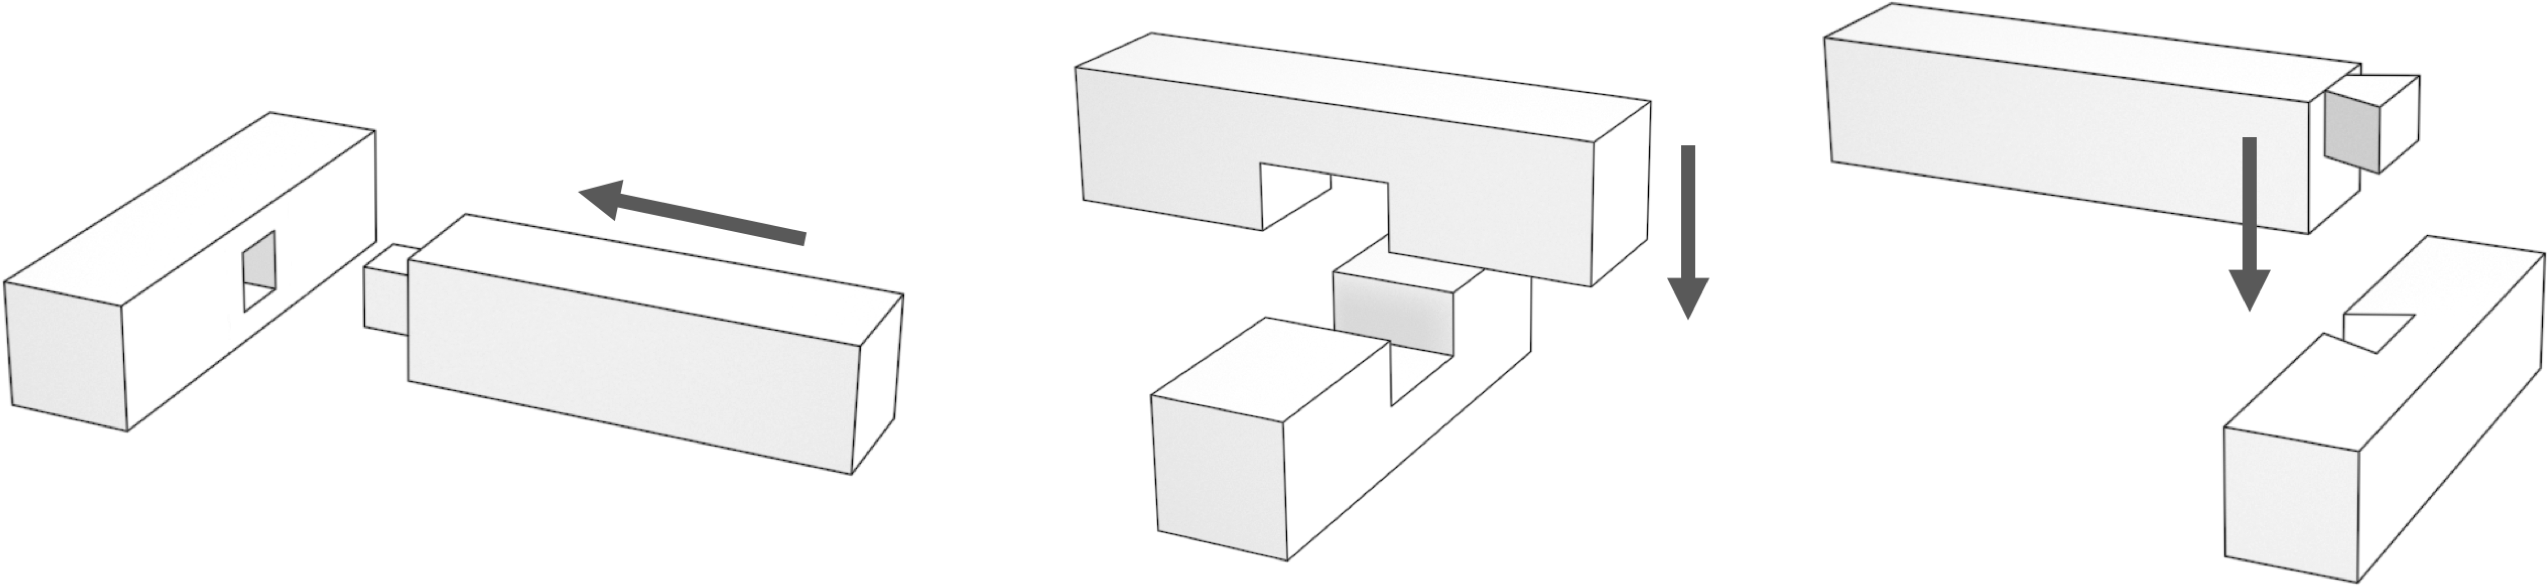
\includegraphics[width=8.00cm]{images/Joints.png}
	\vspace*{-2.5mm}
	\caption{Example woodworking joints. From left to right: mortise-and-tenon, halved joint, and dovetail joint, where the black arrow shows the single part movable direction allowed by the joint.}
	%\vspace*{-4.0mm}
	\label{fig:Joints}
\end{figure}


In practice, integral joints are often preferred for connecting parts, since they greatly simplify the assembly process. For example, woodworking joints (see Figure~\ref{fig:Joints}) are widely used in furniture design~\cite{Yao-2017-DecorativeJoinery,Koo-2017-ZeroWaste,Chen-2015-FreshPressModeler,Schwartzburg-2013-PlanarPieces},
mortise-and-tenon joints for 3D printed object assemblies~\cite{Luo-2012-Chopper, Hao-2011-PartitionModels, Duncan-2016-Hands-OnAssembly}, and
halved joints for laser-cut shape abstractions~\cite{Cignoni-2014-MeshJoinery,  Hildebrand-2012-crdbrd,McCrae-2011-Slices}.
However, these joints only constrain relative part motion locally, and the resulting assembly typically relies on other means, e.g., friction and/or gravity, to lock the parts in place.
%\Mark{add a figure to show various parts connection methods}

%%%%%%%%%%%%%%%%%%%%%%%%%%%%%%%%%%%%%%%%%
% 2. Self-supporting Structures
%%%%%%%%%%%%%%%%%%%%%%%%%%%%%%%%%%%%%%%%%

\vspace*{2.0mm}
\noindent
{\bf Self-supporting Structures},  
e.g., masonry buildings~\cite{Rippmann-2016-ArmadilloVault} and puzzles~\cite{Frick-2015-Self-SupportPuzzle}, are assemblies of rigid components that do not require any binder to connect the parts. The entire structure is in static equilibrium through gravity-induced compression forces that immobilize all the parts~\cite{Whiting-2009-ModelMasonry}.
%
Recently, the design of freeform self-supporting structures has  received a lot of interest in computer graphics.
Some research works focus on designing 3D surfaces that only exhibit internal compression forces under gravity~\cite{Miki-2015-AiryStressFunctions,Tang-2014-PolyhedralMesh,Liu-2013-RegularTriangulation,deGoes-2013-Equilibrium,Vouga-2012-Self-SupportSurface},
while others focus on the design, fabrication, and assembly of self-supporting structures~\cite{Rippmann-2016-ArmadilloVault,Deuss-2014-AssembleSelfSupport,Panozzo-2013-SelfSupportMasonry}.  
%
Self-supporting structures can only bear compression load but are not designed to handle any tensile forces.
This is reasonable for certain architectural structures that are built to bear their own weight, but not for general spatial assemblies that experience forces in arbitrary directions. The strategy of immobilizing parts in self-supporting structures is therefore not applicable in our general assembly setting.

%In particular, Panozzo et al.~\shortcite{Panozzo-2013-SelfSupportMasonry} designed and fabricated unreinforced masonry models consisting of hexagonal blocks while
%Deuss et al.~\shortcite{Deuss-2014-AssembleSelfSupport} constructed freeform self-supporting structures by using a sparse set of chains connected to fixed anchor points.




%%%%%%%%%%%%%%%%%%%%%%%%%%%%%%%%%%%%%%%%%
% 3. Interlocking Assemblies
%%%%%%%%%%%%%%%%%%%%%%%%%%%%%%%%%%%%%%%%%

\vspace*{2.0mm}
\noindent
{\bf Interlocking Assemblies.} \ 
Several computational methods have recently been developed to construct interlocking assemblies. 
Xin et al.~\shortcite{Xin-2011-BurrPuzzles} create 3D interlocking puzzles by replicating and connecting multiple instances of a six-piece interlocking burr structure. 
Rather than reusing an existing structure,  Song et al. ~\shortcite{Song-2012-InterCubes} construct 3D interlocking
puzzles by iteratively extracting pieces from a voxelized 3D shape and enforcing a local interlocking condition among every three consecutive pieces. 
Song et al.~\shortcite{Song-2015-Interlock} extend this method to handle smooth non-voxelized shapes for 3D printing.
Zhang and Balkcom~\shortcite{Zhang-2016-InterlockVoxel} define a set of voxel-like interlocking blocks and connect instances of these blocks layer-by-layer into various voxelized shapes. 

Different from above works that take a 3D solid object as an input, Fu et al.~\shortcite{Fu-2015-Furniture} focus on frame-based structures such as furniture that have been initially partitioned into parts. They compute an interlocking joint configuration by planning and connecting local interlocking groups.
This method has been extended to interlock 2D laser-cut parts into a convex polyhedron~\cite{Song-2016-CoFiFab} and to design reconfigurable furniture with multi-key interlocking~\cite{Song-2017-ReconfigInterlock}.
Yao et al.~\shortcite{Yao-2017-InterlockShell} design and optimize interlocking shell pieces for 3D printing. They employ 3D simulation to test whether the resulting shell assemblies are interlocking.
However, this generate-and-test paradigm is relatively inefficient and applicable only for assemblies with a small number of interlocking pieces.

The key idea of the above works (except~\cite{Yao-2017-InterlockShell}) is to design interlocking assemblies by constructing and connecting multiple local interlocking groups.  
This strategy skillfully avoids the global test for interlocking of the resulting assemblies, which would have a time complexity that is exponential in the number of parts~\cite{Song-2012-InterCubes}. 
While this strategy allows designing interlocking assemblies with many parts, the search space is restricted to a small subset of all possible interlocking configurations.
Our experimental results in Section~\ref{sec:results}  show that the flexibility of designing interlocking assemblies can be significantly increased by our method's ability to explore the full search space.
%indicate that this restricted subset is indeed very small, and
%\Mark{need to show why the small subset is not good or to show the goodness of interlocking configurations that are out of the subset.}

\if 0
Compared with above works that focus on each specific kind of interlocking assemblies, this work studies the common governing mechanics of interlocking assemblies that may have different forms and develops a general constructive approach for designing these assemblies.
In particular, this work builds connections between interlocking assemblies and the NDBG~\cite{Wilson-1992-AssemblyPlanning}, making it possible to take advantage of existing graph theory and algorithms to explore the full search space of interlocking configurations. 
%This not only leads to an approach that can test interlocking with polynomial time complexity, 
\fi



%%%%%%%%%%%%%%%%%%%%%%%%%%%%%%%%%%%%%%%%%
% 4. Assembly Planning
%%%%%%%%%%%%%%%%%%%%%%%%%%%%%%%%%%%%%%%%%

\vspace*{2.0mm}
\noindent
{\bf Assembly Planning} \
is the problem of finding a sequence of motions to assemble a structure from its parts. 
This problem has been extensively studied in robotics and we refer to~\cite{Ghandi-2015-AssemblyPlanningReview} for a thorough review.
Assembly planning is also relevant for computer graphics applications, e.g., for generating visual assembly instructions~\cite{Agrawala-2003-AssemblyInstructions,Guo-2013-IllustrateDisassembly} or creating exploded view diagrams~\cite{Li-2008-ExplodedView}.

Finding an assembly plan requires identifying movable parts and part groups at each stage of the assembly, often leading to a combinatorial search problem.
To solve this task more efficiently, Wilson~\shortcite{Wilson-1992-AssemblyPlanning} invented a {\em Directional Blocking Graph} and a {\em Non-Directional Blocking Graph} to represent blocking relations among parts in an assembly. 
Tai~\shortcite{Tai-2012-InterlockRF} employed these graphs for designing reciprocal frames connected with notched joints, aiming at minimizing the number of movable parts and part groups in the final assembly.
%\Mark{good to cite some works outside of computer graphics community;
%	we focus on designing parts geometry while above works focus on "designing" (dis)assembly sequences }
Rather than focusing on assembly planning, our work, to the best of our knowledge, is the first to employ these graphs for computational design of interlocking assemblies. 
% parts and/or joints geometry construction for designing new interlocking assemblies.




\if 0
, Wilson and Latombe~\shortcite{Wilson-1994-GeometricReasoning} developed a {\em Directional Blocking Graph} (DBG)  to represent blocking relations among parts in an assembly along a certain translational direction and summarized all these graphs for all possible translational directions to construct a {\em non-directional blocking graph} (NDBG).
The NDBG allows to address the combinatorial problem of automatically computing the assembly sequences of a 3D assembly in polynomial time complexity of the number of parts involved. 
Tai~\shortcite{Tai-2012-InterlockRF}  presented a computational approach to construct wooden frames connected with notched joints.
They search  joint configurations using a  genetic algorithm to find wooden frame that is disassemblable and leans towards being global interlocking.
Directional Blocking Graph (DBG) is employed to identify all movable parts or part groups in the assembly to analyze the interlocking condition.
\fi





%\newpage







%%%%%%%%%%%%%%%%%%%%%%%%%%%%%%%%%%%%%%%%%%%%%%%%%%%%%%%%%%%%%%%%%%%%%%%%%%%%%%
% Backup
%%%%%%%%%%%%%%%%%%%%%%%%%%%%%%%%%%%%%%%%%%%%%%%%%%%%%%%%%%%%%%%%%%%%%%%%%%%%%%






%%%%%%%%%%%%%%%%%%%%%%%%%%%%%%%%%%%%%%%%%%%%%%%%%%%%%%%%%%%%%%%%%%%%%
% Overivew
%%%%%%%%%%%%%%%%%%%%%%%%%%%%%%%%%%%%%%%%%%%%%%%%%%%%%%%%%%%%%%%%%%%%

\section{Model Interlocking Assemblies}
\label{sec:model}



In this section, we introduce our conceptual representation of interlocking assemblies using a family of directed graphs. We show how this graph-based representation leads to an efficient algorithm to {\em test} interlocking. 
In Section~\ref{sec:approach} we then explain how to effectively employ this representation and algorithm to {\em design} interlocking assemblies.
%\TODO{one more assumption: we focus on (dis)assemblies parts with translational motions, e.g., do not consider taking a part by rotating it first and then doing the translation.}


\begin{figure}[!t]
	\centering
	%\vspace*{-3.5mm}
	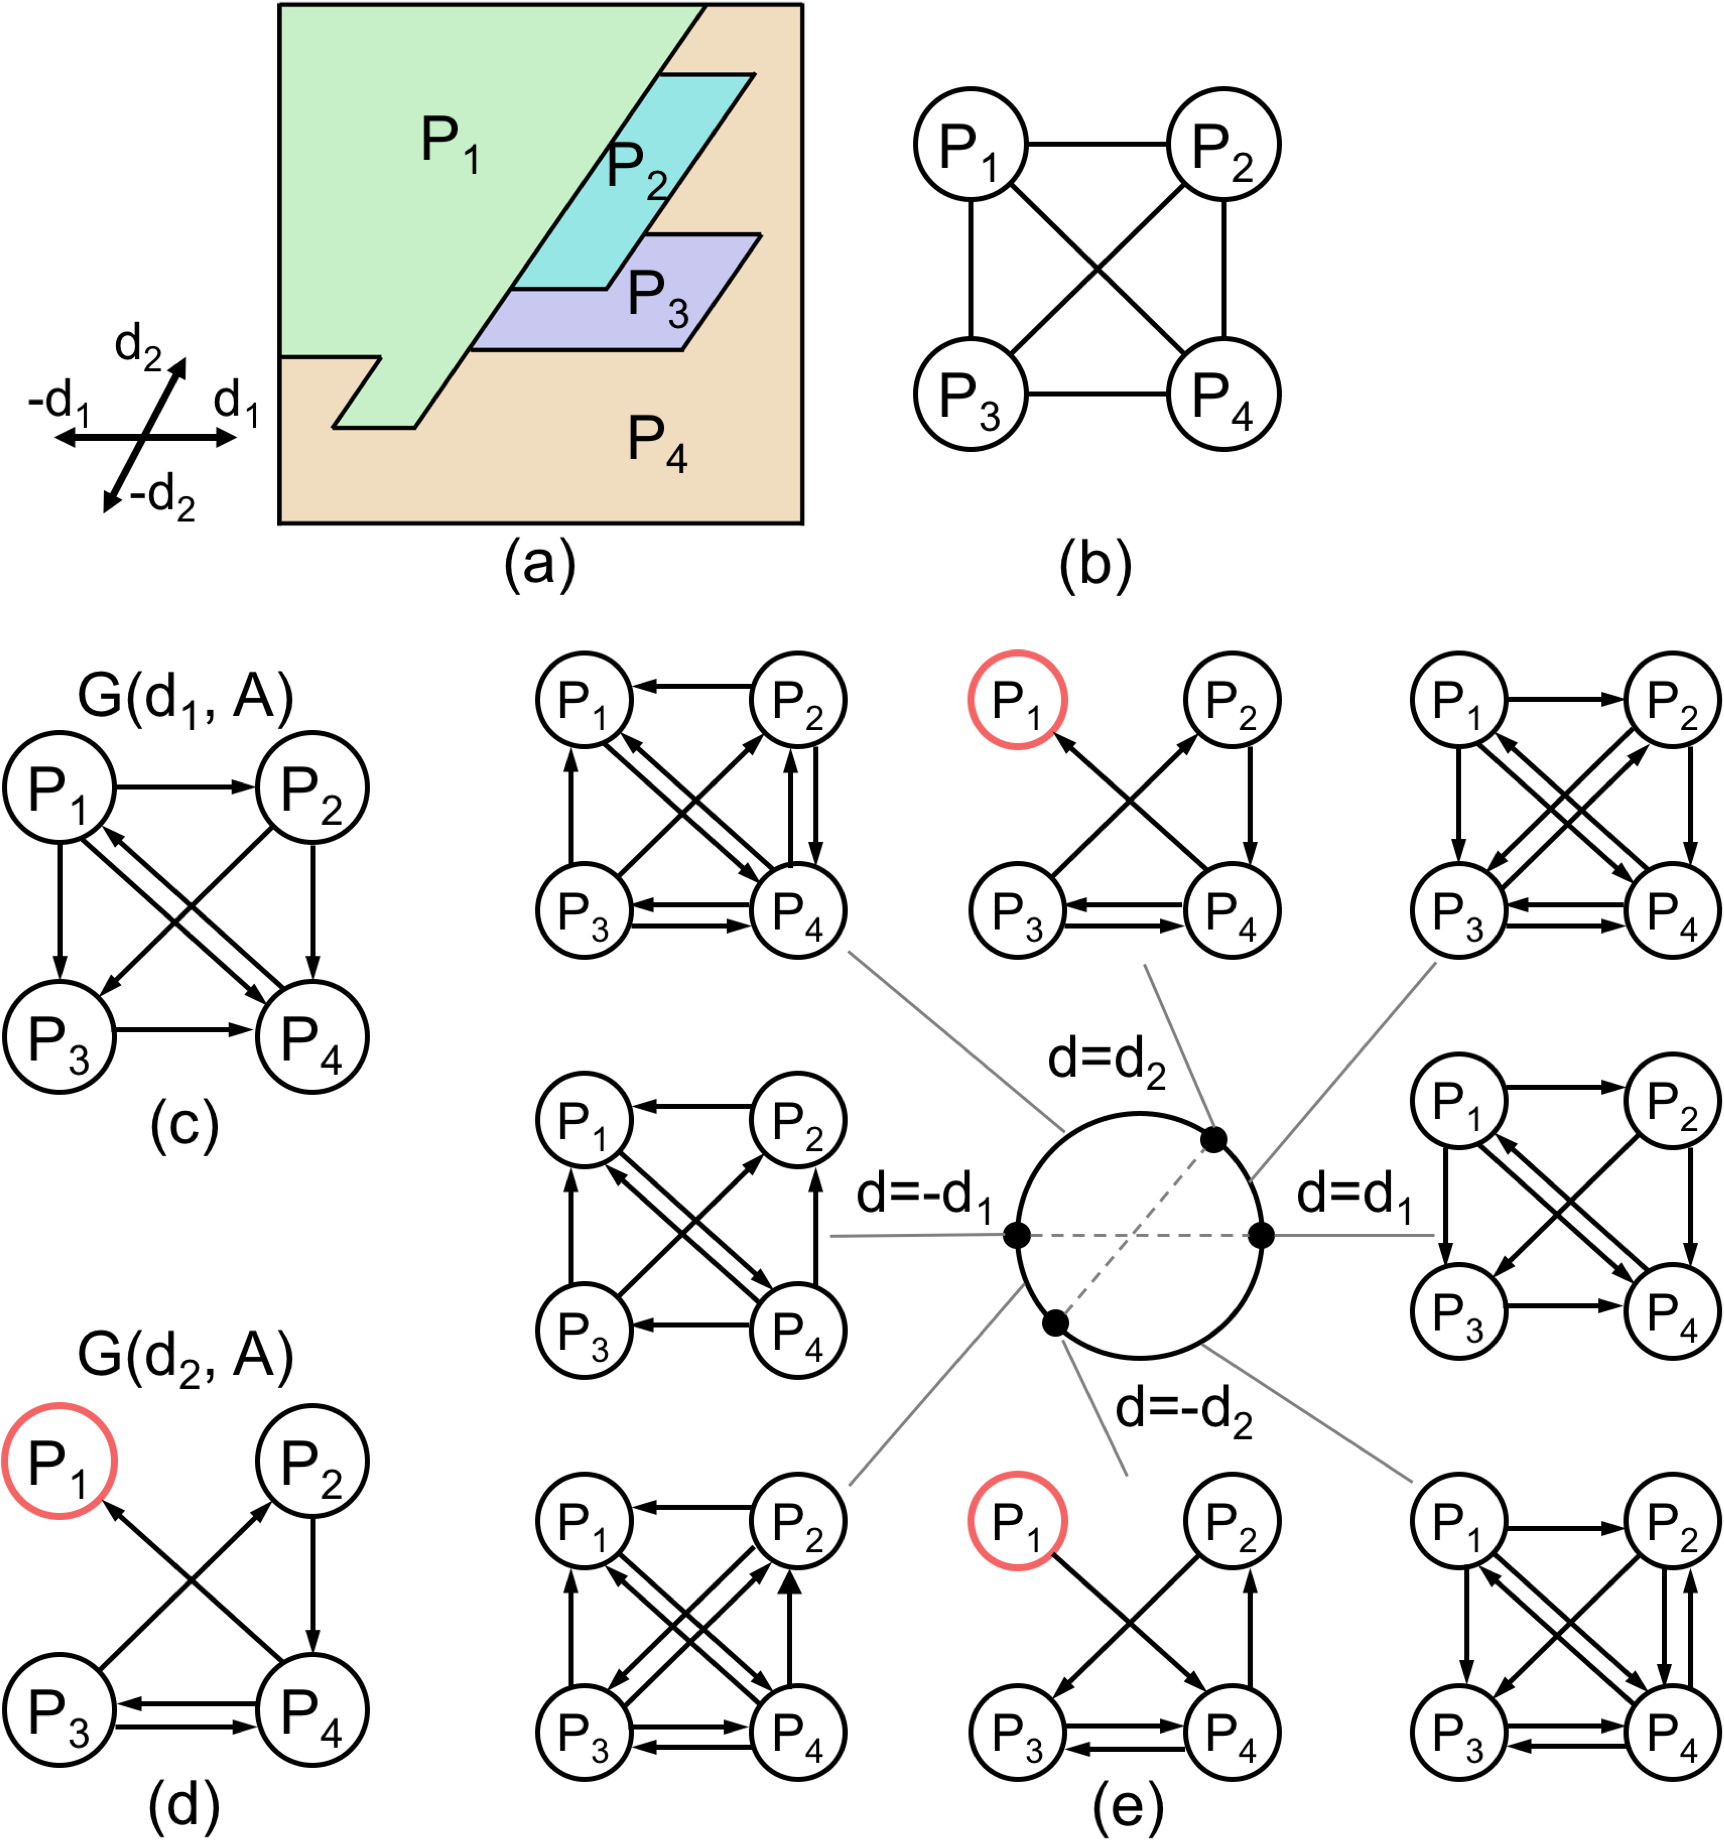
\includegraphics[width=8.00cm]{images/NDBG.png}
	\vspace*{-2.5mm}
	\caption{Example DBGs and NDBG.
		(a\&b) A 2D interlocking assembly and its parts-graph, where the key $P_1$ is movable along $d_2$;
		(c\&d) Two DBGs of the assembly; and
		(e) NDBG of the assembly.
		A part with zero out-degree or in-degree in a DBG is highlighted with a red circle. 
		%\Mark{I would still consider using crossing edges, I think it will make it easier to read.I would also expand the figure  to reach to full width, i.e. add more space.}
	}
	\vspace*{-4.0mm}
	\label{fig:NDBG}
\end{figure}



\subsection{Graph Model}

%%%%%%%%%%%%%%%%%%%%%%%%%%%%%%%%%%%%%%%%%%%%%%%%
% Our Inputs
%%%%%%%%%%%%%%%%%%%%%%%%%%%%%%%%%%%%%%%%%%%%%%%%

Consider an assembly $\mathbf{A}$, made of $n$ parts $P_1$, $...$, $P_n$.
We make the following assumptions:
1) each part $P_i$ is rigid; 
2) neighboring parts have planar surface contact only; and 
%(e.g., corner-surface and edge-surface contacts are not considered); and
3) $\mathbf{A}$ can be disassembled by single-part translational motions, i.e., part rotation is not required and all other parts remain fixed when removing a part.


%%%%%%%%%%%%%%%%%%%%%%%%%%%%%%%%%%%%%%%%%%%%%%%%
% Base DBGs
%%%%%%%%%%%%%%%%%%%%%%%%%%%%%%%%%%%%%%%%%%%%%%%%

\vspace*{1.0mm}
\noindent
{\bf Directional Blocking Graph (DBG).}\  
We denote as $G(d, A)$ the {\em directional blocking graph} of assembly $\mathbf{A}$ for translation along direction $d$. 
This directed graph has nodes representing the parts of $\mathbf{A}$ and directed edges $e_{i \rightarrow j}$ from $P_i$ to $P_j$  if and only if $P_j$ prevents any translational motion of $P_i$ along $d$. 
In other words, $e_{i \rightarrow j}$ can be read as ``$P_i$  is blocked by $P_j$" in direction $d$. 
See Figure~\ref{fig:NDBG}(c\&d) for two examples.

If $G(d, A)$ is {\em strongly connected}, i.e. if every node can be reached from every other node, no part or part group is movable along $d$; see Figure~\ref{fig:NDBG}(c). 
A part group $\mathbf{S}$ of $\mathbf{A}$ is locally free to translate in direction $d$ ($-d$), if and only if the out-degree (in-degree) of $\mathbf{S}$ in $G(d, A)$ is zero; see $P_1$ in Figure~\ref{fig:NDBG}(d).
%there is no edge in $G(d, A)$ connecting parts in $\mathbf{S}$ to parts in $\mathbf{A} \setminus \mathbf{S}$; see $P_1$ in Figure~\ref{fig:NDBG}(d) for an example.
%since there is no out-edge connecting it with the other nodes in the graph; see Figure~\ref{fig:NDBG}(d). 

\begin{figure*}[!t]
	\centering
	%\vspace*{-3.5mm}
	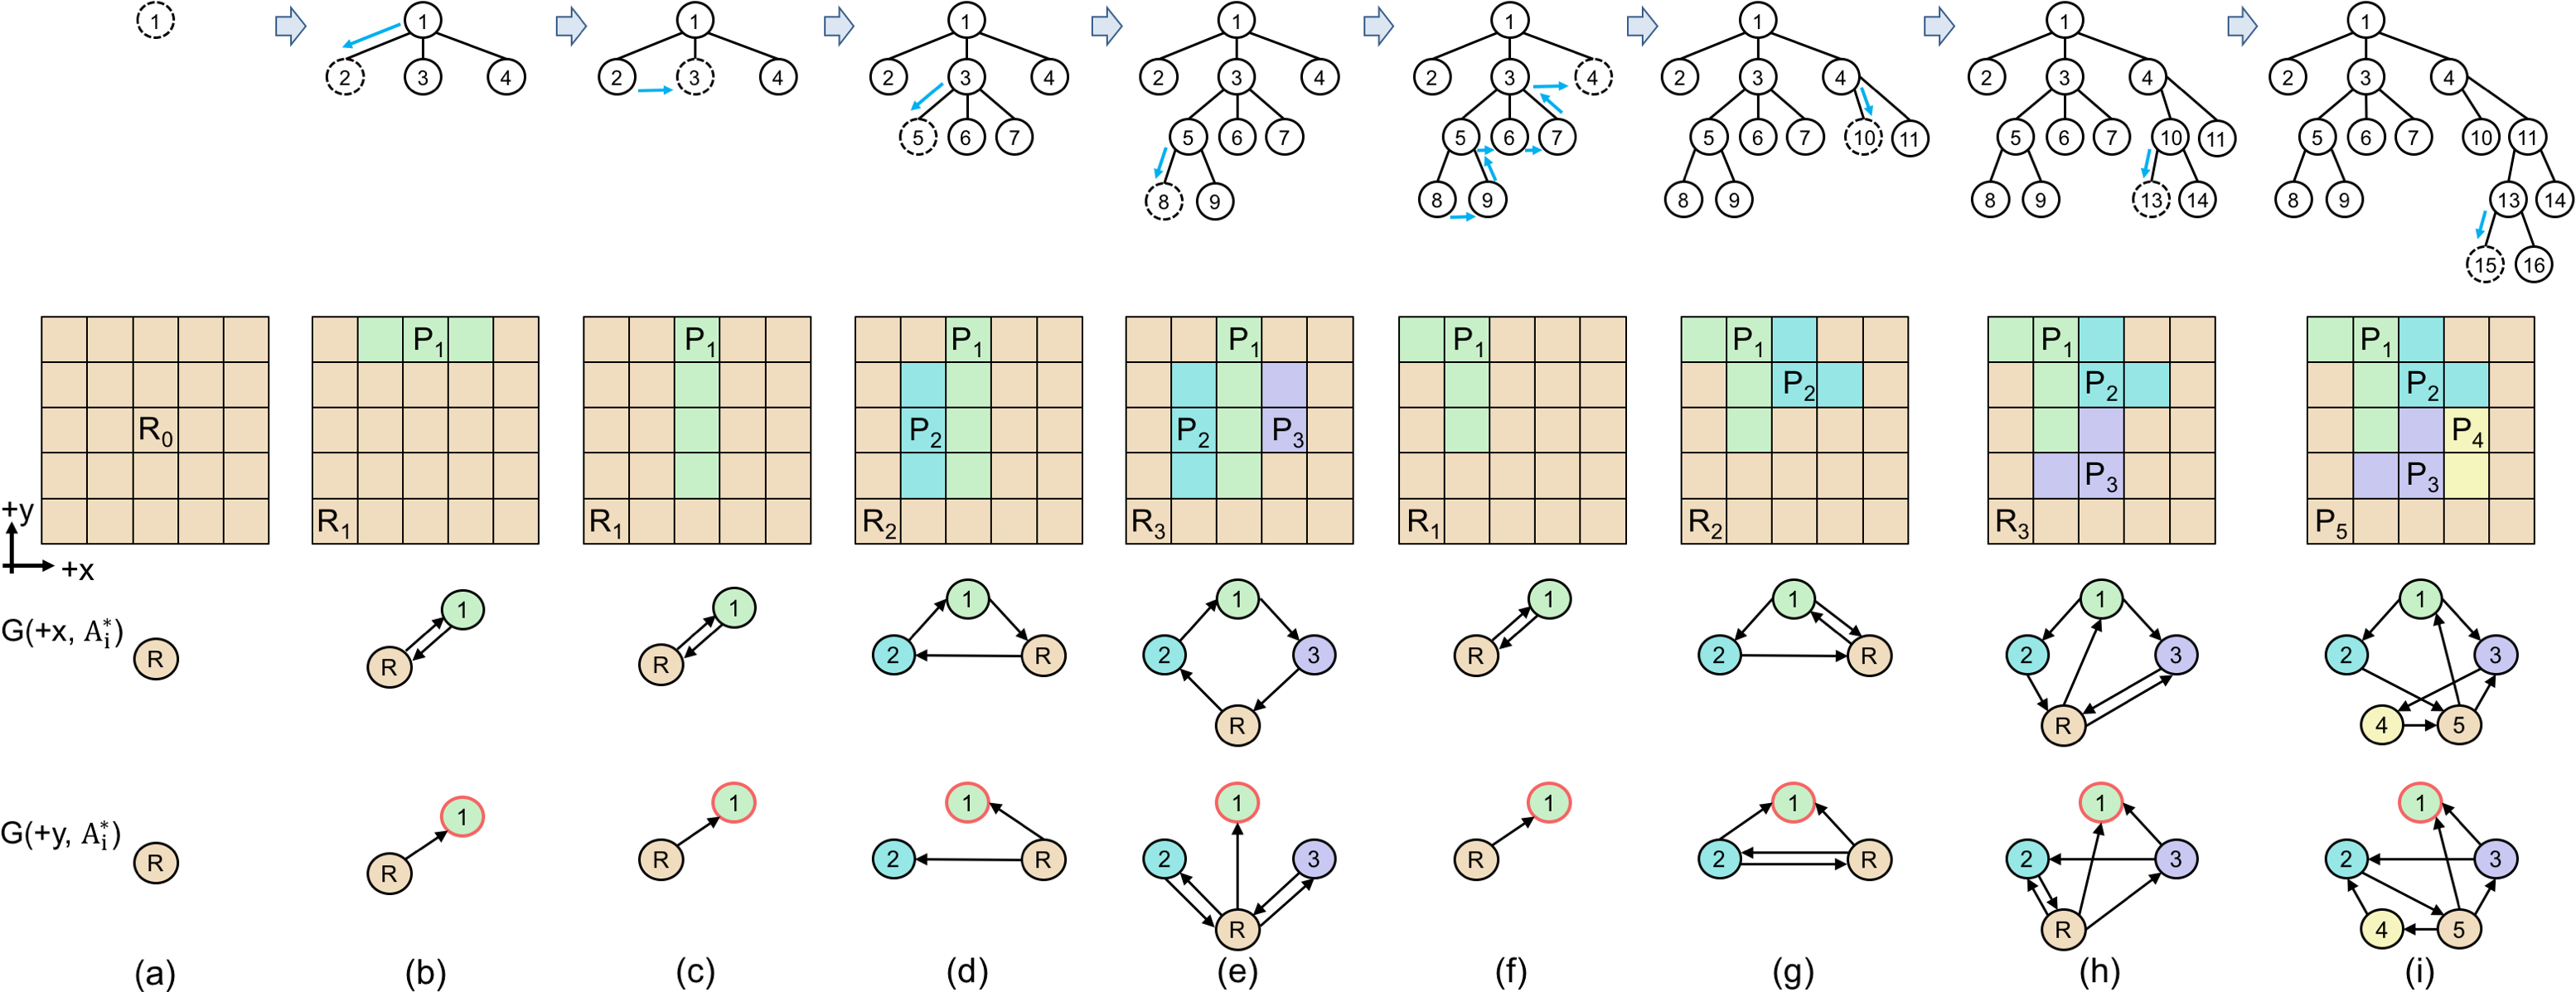
\includegraphics[width=17.80cm]{images/Framework_Overview.png}
	\vspace*{-2.5mm}
	\caption{		
		Overview of our framework on a 2D interlocking design.
		(a) Given a $5 \times 5$ square as input, (b-i) our framework tries to generate a 5-part interlocking 2D assembly, in which each part should have at least two pixels.
		Top row: Construction tree, where each node at depth $i$ represents a candidate of $\mathbf{A}_i$.
		%Each node can have at most $M=3$ children, and the leftmost child in the tree has the highest ranking.
		Here we show the $M=3$ highest ranked options at each level with the top-ranked on the left.
		%\Mark{Maybe better "Here we show the $M=3$  highest ranked options with the top-ranked on the left." We don't want to imply that $M=3$ is some fixed threshold.}		
		The blue arrows indicate the procedure to visit the nodes for generating parts. 
		If the framework cannot find any child for the current node (in dashed circle, denoted as $\mathbf{A}_i^*$), it will backtrack to (c) its siblings or (f) ancestors.
		Middle row: Geometric examples corresponding to the dashed node in the tree.
		Bottom row: Base DBGs of the geometric examples, where the key is indicated by a red circle. For simplicity, we show nodes $P_j$ ($j\leq i$)  as $j$, and $R_i$ as $R$.
		%\Mark{I would add more vertical spacing between the rows.}
	\vspace*{-3.0mm}
	\label{fig:Framework_Overview}}
\end{figure*}


\vspace*{1.0mm}
\noindent
{\bf Non-directional Blocking Graph (NDBG).} \
We represent the set of all translation directions in 2D by the unit circle denoted as $C$.
For every pair of parts in contact in $\mathbf{A}$, we draw the diameter that is parallel with the contact line.
The drawn diameters partition $C$ into an arrangement of regions, for which the corresponding DBG $G(d, A)$ remains constant when $d$ varies over a region.
For any pair of parts in 
%\vspace*{-1mm}
\setlength{\columnsep}{13pt}
\begin{wrapfigure}{r}{0.32\columnwidth}
	\vspace{-6pt}
	\centering
	\hspace{-4pt}
	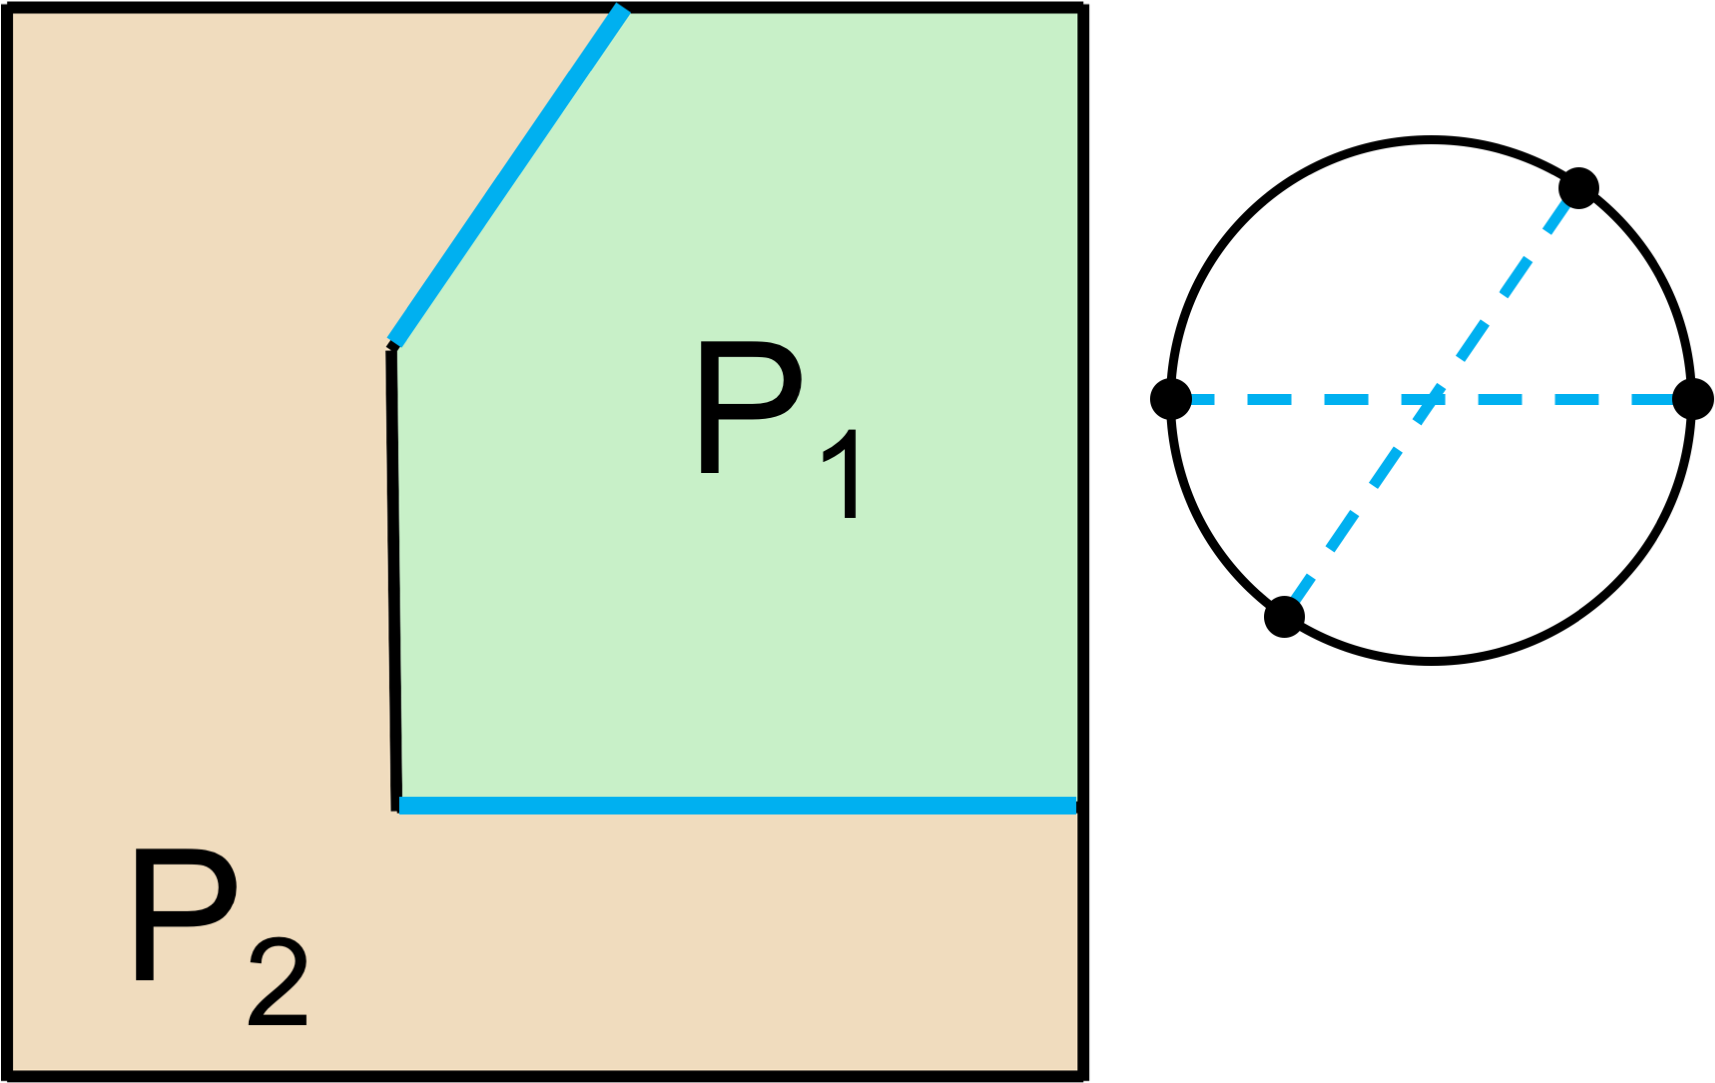
\includegraphics[width=0.32\columnwidth]{images/NDBG_Diameter.png}
	\vspace{-5pt}
\end{wrapfigure}
contact (e.g., $P_1$ and $P_2$ in the inset), if there are more than two contact lines, we only retain the two diameters of $C$ (e.g., two contact lines in blue) which bound the cone of directions in which one part is free to translate relative to the other.
The arrangement of points and intervals on $C$ and the associated DBGs form the {\em non-directional blocking graph} of $\mathbf{A}$; see Figure~\ref{fig:NDBG}(e).
% which represents the blocking relations among parts in $\mathbf{A}$ for all possible translation directions.
The NDBG for a 3D assembly can be built similarly by constructing DBGs for each regular region of a unit sphere that represents all possible translation direction in 3D; please refer to~\cite{Wilson-1994-GeometricReasoning} for more details.



\vspace*{1.0mm}
\noindent
{\bf Base Directional Blocking Graphs.} \
An NDBG represents the parts blocking relations with redundancy in two aspects.
First, the DBG corresponding to an arc in $C$ can be derived by performing union operations on the DBGs associated with the two end points of the arc; see again Figure~\ref{fig:NDBG}(e).
%This is because the blocking relations for $d = d_1$ and $d = d_2$ are the extreme case
%by performing union of the edges in these two graphs since \TODO{give a reason here}.
Second, we can obtain $G(-d, A)$ from $G(d, A)$ easily by reversing the direction of every edge in $G(d, A)$ due to the reciprocity of  blocking relations among the parts.

Therefore, it is sufficient to model the blocking relations in $\mathbf{A}$ by using only a set of {\em base DBGs} denoted as $\{G(d, A)\}$, which we select as the DBGs corresponding to the end points in a half circle of $C$.
For example, two DBGs in Figure~\ref{fig:NDBG}(c\&d) form $\{G(d, A)\}$.
We call the set of directions corresponding to the base DBGs as {\em base directions}, denoted as $\{d\}$.
%The number of base DBGs (as well as base directions) is $O(n^2)$ since every pair of parts provides either two (in contact) or zero (no contact) diameters in $C$.
The number of base DBGs (as well as base directions) is $O(n^2)$ since every pair of parts provides at most two diameters in $C$.  
%\Mark{Does this mean two contact parts cannot be blocked only along a single direction?}
%\Peng{You are right. Two contact parts are possible to provide one diameter. Text has been revised accordingly.}
%\Mark{better to have a figure showing 3D base DBGs}

%Hence, if a part of part group is movable along the direction within the arc, it must be movable also along the direction corresponding to one of the end points.
%Hence, when identifying movable parts or part groups,  we only need to test each direction corresponding to the end points (e.g., $-x, +x, -y, +y$ in Figure~\ref{fig:NDBG}).



%%%%%%%%%%%%%%%%%%%%%%%%%%%%%%%%%%%%%%%%%%%%%%%%
% Test Interlocking 
%%%%%%%%%%%%%%%%%%%%%%%%%%%%%%%%%%%%%%%%%%%%%%%%

\subsection{Testing Interlocking}
In an interlocking assembly, every part and every part group are immobilized for all possible translation directions, except a single key.
To test immobilization of a part group $\mathbf{S}$, we need to compute blocking relations between $\mathbf{S}$ and $\mathbf{A}-\mathbf{S}$:  the part group $\mathbf{S}$ is immobilized if $\mathbf{S}$ is blocked by $\mathbf{A}-\mathbf{S}$ in all translation directions.
Explicitly testing interlocking by checking immobilization of every part and every part group has exponential time complexity. 
However, treating each part group $\mathbf{S}$ independently ignores significant redundancies in the blocking relations across the parts.
%This huge complexity mainly arises from the redundancy of recomputing blocking relations for every parts group $\mathbf{S}$ by considering it as a totally new unit.
% rather than utilizing the computed blocking relations of $\mathbf{S}$'s component parts.
%
We exploit these redundancies and propose a more efficient approach to test global interlocking. 
The key idea is to utilize the blocking relations encoded in the set of base DBGs to implicitly test immobilization of every part and every part group along a finite number of translation directions, i.e., the base directions $\{d\}$.
In detail, an assembly with at least three parts is interlocking, if all base DGBs are either

\begin{enumerate}
\item strongly connected, or 
\item have only two strongly connected components one of which has a single part that is identical across all DGBs.
\end{enumerate}	
%\vspace*{-0.5mm}
Here the strongly connected component with a single part is the key of the assembly.
The direction $d$ associated with each DBG with two strongly connected components is the key part's (reversed) movable direction according to the in-edge (out-edge) of the key in the DBG.
For example, the assembly in Figure~\ref{fig:NDBG}(a) is interlocking and $P_1$ is the key since its two base DBGs in Figure~\ref{fig:NDBG}(c\&d) satisfy the above requirement.
% where $P_1$ is the key part and its movable direction is $\{d_2\}$.

In our implementation, we use Tarjan's algorithm~\cite{Tarjan-1972-SCC} to find the strongly connected components in each DBG. Runtime complexity is linear in the number of edges and nodes in the graph, i.e., $O(n^2)$ since there are at most $n^2$ edges in the graph.
As the set of base DBGs has $O(n^2)$ graphs, the worst-case complexity of our interlocking testing algorithm is $O(n^4)$, which is much lower than $O(2^n)$ of the previous approach~\cite{Song-2012-InterCubes}.
In particular, the complexity to test interlocking of a well-structured assembly, 
where each part connects with at most $L\ll n$ parts, is $O(L^2n^2)$ since the number of base DBGs is $O(Ln)$ and running Tarjan's algorithm on each DBG is also $O(Ln)$.
In practice, our algorithm is extremely fast. For example, our implementation can test for interlocking of the 80-piece \textsc{Bunny} assembly in Figure~\ref{fig:Result_Puzzle_Bunny}(b) in 1 millisecond, including the construction of all blocking graphs. For comparison, the approach of~\cite{Song-2012-InterCubes} takes 24.6 seconds on a 20-piece \textsc{Bunny} of the same voxel count and would run years on the 80-piece model.
See also Section~\ref{sec:results}.

%Our observation is that although the immobilization of a parts group $S$ cannot be derived from those of parts in the group, the blocking relations of the $S$ indeed can be derived.
 
%By using the based DBGs, we can consider an assembly as interlocking if all base DBGs are strongly connected, except a few ones where there is only a common node that does not have out-edges.
%Here, the common node is the key part while the directions associated with the non strongly connected DBGs are the key's movable directions.  



%%%%%%%%%%%%%%%%%%%%%%%%%%%%%%%%%%%%%%%%%%%%%%%%
% Test Disassemblability 
%%%%%%%%%%%%%%%%%%%%%%%%%%%%%%%%%%%%%%%%%%%%%%%%

\vspace*{1.0mm}
\noindent
{\bf Testing Disassemblability.} \
The DBGs were originally developed to test whether a structure can be (dis)assembled.
%The key observation is that a sub-graph (usually a strongly connected component) in a base DBG $G(d,A)$ with zero out-degree (in-degree) is movable along $d$ ($-d$).
%Hence, we can use the Algorithm~\ref{alg:DisasssTest} to find a sequence to disassemble parts in a 2D/3D assembly.
By successively identifying the movable part (or part group) based on the DBGs, we can find a sequence to disassemble all the parts. 
Otherwise, we consider the structure as not (dis)assemblable by translational part motions.

In practice, a part $P$ may not be able to be taken out by a single translation, say along $d$, since some part may block $P$ after it 
moves along $d$ for a certain distance; see the inset figure.
Since this case has 
\setlength{\columnsep}{13pt}
\begin{wrapfigure}{r}{0.30\columnwidth}
	\vspace{-12pt}
	\centering
	\hspace{-8pt}
	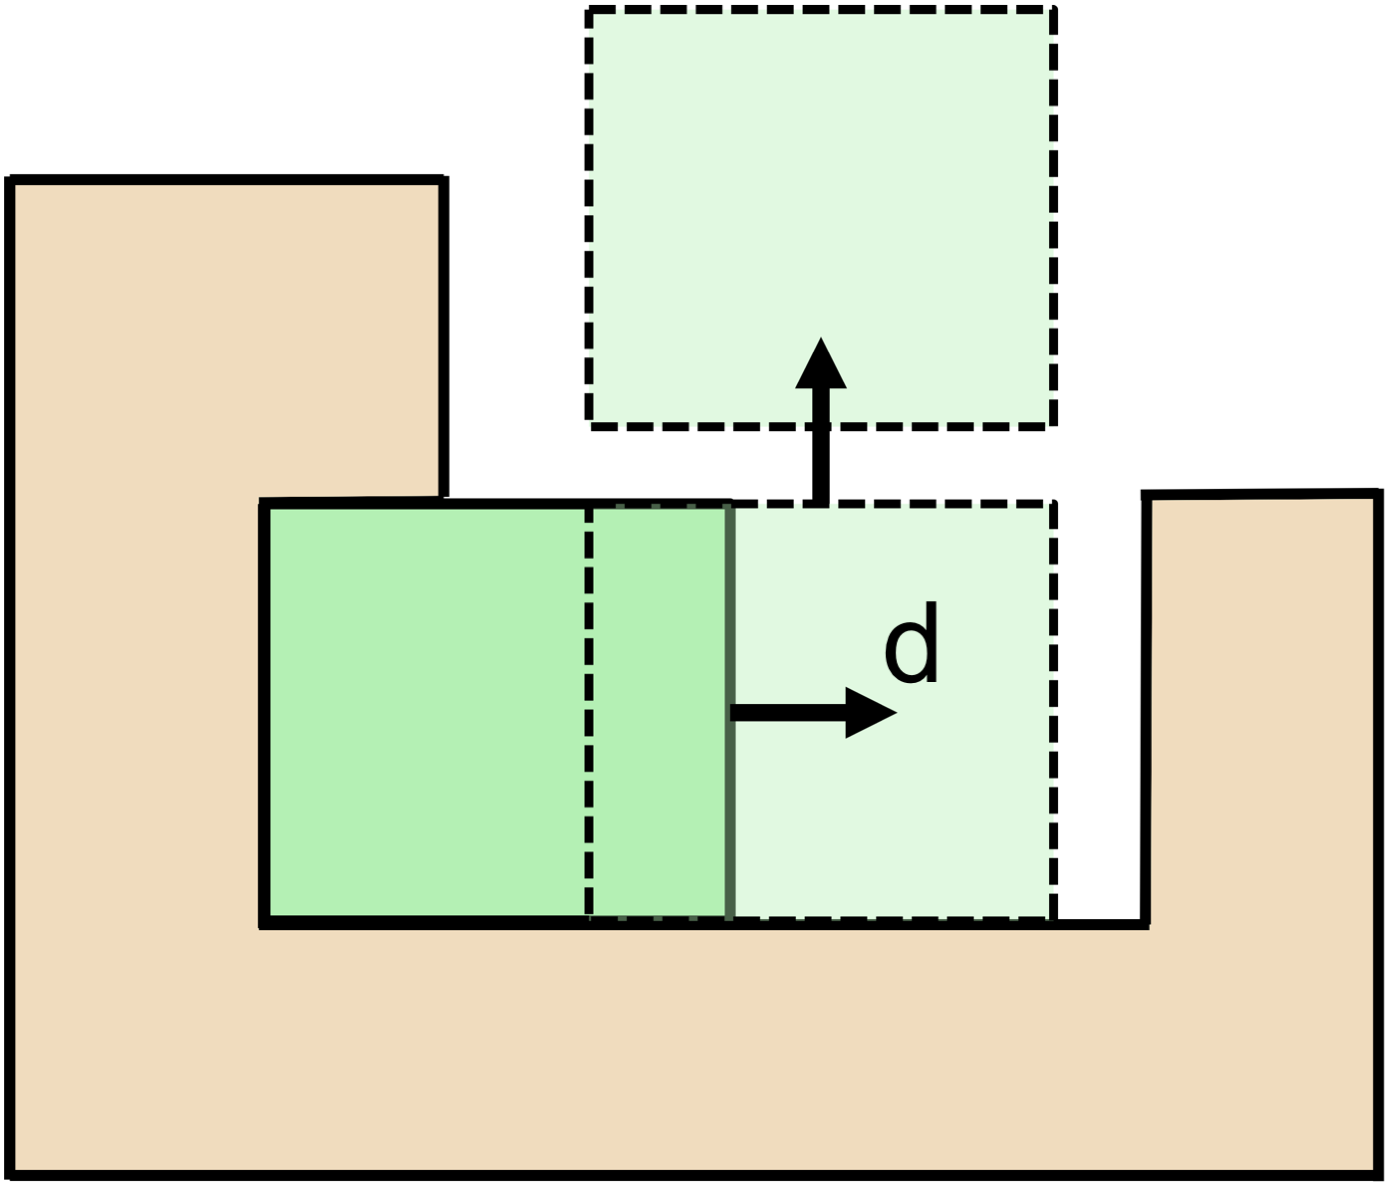
\includegraphics[width=0.28\columnwidth]{images/Multi_step.png}
	\vspace{-11pt}
\end{wrapfigure}
not been modeled in the DBGs, we use a sample-based approach to find a disassembly path of $P$ without parts collision.
%if $P$ cannot be directly taken out along $d$.
Alternatively, more complex disassembly path planning approaches, e.g.~\cite{Ghandi-2015-AssemblyPlanningReview}, could be employed here.










%%%%%%%%%%%%%%%%%%%%%%%%%%%%%%%%%%%%%%%%%%%%%%%%%%%%%%%%%%%%%%%%%%%%%%%%%%%%%%%%%%%%%%%%%%%%%%%%%%%
% Backup
%%%%%%%%%%%%%%%%%%%%%%%%%%%%%%%%%%%%%%%%%%%%%%%%%%%%%%%%%%%%%%%%%%%%%%%%%%%%%%%%%%%%%%%%%%%%%%%%%%%

\if 0
\vspace*{-2mm}
\begin{algorithm}
	\caption{TestDisassemblability($\mathbf{A}$)\ \vspace*{-2mm}}
	\label{alg:DisasssTest}
	\vspace*{1.0mm}
	\KwIn
	{
		\hspace{3.0mm}A 2D/3D assembly $\mathbf{A}$ \\
	}
	\vspace*{0.5mm}
	\KwOut
	{
		\hspace{0.1mm} Disassemblability of $\mathbf{A}$
	}
	\vspace*{2mm}
	Construct a set of base DBGs for $\mathbf{A}$ \;
	\While{ $\mathbf{A}$ is non-empty }
	{
		\vspace*{0.5mm}
		\If{Find a part $P$ whose out-degree (in-degree) is zero in one base DBG $G(d, A)$ }
		{
			Remove $P$ from $\mathbf{A}$ by tranlsating it along $d$ ($-d$) \;
			Update all base DBGs for the new $\mathbf{A}$ \;	
		}
		\ElseIf{Find a parts group $\mathbf{S}$ which is a stongly connected component  in one base DBG $G(d, A)$ and whose out-degree (in-degree) is zero in the DBG}
		{
			\If{TestDisassemblability($\mathbf{S})$ == true }
			{
				Remove parts in $\mathbf{S}$ together from $\mathbf{A}$ along $d$ ($-d$)  \;
				Update all base DBGs for the new $\mathbf{A}$ \;	
				Disassemble parts from $\mathbf{S}$ \;
			}
			\Else
			{
				Return false \;	
			}
		}
		\Else
		{
			Return false \;
		}
	}
	
	Return true \;
\end{algorithm}
\fi










%%%%%%%%%%%%%%%%%%%%%%%%%%%%%%%%%%%%%%%%%%%%%%%%%%%%%%%%%%%%%%%%%%%%%
% Overivew
%%%%%%%%%%%%%%%%%%%%%%%%%%%%%%%%%%%%%%%%%%%%%%%%%%%%%%%%%%%%%%%%%%%%

\begin{algorithm}[!t]
	\caption{Algorithm to design an interlocking assembly $\mathbf{A}_n$ from a given shape $R_0$.}
	\begin{algorithmic}[1]
		\Function{CreateInterlockAssembly}{$R_0$}

		\State $i \gets 0$
		\State $A_i^{*} \gets [R_0]$
				
		\While {$i < n$} 
		\If{ $i$=0}
		\State{$\{A_{i+1} \}$  $\gets$ GenerateKey($A_i^{*}$)	}  \Comment{See Subsection~\ref{subsec:genKey}}
		\If{$\{A_{i+1} \} = \emptyset$}
		\State   \Return NULL 
		\EndIf
		
		\Else
		\State $\{A_{i+1} \}$ $\gets$ GenerateParts($A_i^{*}$)  \Comment{See Subsection~\ref{subsec:genPart}}
		\EndIf
		
		\vspace{1.0mm}
		\If{$\{A_{i+1} \} \neq \emptyset$}
		\State RankCandidates($\{A_{i+1} \}$)     \Comment{In descending order}   % { i.e., $A_{i+1}^1$ is the best one }
		\If{ $i+1 =  n$}
		\State   \Return $A_n^1$				
		\Else
		\State 	$i \gets i+1$  
		\State $A_i^{*} \gets A_{i}^1$ 
		\EndIf
		
		\ElsIf{$A_i^{*}.sibling \neq NULL$}  
		\State	$A_i^{*} \gets A_i^{*}.sibling$   \Comment{$A_i^{*}.sibling$ is the one second to $A_i^{*}$ in the ranked $\{A_{i} \}$}
		
		\Else
		\While{$A_i^{*}.parent \neq$ NULL $\&\&$  \\  \hspace{22.0mm}   $A_i^{*}.parent.sibling =$ NULL}
		\State	$A_i^* \gets A_i^{*}.parent$ 
		\State $i \gets i-1$
		\If {$i= 0$}   \Comment{Quit if backtrack to $A_0$  }
		\State{\Return NULL}
		\EndIf
		\EndWhile
		
		\If {$A_i^{*}.parent \neq$ NULL $\&\&$ \\ \hspace{17.0mm} $A_i^{*}.parent.sibling  \neq$ NULL}
		\State $A_i^* \gets A^*.parent.sibling$			
		\Else      
		\State	\Return NULL 
		\EndIf
		
		\EndIf
		
		\EndWhile
		
		\EndFunction
	\end{algorithmic}
	\label{alg:Alg_Framework}
\end{algorithm}

\section{Computational Design Framework}
\label{sec:approach}

%%%%%%%%%%%%%%%%%%%%%%%%%%%%%%%%%%%%%%%%%%%%%%%%
% Problem Formulation
%%%%%%%%%%%%%%%%%%%%%%%%%%%%%%%%%%%%%%%%%%%%%%%%

%\Mark{I think this section needs an overview first. Below we describe an iterative procedure that could fail at several locations. But we do not describe what happens in such a case. Do we back-track? Start over? How do we avoid making bad decisions early on whose consequences will only become apparent much later?
%What can we say about the outcome of the method. If it doesn't find a solution, can we guarantee that none exits? Or in other words, if a solution exists, are we guaranteed to find it? We should probably explain upfront the two-stage approach and motivate why it makes sense, but also mention what the drawbacks are.}

%\vspace*{1.0mm}
%\noindent
%{\bf Problem Formulation.}  \
Given our efficient algorithm to test for interlocking, our main goal is now to provide effective algorithms for designing interlocking assemblies. We first provide a high-level overview of our framework before presenting the conceptual and algorithmic details.

As input we expect the final shape of the assembly, from which the component parts are either constructed from scratch as in~\cite{Xin-2011-BurrPuzzles, Song-2012-InterCubes,Song-2015-Interlock} or explicitly initialized as in~\cite{Fu-2015-Furniture, Song-2016-CoFiFab,Yao-2017-InterlockShell}.
%Requirements on the geometry of the parts (e.g., for fabrication) and/or the final assembly (e.g., aesthetics) may need to be considered in the design process, depending on the application.
%
%For the latter case, the neighboring relationship among the parts have been given, which define the set of part pairs for constructing blocking relations. 
Our computational process for creating an interlocking assembly starts with the full input model, then iteratively splits off successive parts for disassembly. At each iteration, we first identify a set of suitable blocking relations between the current assembly and the new part to be generated such that the interlocking property is maintained. Then we search for the part geometry that satisfies these blocking relations. The selection of a new part is guided by a ranking function that takes into account certain geometric properties, e.g. part size, or other requirements, e.g. on part fabrication.
The search space is then explored in a tree traversal process that uses automatic backtracking when no interlocking solution could be found in a specific iteration. We also provide a user interface to interactively explore different options for part decomposition, allowing the user to  overwrite the generic ranking function for part selection.



%%%%%%%%%%%%%%%%%%%%%%%%%%%%%%%%%%%%%%%%%%%%%%%%
% Iterative Design Framework
%%%%%%%%%%%%%%%%%%%%%%%%%%%%%%%%%%%%%%%%%%%%%%%%

\subsection{Iterative Design Framework}
\label{subsec:framework}

%\vspace*{1.0mm}
%\noindent
%{\bf Iterative Design Framework.}  \
Given the input shape denoted as $R_0$, we iteratively construct the geometry of each part (or introduce appropriate joints in the geometry of each initialized part; see Section~\ref{subsec:furniture}), one by one. This forms a sequence of constructed parts, $P_1$, $P_2$, $...$, $P_n$, with $R_n$, the remaining part of $R_0$, as the last part:
%In other words, we iteratively partition remaining part $R_{i-1}$ into two parts to form $P_i$ and $R_i$:
\begin{displaymath}
[R_0] \rightarrow [P_1,R_1] \rightarrow [P_1,P_2,R_2] \rightarrow ... \rightarrow [P_1,...P_n,R_n] \ .
\end{displaymath}
Here we denote each intermediate assembly $[P_1, ..., P_i, R_i]$ as $\mathbf{A}_{i}$ ($0 \leq i \leq n$), and its base DBGs as $\{ G(d, A_i) \}$. 
Figure~\ref{fig:Framework_Overview} shows an example where the parts are constructed from scratch.


%When parts have been initialized, we consider all those untouched parts as $R_{i-1}$ ($i\geq1$) conceptually when constructing $P_i$ and $R_i$ from it. 
%\Peng{Would it be sufficient to guarantee interlocking by constructing a single piece at a time; e.g., shall we construct a few pieces together for furniture?}

% Requirements on the construction of $P_i$ and $R_i$
To guarantee that the resulting assembly $\mathbf{A}_n = [P_1, ..., P_n, R_n]$ is interlocking and disassemblable, we have the following requirements when decomposing $R_{i-1}$ into $P_i$ and $R_i$:
\begin{enumerate}[label=(\roman*), leftmargin=*]
	\vspace*{-0.5mm}
	\item
	{\em  Connected.} \
   The geometries of $P_i$ and $R_i$ should each be simply connected, making $\mathbf{A}_i$ a valid assembly. 
   
   	\vspace*{0.5mm}
    \item
   {\em Interlocking.} \
   $\mathbf{A}_i$ ($i\geq2$) is interlocking with $P_1$ as the key.
   In other words, $\{G(d, A_i)\}$ should satisfy the interlocking requirement described in Section~\ref{sec:model}.
   %This is achieved by constructing the geometry of $P_i$ and $R_i$ to satisfy the two interlocking requirements on $\{G(d, A_i)\}$. 

   	\vspace*{0.5mm}
   	\item
   	{\em Disassemblable.} \
   	$P_i$ can be removed from $[P_i, R_i]$, so we can disassemble $\mathbf{A}_i$ in the order of construction $P_1$, $P_2$,  $...$,  $P_i$, $R_i$.
   	
	%try to find the fewest internal blocking relations to be constructed between $P_i$ and $R_i$ such that the strongly connected property is preserved; see Figure~\ref{fig:Framework_Conceptual}(d).
	%This is because fewer internal blocking relations provide more flexibility to construct the geometry of $P_i$ and $R_i$.	
\end{enumerate}	
\vspace*{-0.5mm}
\noindent
The advantage of this iterative design framework is that we achieve the goal of global interlocking by satisfying a set of local requirements when constructing each pair of $P_i$ and $R_i$.

\vspace*{1.0mm}
\noindent
{\bf Tree Traversal.}  \
Since we cannot guarantee that the construction of $P_i$ and $R_i$ succeeds at every iteration, we propose an iterative approach with backtracking to construct $\mathbf{A}_n$; see Figure~\ref{fig:Framework_Overview} and Algorithm~\ref{alg:Alg_Framework}.
The key idea is to build and maintain a construction tree, where each node represents a candidate of $\mathbf{A}_i$. For each node we generate a set of children denoted as $\{\mathbf{A}_{i+1}\}$. 
% by generating a set of $\mathbf{A}_{i+1}$ denoted as $\{\mathbf{A}_{i+1}\}$ from $\mathbf{A}_{i}$ at each iteration.
% by trying different ways of partitioning $R_{i-1}$ into $P_i$ and $R_i$.
Our approach ranks these candidate assemblies at each iteration to facilitate the construction of successive parts.
For example, we rank $\{\mathbf{A}_{i+1}\}$ according to the compactness of $R_{i+1}$, since parts extracted from a compact $R_{i+1}$ are more likely to be simply connected; compare $R_1$ in Figure~\ref{fig:Framework_Overview}(c\&f). 
In case the user has other design goals besides interlocking, e.g., regarding the appearance of the assembly, we support user intervention to adjust the ranking.
%
In case we cannot generate any valid result from the selected candidate in $\{\mathbf{A}_{i+1}\}$, we can backtrack the tree to try other nodes without restarting the whole design process.
The size of $\{\mathbf{A}_{i+1}\}$ is denoted as $M$.
A large $M$ requires more time for generating $\{\mathbf{A}_{i+1}\}$, but also provides more choices for ranking and backtracking. We set $M = 30$ by default in our experiments but it can be adjusted, depending on the input model. 

%In case users have other requirements on the assembly besides interlocking (e.g., appearance), our framework supports user intervention to adjust the ranking.}
%\Mark{We should have a forward reference to an example of user intervention. In general, right now it remains abstract what exactly the ranking function is.}
%\Peng{Text has been revised accordingly.}

%Our framework cannot guarantee to find a solution if it exists, nor guarantee non exists if we cannot find any solution.
%These questions can be answered by exhaustive search only in very small scale design problems; see the experiment in Section~\ref{sec:results}.
%The usefulness of our framework is to provide general computational support for users to design interlocking assemblies according to their desires, which is extremely challenging for manual effort.
Below we explain our approach to generate the key part (Subsection~\ref{subsec:genKey}) and the remaining parts of the assembly (Subsection~\ref{subsec:genPart}). These steps can be customized to design different kinds of interlocking assemblies as discussed in Section~\ref{sec:results}.
Here, we take 2D interlocking puzzle design as an example for illustration.



%Thanks to the DBG-based representation, we can test and further guarantee interlocking for each intermediate assembly $\mathbf{A}_i$ efficiently. %which is previous works~\cite{Song-2012-InterCubes,Fu-2015-Furniture} intentionally skip this step due to the exponential complexity of their interlocking testing algorithm.



%which is achieved by performing the DBG-based interlocking test described in Section~\ref{sec:model}. 
%Note that this interlocking test is intentionally skipped by previous works~\cite{Song-2012-InterCubes,Fu-2015-Furniture} due to their exponential complexity of brute-force search.
%Lastly, we ensure that $A_i$ is disassemblable by requiring $P_j$ to be separable from $R_j$ for every pair of $[P_j, R_j]$, where $1 \leq j \leq i$.
%By this, we guarantee that the resulted assembly $A_n = [P_1, ..., P_n, R_n]$ is interlocking and disassemblable.


\begin{figure*}[!t]
	\centering
	%\vspace*{-3.5mm}
	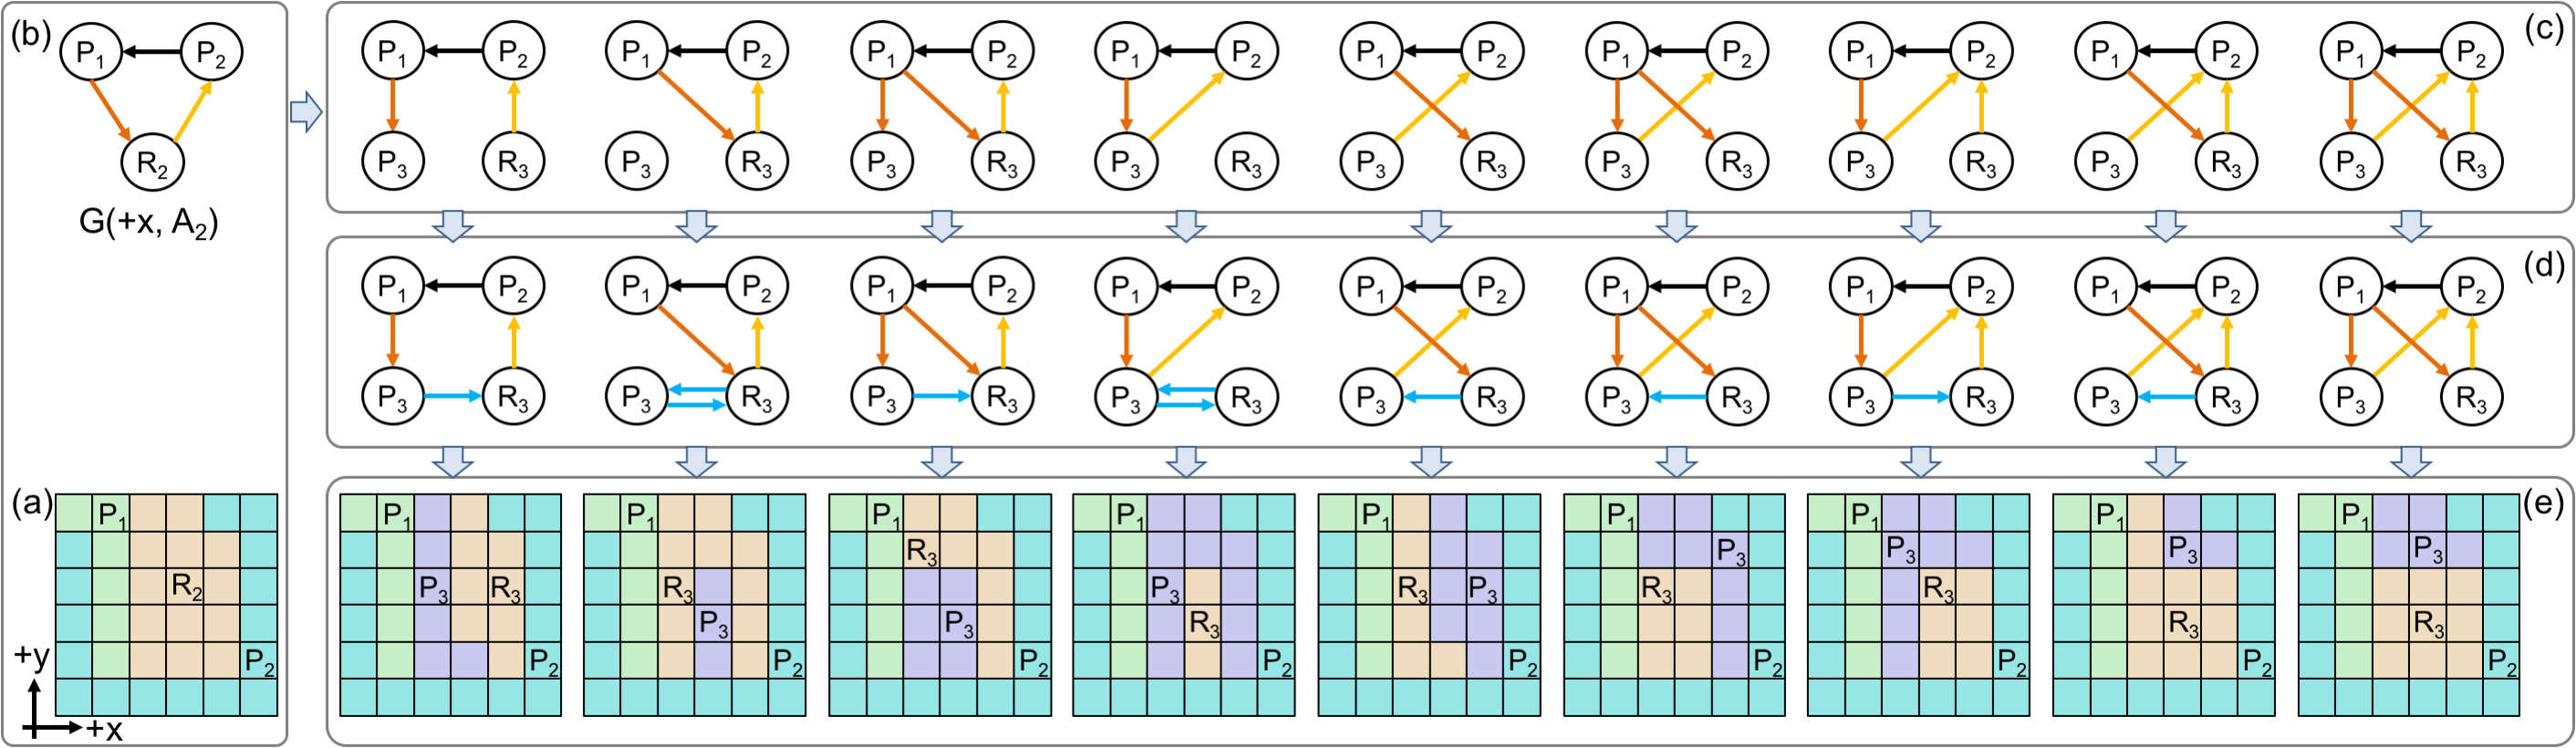
\includegraphics[width=17.80cm]{images/Framework_Conceptual.png}
	\vspace*{-2.5mm}
	\caption{
		(a) An intermediate assembly $\mathbf{A}_2$ and 
		(b) its base DBG $G(+x, A_2)$, where the in-edge and out-edge of $R_2$ are colored in dark and light orange respectively;
		(c) all cases of distributing existing blocking relations (dark and light orange edges) to $P_3$ and $R_3$; 
		(d) the interlocking graph designs that require the fewest internal blocking relations (blue edges) between $P_3$ and $R_3$; and
		(e) the corresponding geometric examples.
	}
	\vspace*{-1.0mm}
	\label{fig:Framework_Conceptual}
\end{figure*}

\begin{figure*}[!t]
	\centering
	%\vspace*{-3.5mm}
	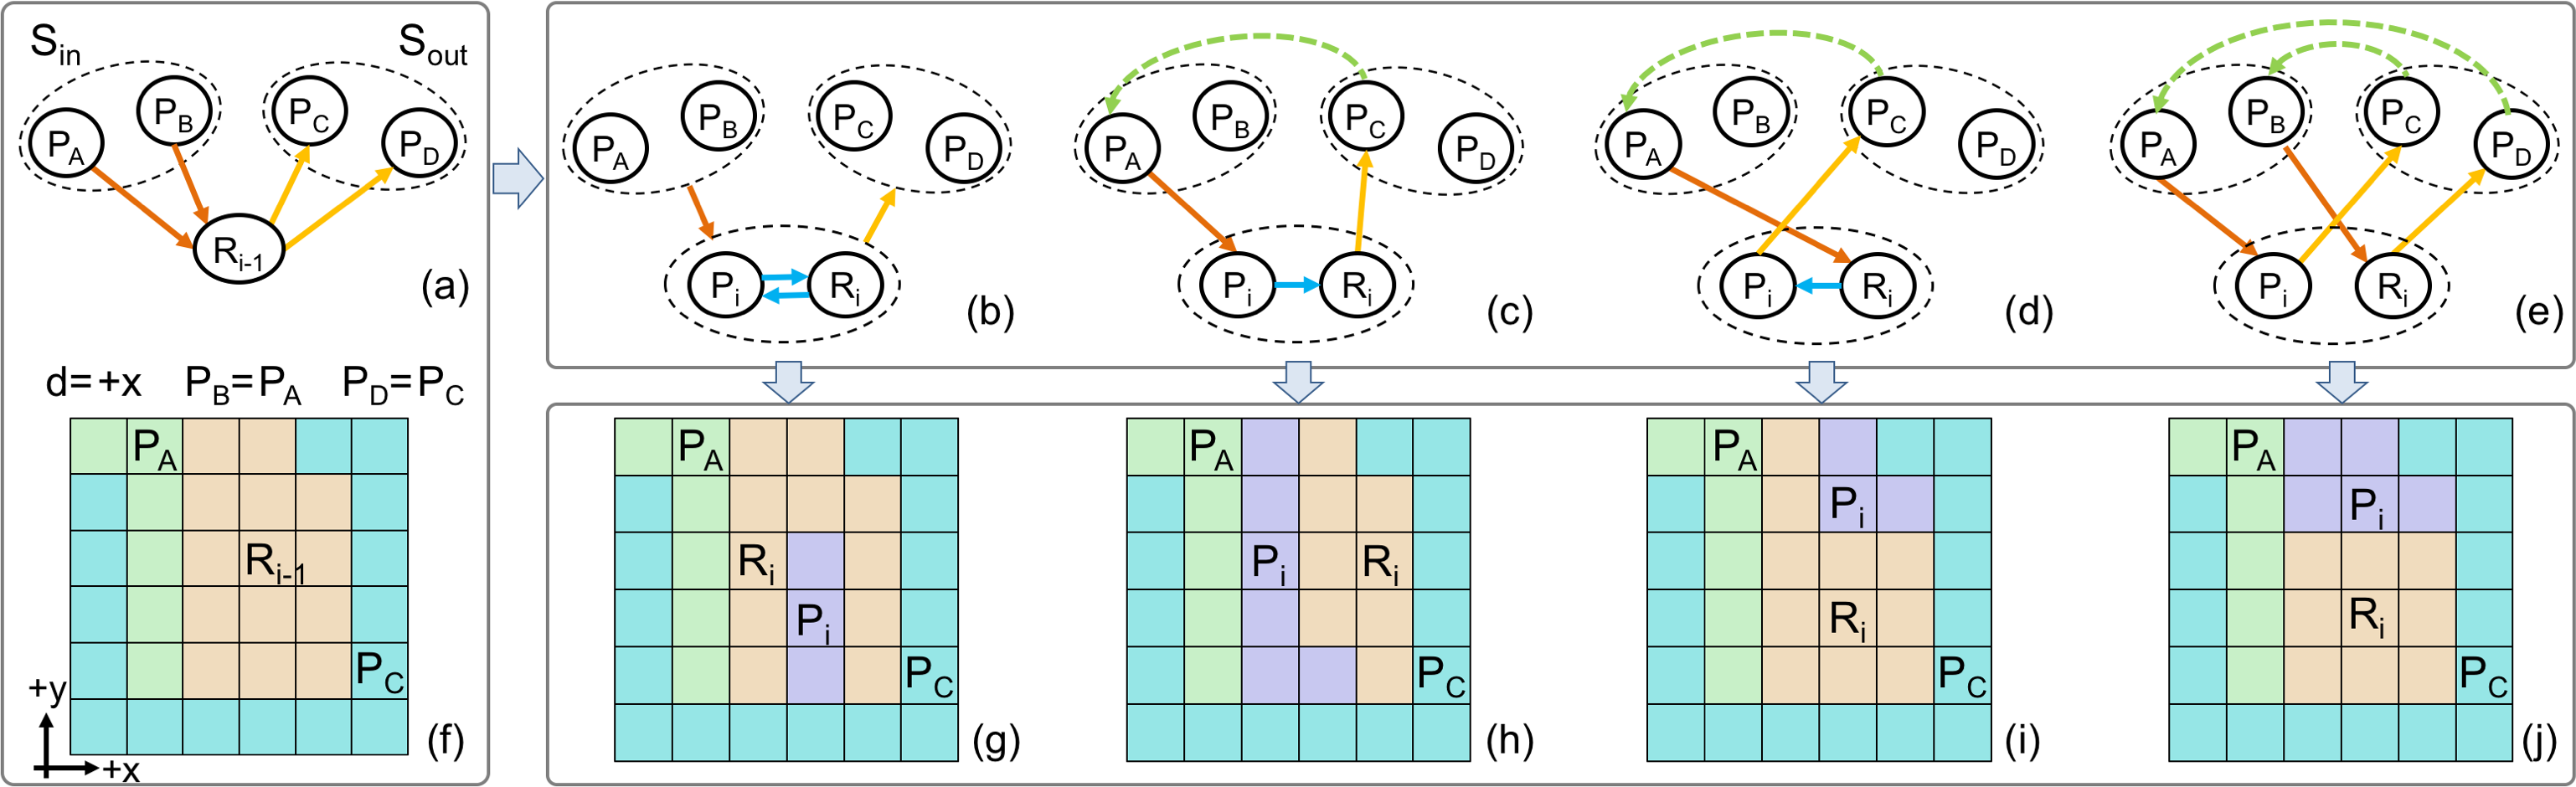
\includegraphics[width=14.50cm]{images/Framework_Cycle.png}
	\vspace*{-2.5mm}
	\caption{
		(a) Given $G(d, A_{i-1})$, (b-e) we ensure that $G(d, A_i)$ is strongly connected by constructing a cycle that includes both $P_i$ and $R_i$.
		A dashed ellipse in (a-e) indicates a subset of parts, i.e., $S_{in}$, $S_{out}$, and $\{P_i, R_i\}$, where $S_{in}$ ($S_{out}$) denotes the set of parts with an edge to (from) $R_{i-1}$.
		The directed edges from (to) a dashed circle in (b) indicate that the edge can be from (to) any part in the associated subset.
		The dashed green edges in (c-e) indicate that a part can reach the other part in $G(d, A_{i-1})$ without passing through $R_{i-1}$.
		(f-i) Geometric examples corresponding to (a-e), where $d = +x$, $S_{in} = \{P_A\}$, and $S_{out} = \{P_C\}$.
		%\Mark{I find this figure confusing. We have $P_A$, etc. in the top row, but below we show something different, i.e. $P_1$. Can't we find an example that is consistent? We should probably also specify $d$.}
		%\Peng{The symbols have been revised in the figure. I have spent an hour in trying to design a more complex 2D example with 6 pieces but failed. Such a example that shows all four cases together seems not easy to find.}
	}
	\vspace*{-2.5mm}
	\label{fig:Framework_Cycle}
\end{figure*}



%%%%%%%%%%%%%%%%%%%%%%%%%%%%%%%%%%%%%%%%%%%%%%%%
% Generate P_1 and R_1
%%%%%%%%%%%%%%%%%%%%%%%%%%%%%%%%%%%%%%%%%%%%%%%%

\vspace*{-0.8mm}
\subsection{Generating the key}
\label{subsec:genKey}

We first partition the input model $R_0$ into $P_1$ and $R_1$, where $P_1$ is the key and $R_1$ is the remaining part.
We construct the geometry of $P_1$ following the procedure in~\cite{Song-2012-InterCubes}; i.e., select a seed pixel, ensure its blocking and mobility, and expand the key piece.
Recall that the key is the only movable (thus unstable) part in an interlocking assembly.
Therefore, we restrict $P_1$ to have a single movable direction in $\mathbf{A}_1$ denoted as $d_1$, and usually select $d_1$ being upward to stabilize $P_1$ with gravity; see Figure~\ref{fig:Framework_Overview}(b\&c) for two examples.
We rank the candidates in $\{\mathbf{A}_1\}$ according to the compactness of $R_1$.
% since more compact $R_1$ will encourage generation of successive parts. 


%%%%%%%%%%%%%%%%%%%%%%%%%%%%%%%%%%%%%%%%%%%%%%%%
% Generate P_i and R_i
%%%%%%%%%%%%%%%%%%%%%%%%%%%%%%%%%%%%%%%%%%%%%%%%

\vspace*{-0.8mm}
\subsection{Generating $P_i$ and $R_i$ $(i>1)$} 
\label{subsec:genPart}
Next, we construct $P_i$ and $R_i$ from $R_{i-1}$ in two stages: {\em graph design} and {\em geometry realization}.
The first stage constructs base DBGs $\{G(d, A_i)\}$ that satisfy the interlocking requirement conceptually while the second stage aims at realizing the blocking relations described in $\{G(d, A_i)\}$ in the embedded geometry.
Note that geometric constraints (e.g., supported joint types) can be used to simplify graph design by eliminating  potential graph edges that cannot be realized geometrically anyway.


%%%%%%%%%%%%%%%%%%%%%%%%%%%
% Conceptual Design of P_i and R_i
%%%%%%%%%%%%%%%%%%%%%%%%%%%

\vspace*{1.0mm}
\noindent
{\bf Graph Design for $P_i$ and $R_i$.}  \
Starting from $\mathbf{A}_{i-1}$ ($i \geq 2$),  the goal is to find blocking relations for $P_i$ and $R_i$  such that the updated assembly $\mathbf{A}_{i}$ is still interlocking.
In other words, after splitting $R_{i-1}$ into $P_i$ and $R_i$ in $\{G(d, A_{i-1})\}$ to form $\{G(d, A_i)\}$, we need to construct a set of new edges of $P_i$ and $R_i$ in each $G(d, A_i)$ such that the graph remains strongly connected, except the key; see Figure~\ref{fig:Framework_Overview}.
To achieve this goal, we first classify blocking relations to be constructed into two classes:
\begin{enumerate}[label=(\roman*), leftmargin=*]
	\vspace*{-0.5mm}
	\item
	{\em External blocking relations} between $\{P_1, ..., P_{i-1}\}$ and $P_i$, as well as those between $\{P_1, ..., P_{i-1}\}$ and $R_i$ are inherited from those between  $\{P_1, ..., P_{i-1}\}$ and $R_{i-1}$.
	Thus, we need to distribute these existing blocking relations to $P_i$ and $R_i$; see Figure~\ref{fig:Framework_Conceptual}(c).
	
	\vspace*{0.5mm}
	\item
	{\em Internal blocking relations} between $P_i$ and $R_i$.
	For each case of distribution of external blocking relations, we may need to construct internal blocking relations between $P_i$ and $R_i$ such that each $G(d, A_i)$ remains strongly connected\footnote
	{If the key is movable along $d$, $G(d, A_i)$ is strongly connected without considering the key. Otherwise, the whole graph of $G(d, A_i)$ is strongly connected.}; see Figure~\ref{fig:Framework_Conceptual}(d).
	
	%try to find the fewest internal blocking relations to be constructed between $P_i$ and $R_i$ such that the strongly connected property is preserved; see Figure~\ref{fig:Framework_Conceptual}(d).
	%This is because fewer internal blocking relations provide more flexibility to construct the geometry of $P_i$ and $R_i$.	
\end{enumerate}	


\begin{figure*}[!t]
	\centering
	%\vspace*{-3.5mm}
	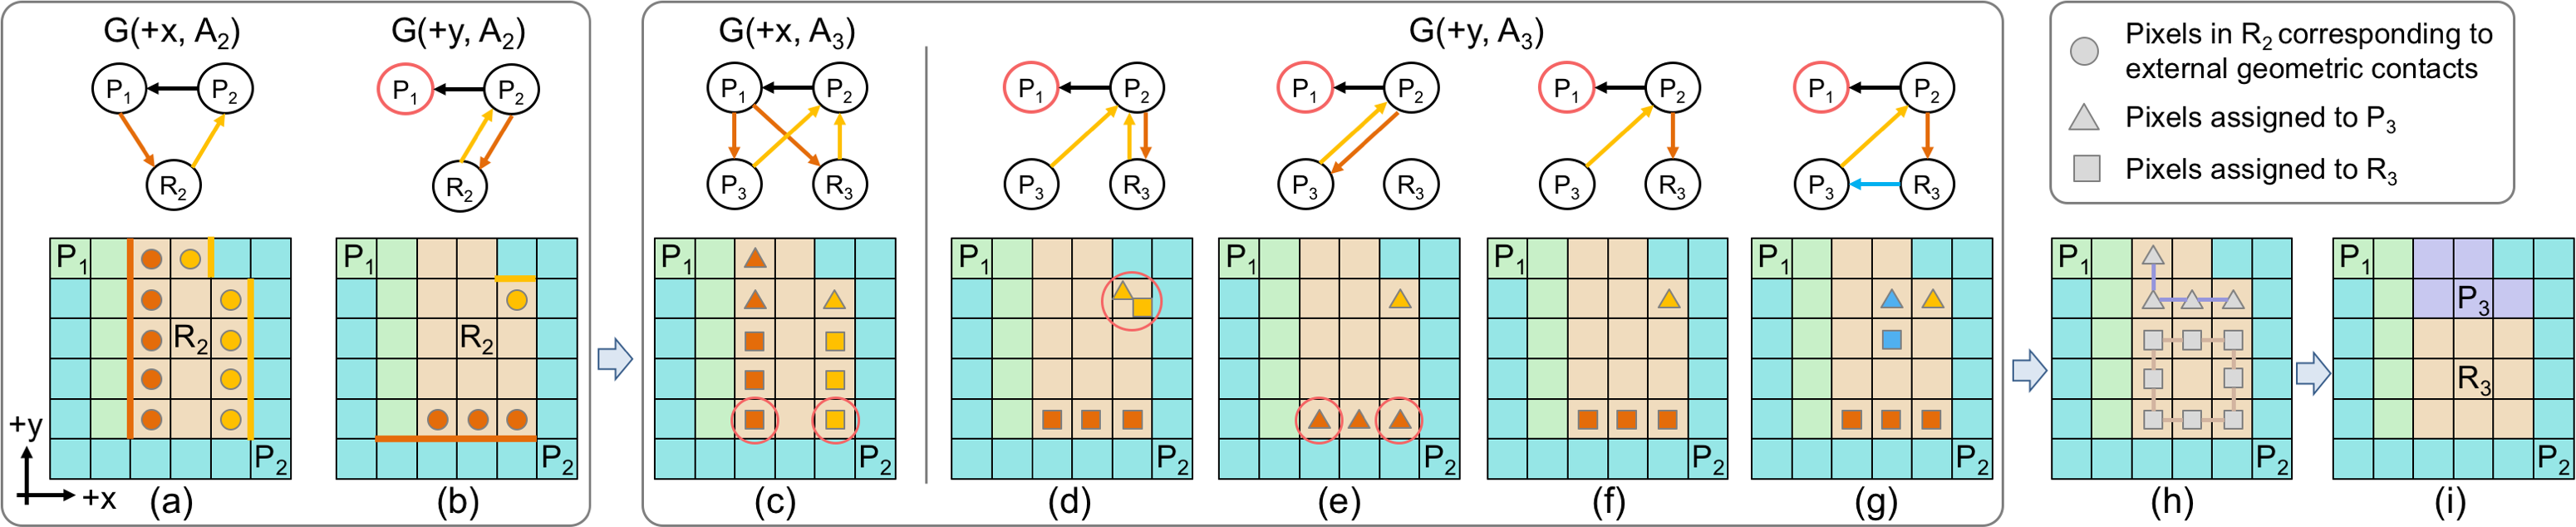
\includegraphics[width=17.80cm]{images/Framework_Geometry.png}
	\vspace*{-2.5mm}
	\caption{
		Geometry realization of $\{G(d, A_3)\}$.
		(a\&b) Identify geometric contacts between $\{P_1, P_2\}$ and $R_2$ in $\mathbf{A}_2$.
		(c-f) Distribute external geometric contacts between $P_3$ (shows as triangles) and $R_3$ (shown as squares) for (c) $G(+x, A_3)$ and (d-f) $G(+y, A_3)$,
		where (d\&e) show two failure examples.
		(g) Realize internal blocking relation between $P_3$ and $R_3$ in $G(+y, A_3)$.
		(h) Construct initial geometry of $P_3$ and $R_3$.
		(i) Resulting $\mathbf{A}_3$.
	}
	\vspace*{-2.0mm}
	\label{fig:Framework_Geometry}
\end{figure*}

\vspace*{-1.0mm}
Given these observations, we could find all valid graph designs by enumerating the distribution of external blocking relations, constructing the corresponding internal blocking relations, and testing the strongly connected property of the DBGs.
However, this generate-and-test approach could be very inefficient. The number of choices to distribute external blocking relations is $3^L$, where $L$ is the number of  edges of $R_{i-1}$ in $G(d, A_{i-1})$, since each edge of $R_{i-1}$ can be distributed to $P_i$, $R_i$, or both.
Figure~\ref{fig:Framework_Conceptual} shows an example with $3^2 =9$ graph designs, where $L=2$.



Rather than enumerating all possible graph designs, we propose an efficient approach to find a desired number of designs that are interlocking conceptually; see Figure~\ref{fig:Framework_Cycle}.
%\Mark{We need to be careful here. This statement suggest we look only at some subset of valid designs. Which subset is this? Are we not exploring the full search space?}
%\Peng{We are exploring the full search space since we can create blocking relation between $P_i$ and any other part (i.e., $\{P_1, ..., P_{i-1}\}$ and $R_i$) to immobilize $P_i$. The reason to find a few valid conceptual designs is due to the huge search space. 
%If we try to enumerate all of them, it is going to be a problem with exponential complexity. }
The key idea is to directly guarantee that each $G(d, A_i)$ is strongly connected by constructing a cycle in the graph that includes both $P_i$ and $R_i$, given that $G(d, A_{i-1})$ is already strongly connected.
%Denote the set of parts with an edge to (from) $R_{i-1}$ as $S_{in}$ ($S_{out}$).
Denote $S_{in}$ ($S_{out}$) as the set of parts with an edge to (from) $R_{i-1}$, and $P_{in}$ ($P_{out}$) as an arbitrary part in $S_{in}$ ($S_{out}$); see Figure~\ref{fig:Framework_Cycle}(a\&f).
According to the number of internal blocking relations to be constructed between $P_i$ and $R_i$ denoted as $K$,  we have the following three cases to construct the cycle that we can choose independently for each DBG. 
%\Mark{To the reader it might not be clear if these cases occur, or if we can arbitrarily choose any of the three.}
%\Peng{The motivation is to control the degree of connection strength by interlocking, depending on the users intent.
%We can either make an interlocking assembly with fewest number of blocking relations (case 3; easy to be realized but may not be steady) or with lots of redundant blocking relations (case 1 and 2; hard to be realized but more steady even during the intermediate assembly state). }

%analyze the edges of $R_{i-1}$ and search external blocking relations based on internal blocking relations between $P_i$ and $R_i$ to ensure that the base DBG is strongly connected.

\begin{enumerate}[label=(\arabic*), leftmargin=*]
	\vspace*{-0.5mm}
	\item
	{\em K=2.}  \
	$P_i \rightarrow  R_i \rightarrow  P_i$ forms a cycle, i.e., any distribution of external blocking relations works for this case; see Figure~\ref{fig:Framework_Cycle}(b).

	\vspace*{0.5mm}
	\item
	{\em K=1.} \
	$P_i \rightarrow  R_i \rightarrow  P_{out} \dashrightarrow P_{in} \rightarrow P_i$ ($R_i \rightarrow  P_i \rightarrow  P_{out} \dashrightarrow P_{in} \rightarrow R_i$) forms a cycle if the single directed edge is from $P_i$ to $R_i$ (from $R_i$ to $P_i$); see Figure~\ref{fig:Framework_Cycle}(c\&d).
    Here, $P_{out} \dashrightarrow P_{in}$ means that $P_{out}$ can reach $P_{in}$ in $G(d, A_{i-1})$ without passing through $R_{i-1}$, or $P_{out}$ and $P_{in}$ are the same part.

	\vspace*{0.5mm}
	\item
	{\em K=0.} \
	$P_i \rightarrow  P_{out} \dashrightarrow  P_{in} \rightarrow R_i \rightarrow  P_{out}^{'} \dashrightarrow P_{in}^{'} \rightarrow P_i$ forms a cycle, where $P_{in}$ and $P_{in}^{'}$ (as well as $P_{out}$ and $P_{out}^{'}$) are possible to be the same part; see Figure~\ref{fig:Framework_Cycle}(e).
	%In this case, no internal blocking relation needs to constructed since external blocking relations are sufficient to make the graph strongly connected; see Figure~\ref{fig:Framework_Conceptual}(d) rightmost for an example.
	
	%This is because fewer internal blocking relations provide more flexibility to construct the geometry of $P_i$ and $R_i$.	
\end{enumerate}	

Compared with case 1, cases 2 and 3 rely more on external blocking relations than on internal blocking relations to immobilize $P_i$ and $R_i$.
As a consequence, these two cases impose fewer constraints on the subsequent geometry construction of $P_i$ and $R_i$,  resulting in a higher chance to be successfully realized in the embedded geometry; compare the geometric examples in Figure~\ref{fig:Framework_Cycle}(g-j).

Besides interlocking, we also need to ensure that $P_i$ is disassemblable in $[P_i, R_i]$.
Thus, we require that $P_i$ and $R_i$ have fewer than two directed edges (i.e., case 2 and 3) in at least one base DBG.
The output of this stage is a set of $\{G(d, A_i)\}$ that satisfy the interlocking requirement, denoted as $\mathbf{C}_i$.

\if 0
Among all the generated conceptual designs, we prefer to select those that rely on more external blocking relations than internal blocking relations (i.e., above case 2 and 3) since these designs have fewer constraints on geometry construction of $P_i$ and $R_i$, resulting a higher chance to be successfully realized in the embedded geometry.
\fi





%\Peng{there are too many choices for the conceptual designs; how do we select good ones from them?}


%%%%%%%%%%%%%%%%%%%%%%%%%%%
% Geometry Realization of P_i and R_i
%%%%%%%%%%%%%%%%%%%%%%%%%%%

\begin{figure}[!b]
	\centering
	\vspace*{-3.5mm}
	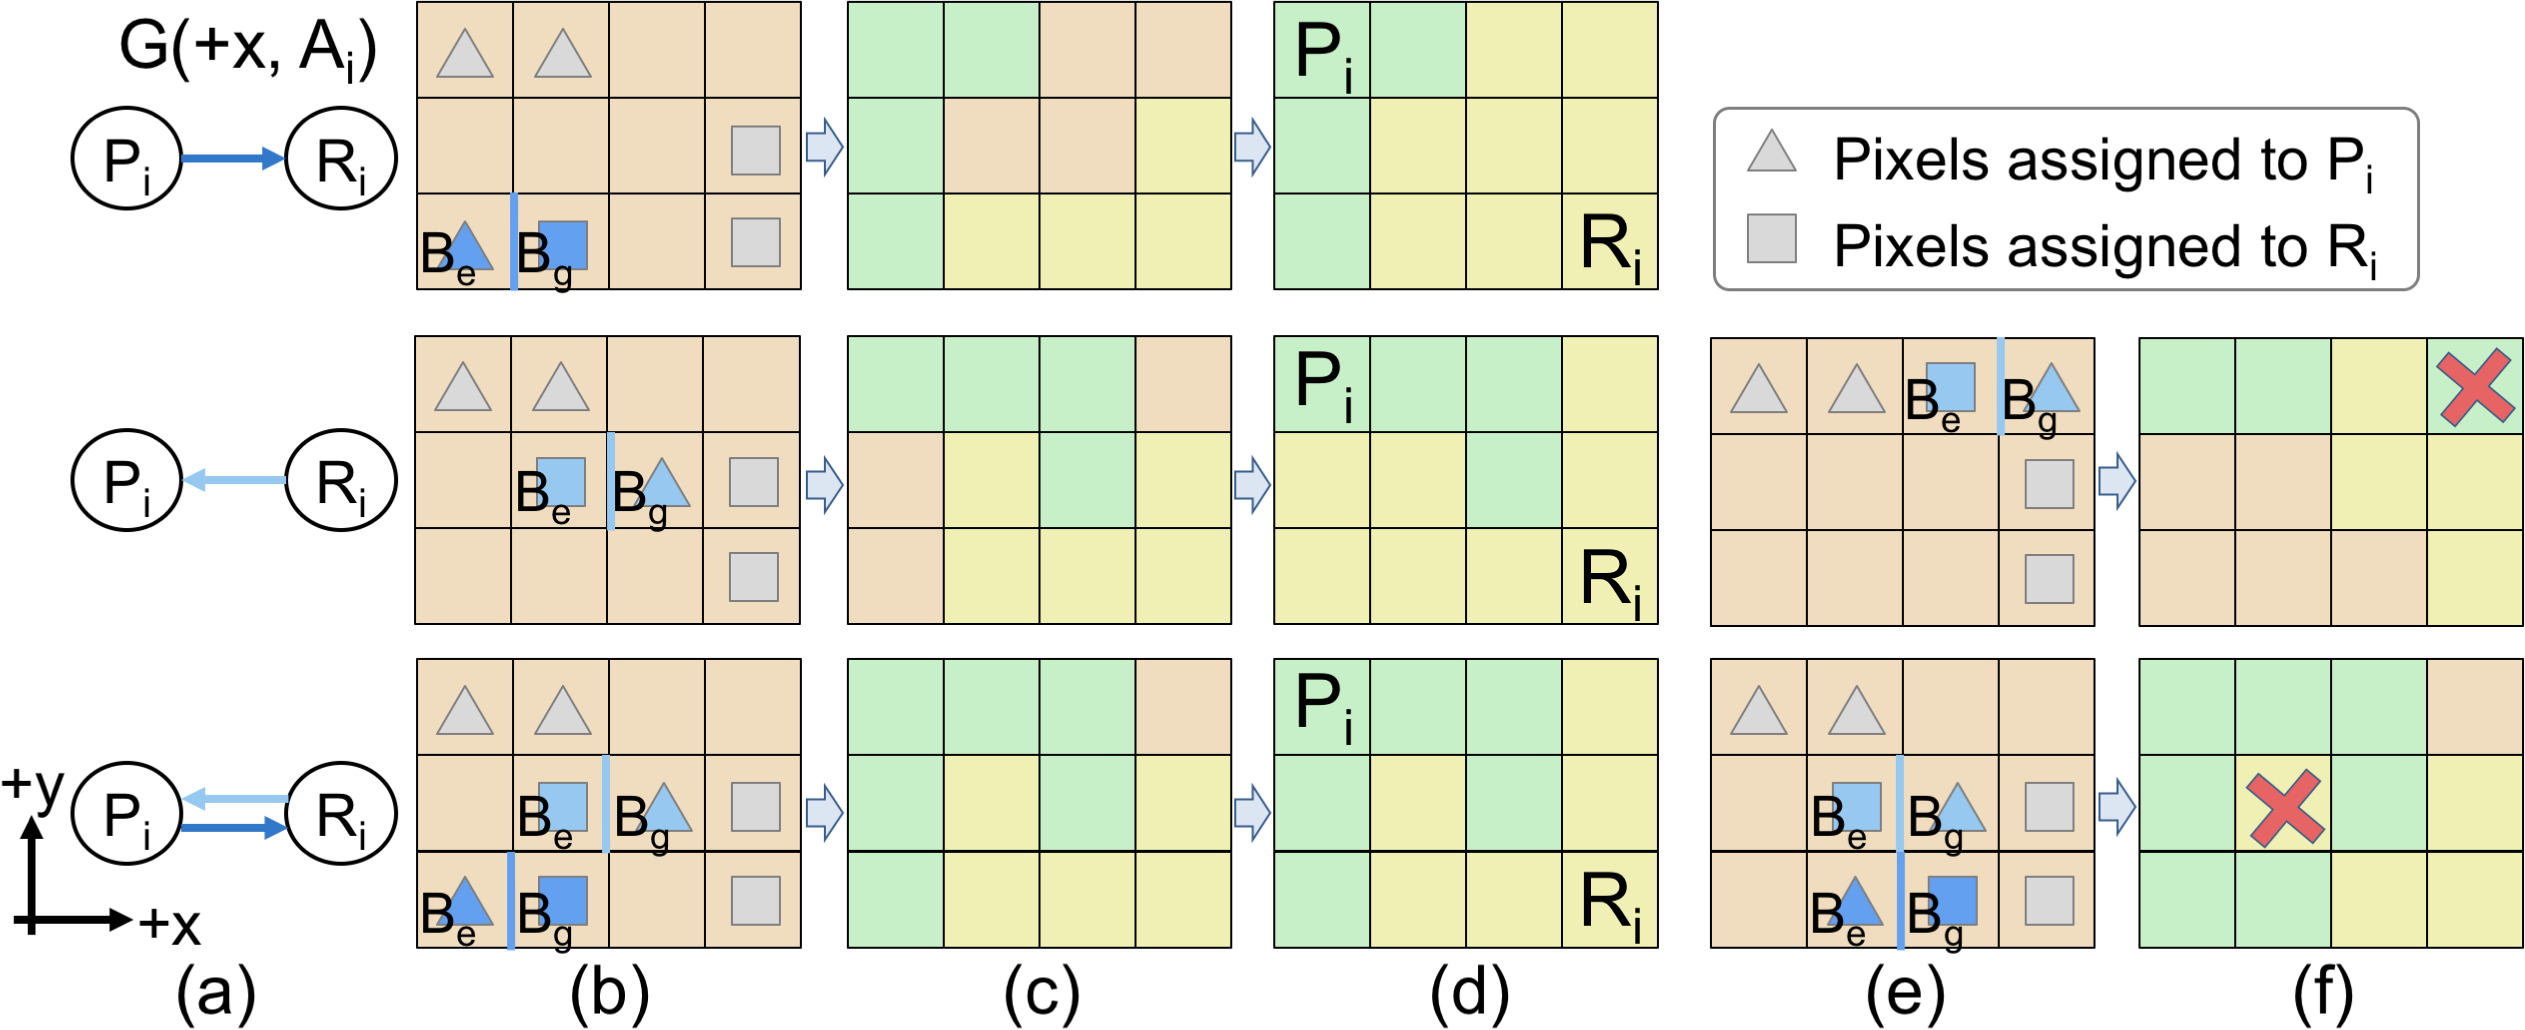
\includegraphics[width=8.45cm]{images/Framework_Blocking.png}
	\vspace*{-2.5mm}
	\caption{
		(a) Internal blocking relations between $P_i$ and $R_i$ in $G(+x, A_i)$.
		(b) Find blocking and blockee pixel in $R_{i-1}$ (in orange) according to the blocking relations.
		Blocking pixels and blockee pixels in (b) and their associated blocking relation in (a) are colored the same (light or dark blue).
		(c) Initial geometry of $P_i$ and $R_i$.
		(d) Final geometry of $P_i$ and $R_i$.
		(e\&f) Two failure examples due to disconnectivity of $P_i$ or $R_i$ (see the red cross).}
	%\vspace*{-4.5mm}
	\label{fig:Framework_Blocking}
\end{figure}

\begin{figure*}[!t]
	\centering
	%\vspace*{-3.5mm}
	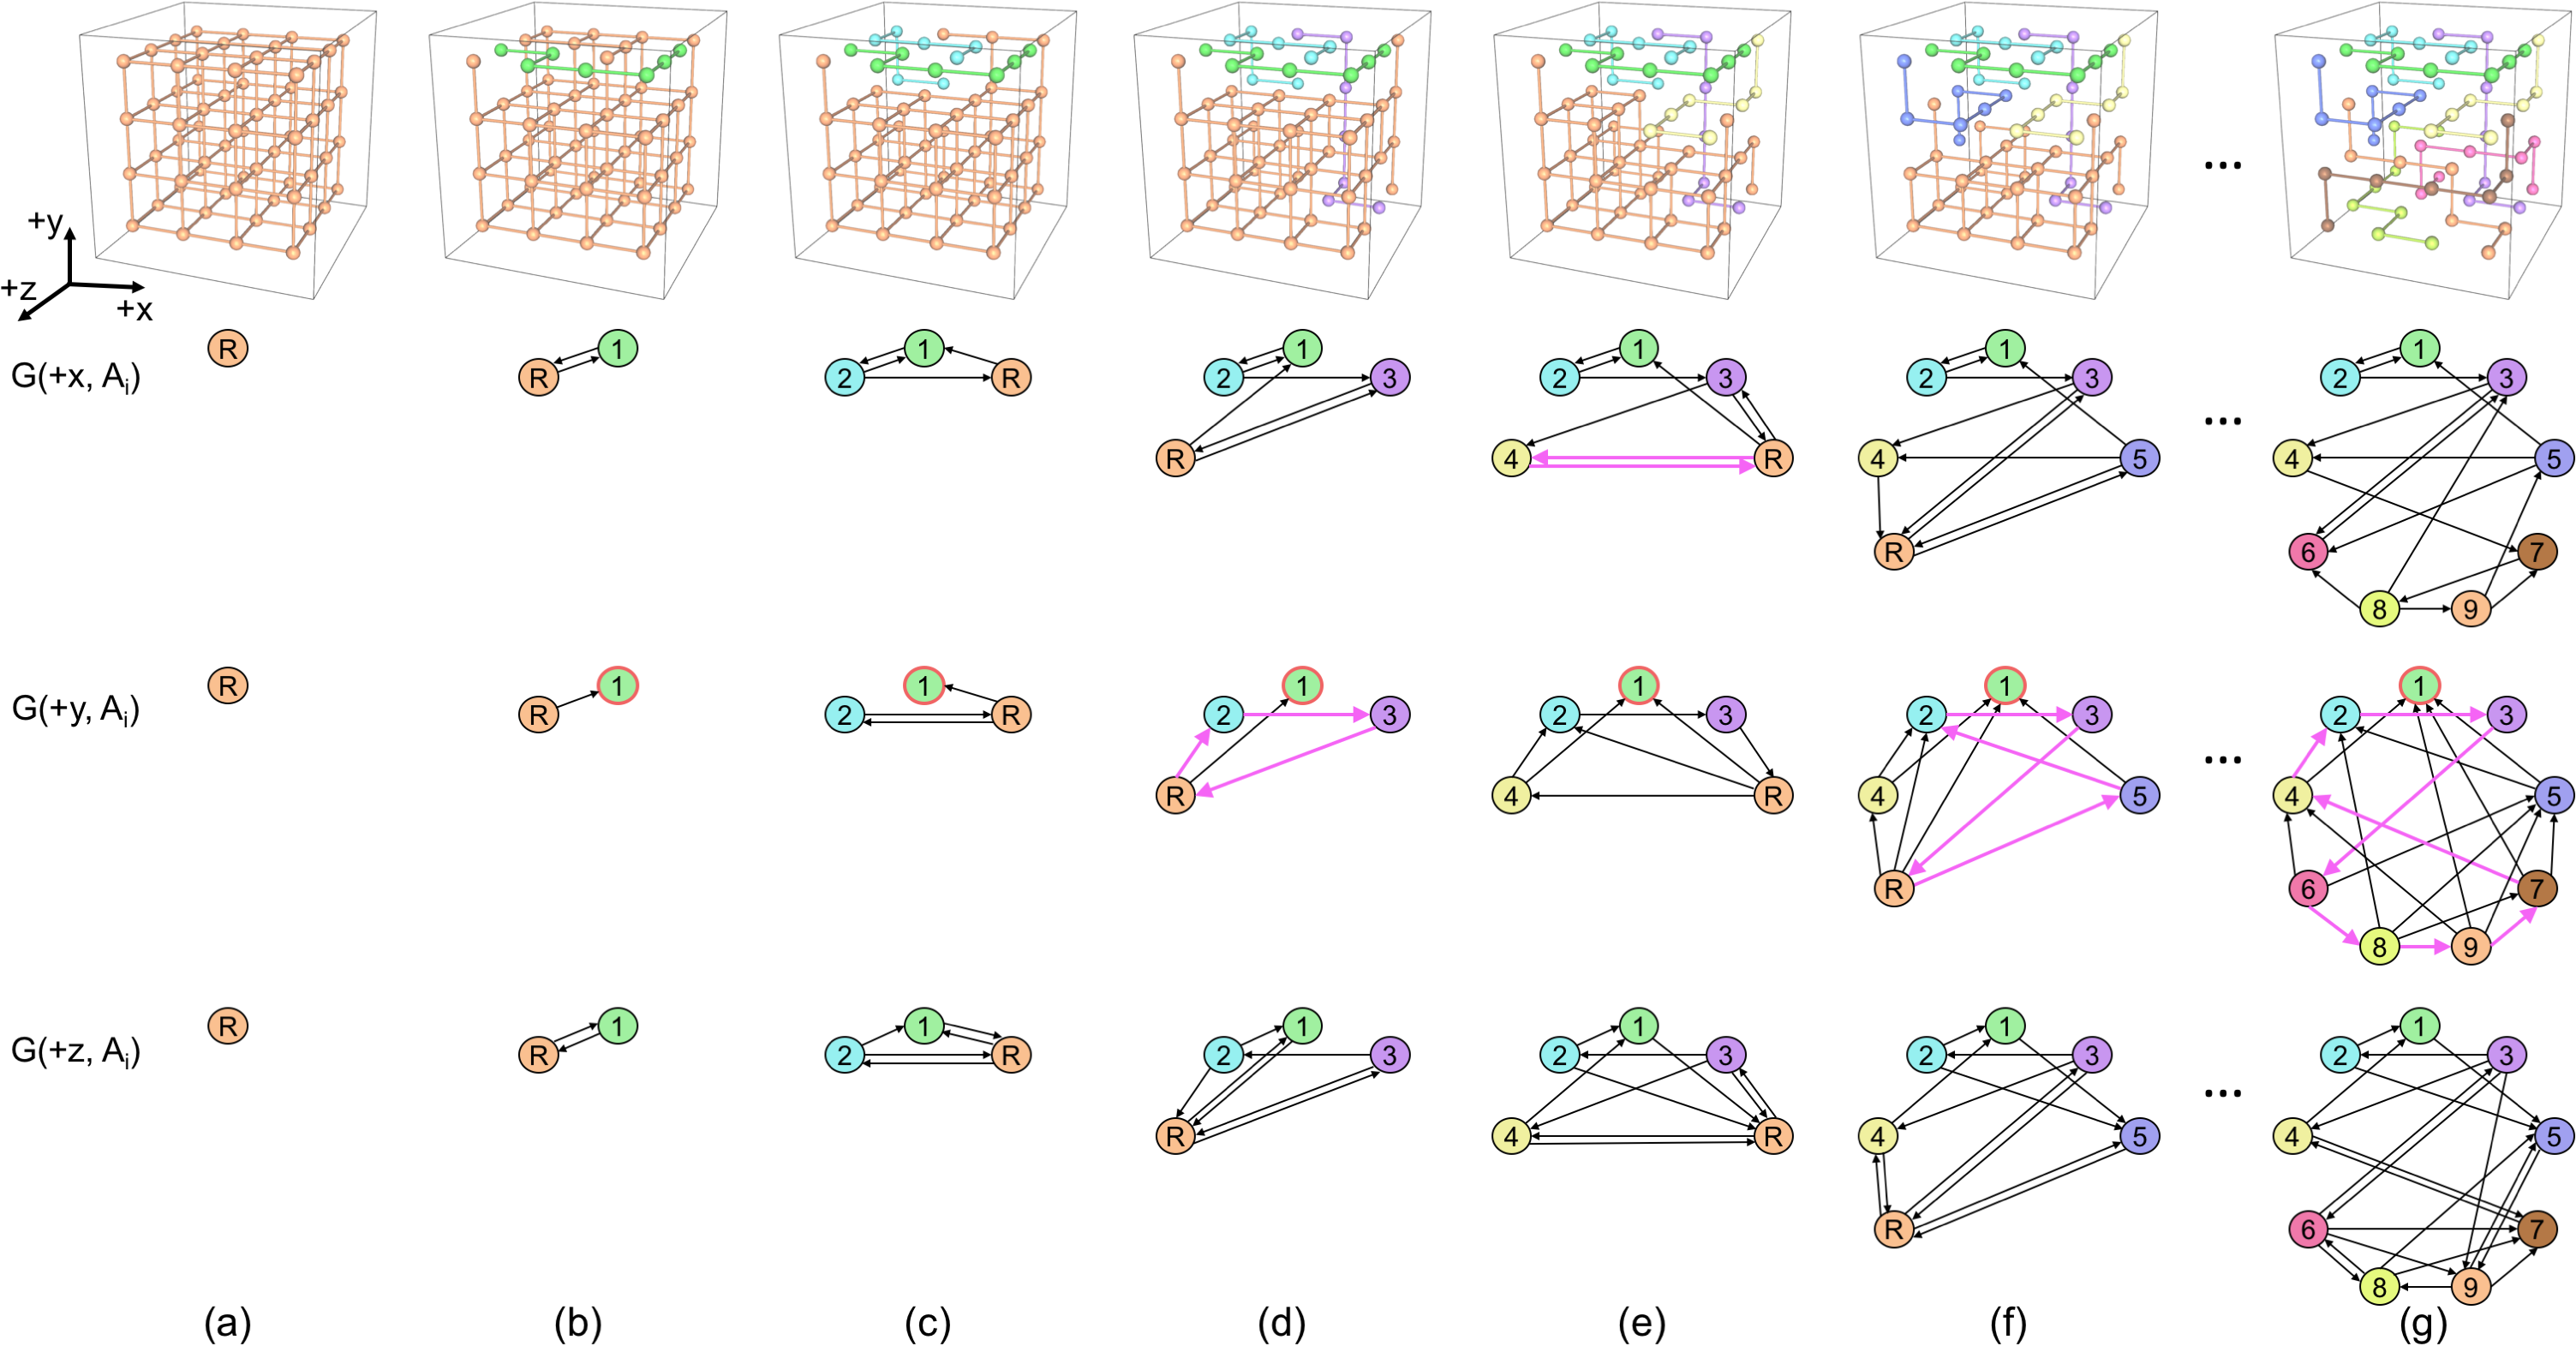
\includegraphics[width=17.7cm]{images/Application_Puzzle_Cube.png}
	\vspace*{-3.5mm}
	\caption{(a) Starting from a 4$\times$4$\times$4  voxel grid , (b-f) our framework iteratively construct the assembly pieces to create (g) a 9-piece interlocking {\textsc{Cube}}.
		Three DBGs are drawn for each intermediate assembly at the bottom.
		% where $P_i$ ($R_i$) are numbered as $i$ ($i+1$) in the DBGs. 
		Our approach allows immobilizing $P_i$ and $R_i$ by constructing cycles of various sizes (examples colored in purple).
		%The number of edges in the DBGs of~\cite{Song-2012-InterCubes} (21, 19, and 19, from top to bottom) is larger than (n) those of ours (14, 18, and 16, from top to bottom).	
		%This is because our approach allows constructing larger cycles to immobilize $P_i$ and $R_i$ (compare the cycles colored in purple in (d\&k) and (g\&n)).
		%The cycles (colored in purple) constructed to immobilize $P_4$ and $R_4$ have (d) 3 and (k) 4 parts respectively while those to immobilize $P_7$ and $R_7$ have (d) 3 and (k) 6 parts respectively.
	}
	\vspace*{-2.0mm}
	\label{fig:Application_Puzzle_Cube}
\end{figure*}


\vspace*{1.0mm}
\noindent
{\bf Geometry Realization of $P_i$ and $R_i$.}  \
%Now, a conceptual design of $P_i$ and $R_i$ has been represented as  a set of new directed edges in the base DBGs $\{G(d, A_i)\}$.
In order to realize $\{G(d, A_i)\}$ $\in \mathbf{C}_i$ in the embedded geometry, 
we perform the following steps, each corresponding to a counterpart of the graph design stage:
%, which can be customized for designing different kinds of interlocking assemblies.
%Here, we take 2D interlocking puzzle design as an example for illustration.
%\Mark{describe the correspondence between conceptual design and geometric realization}

\vspace*{1.0mm}
\noindent
{\em i) Identify external geometric contacts between $\{P_1, ..., P_{i-1}\}$ and $R_{i-1}$. } \
Recall that a directed edge $e_{i \rightarrow j}$ from $P_i$ to $P_j$ in $G(d, A)$ means that $P_j$ blocks the translation of $P_i$ along $d$.
This indicates that $P_i$ contacts $P_j$ along $d$, and $P_j$ locates further than $P_i$ along $d$; see again Figure~\ref{fig:NDBG}.
In an assembly $\mathbf{A}_{i-1}$, we identify such blocking contacts between $P_l$ ($1\leq l\leq{i-1}$) and $R_{i-1}$ for each base direction $d$ by computing the overlap of the respective boundaries along $d$ ($-d$), see Figure~\ref{fig:Framework_Geometry}(a\&b).



\vspace*{1.0mm}
\noindent
{\em ii) Distribute external geometric contacts. } \
An external blocking relation, say between $P_l$ and $R_{i-1}$,  in a DBG $G(d, A_{i-1})$ can be distributed to $P_i$, $R_i$, or both.
For the first two cases, the corresponding geometric contacts need to be totally assigned to $P_i$ or $R_i$ respectively; see Figure~\ref{fig:Framework_Geometry}(f).
For the last case, the geometric contacts need to be partitioned into two subsets and assigned to $P_i$ and $R_i$ separately; see Figure~\ref{fig:Framework_Geometry}(c).

However, this step could fail for two reasons.
First, the external geometric contact could be too small to be partitioned.
For example, $R_2$ contacts $P_2$ along $+y$ in a single pixel in Figure~\ref{fig:Framework_Geometry} (b).
Yet, this single pixel (marked with a red circle) needs to be assigned to both $P_3$ and $R_3$ in Figure~\ref{fig:Framework_Geometry}(d) according to the computed blocking relations, which is not feasible.
Second, the assignment of geometric contacts may conflict with one another across multiple DBGs.
For example, two pixels marked with red circles in Figure~\ref{fig:Framework_Geometry}(c) need to be assigned to $R_3$ to realize $G(+x, A_3)$.
However, these two pixels also need to be assigned to $P_3$ to realize $G(+y, A_3)$ in Figure~\ref{fig:Framework_Geometry}(e), leading to a conflict. 
 
\vspace*{1.0mm}
\noindent
{\em iii) Construct internal geometric contacts. } \
If $G(d, A_i)$ has $K\in \{1, 2\}$ internal blocking relations, we need to construct geometric contacts between $P_i$ and $R_i$.
Here, we take as an example the case of realizing a single directed edge from $P_i$ to $R_i$ to illustrate our approach; see Figure~\ref{fig:Framework_Blocking}(top).
Inspired by~\cite{Song-2012-InterCubes}, we find a pair of blocking and blockee pixels denoted as $B_g$ and $B_e$, respectively, which contact each other along $d$ among all unassigned pixels in $R_{i-1}$.
We then assign $B_e$ to $P_i$ and $B_g$ to $R_i$.
Other cases of realizing internal blocking relations can be handled similarly; see Figure~\ref{fig:Framework_Blocking}.

%Note that this step also could fail since we may not be able to find such a pair of blocking and blockee voxels, and/or the assignments of blocking and blockee voxels may make $[P_i, R_i]$ deadlocking or $R_i$ disconnected; see Figure~\ref{fig:Framework_Geometry}(d).

%There are generally four cases of creating internal blocking relations between $P_i$ and $R_i$ along $d$; see Figure~\ref{fig:Blocking_Relation}.

\vspace*{1.0mm}
\noindent
{\em iv) Construct initial parts geometry. } \
By now, we have identified all the pixels in $R_{i-1}$ that need to be assigned to $P_i$ or $R_i$ to make $\mathbf{A}_i$ interlocking.
%We further identify all pixels on top of $P_i$ along $d$ to $P_i$ such that $P_i$ is separable from $R_i$ in $[P_i, R_i]$ along $d$; see the pixel with a pink marker in Figure~\ref{fig:Framework_Geometry}(h).
To form an initial $P_i$ ($R_i$), we connect these pixels into a single part using the shortest path; see Figure~\ref{fig:Framework_Geometry}(h) and~\ref{fig:Framework_Blocking}(c).
Note that this connection process can fail since we may not be able to find such a shortest path without disconnecting parts; see Figure~\ref{fig:Framework_Blocking}(e\&f) for examples.

\vspace*{1.0mm}
\noindent
{\em v) Ensure disassemblability. } \
To make $P_i$ movable in $[P_i, R_i]$, we first identify all possible moving directions of $P_i$ in $\{G(d, A_i)\}$, i.e., the directions where $P_i$ is unblocked by $R_i$; e.g.,  $P_3$ could be movable along $\{-x, +x, +y\}$ in $[P_i, R_i]$ according to the blocking graph in Figure~\ref{fig:Framework_Geometry}(c\&g) .
We try each possible moving direction of the initial $P_i$ and discard those that cannot be achieved in the embedded geometry. 
%e.g., $P_i$ seems movable along $+x$ in Figure~\ref{fig:Framework_Blocking}(middle; a) according to the conceptual design yet it cannot really move along $+x$ due to blocking of $R_i$ in Figure~\ref{fig:Framework_Blocking}(middle; b\&c).
We consider that $P_i$ is disassemblable in $[P_i, R_i]$ if we can find one movable direction of $P_i$, along with a disassembly path.
Lastly, we assign those remaining pixels in $R_{i-1}$ (see orange pixels in Figure~\ref{fig:Framework_Blocking}(c)) to $P_i$ and $R_i$ respectively according to geometric proximity (with preference to $R_i$), while maintaining the disassemblability of $P_i$ in $[P_i, R_i]$; see Figure~\ref{fig:Framework_Geometry}(i) and~\ref{fig:Framework_Blocking}(d).

A graph design is realized if all above steps succeed. Otherwise, we discard this design and try another one in $\mathbf{C}_i$. If all candidates in $\mathbf{C}_i$ fail, we backtrack to the other nodes in the construction tree following the procedure in Algorithm~\ref{alg:Alg_Framework}.


%\Mark{In the above paragraphs and figures, we frequently mention failure case, but we do not state how we handle them. We should state very clearly what happens if one step fails!}

%\Mark{In general, the above explanation is very descriptive, i.e. it explains the steps of the algorithm, but it does not necessarily explain, why this is the only/right approach to take. It might help to have a high-level overiew, maybe some pseudo-code or diagram, to provide a big-picture view of the method.}

%\Mark{It might also not be clear how representative the puzzle example is. It's good to explain the algorithm, but is it obvious how other cases are treated, i.e. will readers understand that this in indeed a general approach? Maybe a forward reference to the next section would be helpful.}

%Note that this step also could fail since the assignment of voxels could make $[P_i, R_i]$ deadlocking and/or or $R_i$ and/or disconnected; see Figure~\ref{fig:Framework_Geometry}(d).

%This is achieved by properly assigning remaining geometry in $R_{i-1}$ to $P_i$ or $R_i$; see Figure~\ref{fig:Framework_Geometry}(i) for an example. %\Peng{may need more details here.}



%%%%%%%%%%%%%%%%%%%%%%%%%%%%%%%%%%%%%%%%%%%%%%%%%%%%%%%%%%%%%%%%%%%%%%%%%%%%%%%%%%%%%%%%%%%%%%%%%%%
% Backup
%%%%%%%%%%%%%%%%%%%%%%%%%%%%%%%%%%%%%%%%%%%%%%%%%%%%%%%%%%%%%%%%%%%%%%%%%%%%%%%%%%%%%%%%%%%%%%%%%%%









%%%%%%%%%%%%%%%%%%%%%%%%%%%%%%%%%%%%%%%%%%%%%%%%%%%%%%%%%%%%%%%%%%%%%
% Overivew
%%%%%%%%%%%%%%%%%%%%%%%%%%%%%%%%%%%%%%%%%%%%%%%%%%%%%%%%%%%%%%%%%%%%


\section{Results and Discussion}
\label{sec:results}

In this section we show how our framework can be used for designing various kinds of interlocking assemblies, with example applications as puzzles, furniture, sculptures, or architectural designs. We highlight differences to previous approaches to show how our method improves the state of the art and enables new kinds of interlocking assemblies not possible before. For more detailed comparisons and results we refer to the supplementary material.

%%%%%%%%%%%%%%%%%%%%%%%%%%%%%%%%%%%%%%%%%%%%%%%%
% 1. Interlocking Puzzle
%%%%%%%%%%%%%%%%%%%%%%%%%%%%%%%%%%%%%%%%%%%%%%%%

\begin{figure*}[!t]
	\centering
	%\vspace*{-3.5mm}
	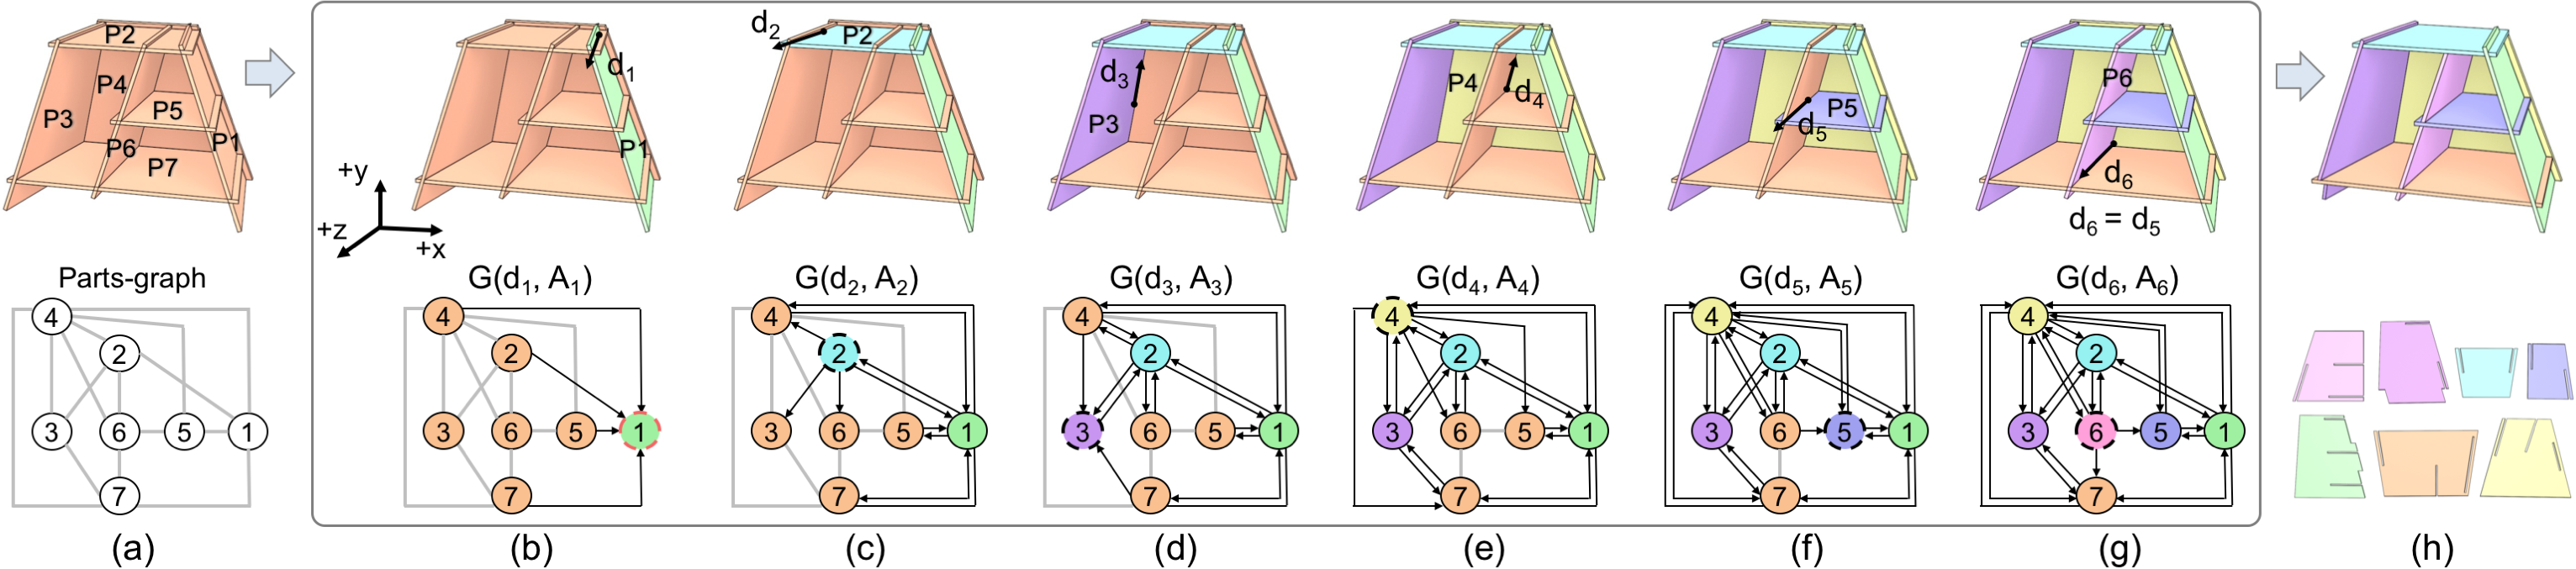
\includegraphics[width=17.75cm]{images/Application_Plate_Cabinet.png}
	\vspace*{-3.5mm}
	\caption{Design of a 7-part interlocking \textsc{Cabinet} by our approach.
		(a) Input design and parts-graph.
		(b-g) The iterative procedure to plan the joints, where the removal direction $d_i$ of $P_i$ is shown in the top and
		the active DBG $G(d_i, A_i)$ is shown at the bottom.
		All orange nodes in each DBG form $R_i$ and the node with dashed boundary is $P_i$.
		(h) The interlocking result and the parts.}
	\vspace*{-2.0mm}
	\label{fig:Application_Plate_Cabinet}
\end{figure*}

\subsection{Interlocking Voxelized Structures}
\label{subsec:puzzle}

Given a voxelized shape and a desired number of parts $N$ as input, our goal here is to decompose the voxel set into a collection of parts that form an interlocking assembly~\cite{Song-2012-InterCubes}.
Figure~\ref{fig:Application_Puzzle_Cube} shows our iterative design process for creating a 9-piece $4\times 4 \times 4$ interlocking {\textsc{Cube}}.
%Our approach have been detailed in Section~\ref{sec:approach}.
%Note that our approach cannot create puzzles with large $N$ may from an input model with relatively small number of voxels.
%For example, our approach cannot find a 10-piece $4\times 4 \times 4$ interlocking {\textsc{Cube}}.

The major difference between our approach and~\cite{Song-2012-InterCubes} is the graph design of $P_i$ and $R_i$ to ensure interlocking of $\mathbf{A}_i$. Our approach makes use of all previous pieces $\{P_1, ..., P_{i-1}\}$ to immobilize $P_i$ and $R_i$.  (i.e., form a cycle in each $\{G(d, A_i)\}$; see Figure~\ref{fig:Framework_Cycle} and~\ref{fig:Application_Puzzle_Cube}), while~\cite{Song-2012-InterCubes} only relies on $P_{i-1}$ to immobilize $P_i$ and $R_i$ (i.e., form a 2-part or 3-part cycle in the DBGs; see Figure~\ref{fig:Application_Puzzle_Model}).
Note that our approach can easily generate recursive interlocking puzzles as~\cite{Song-2012-InterCubes} by constraining our graph design as shown in Figure~\ref{fig:Application_Puzzle_Model}.

\begin{figure}[!t]
	\centering
	%\vspace*{-3.5mm}
	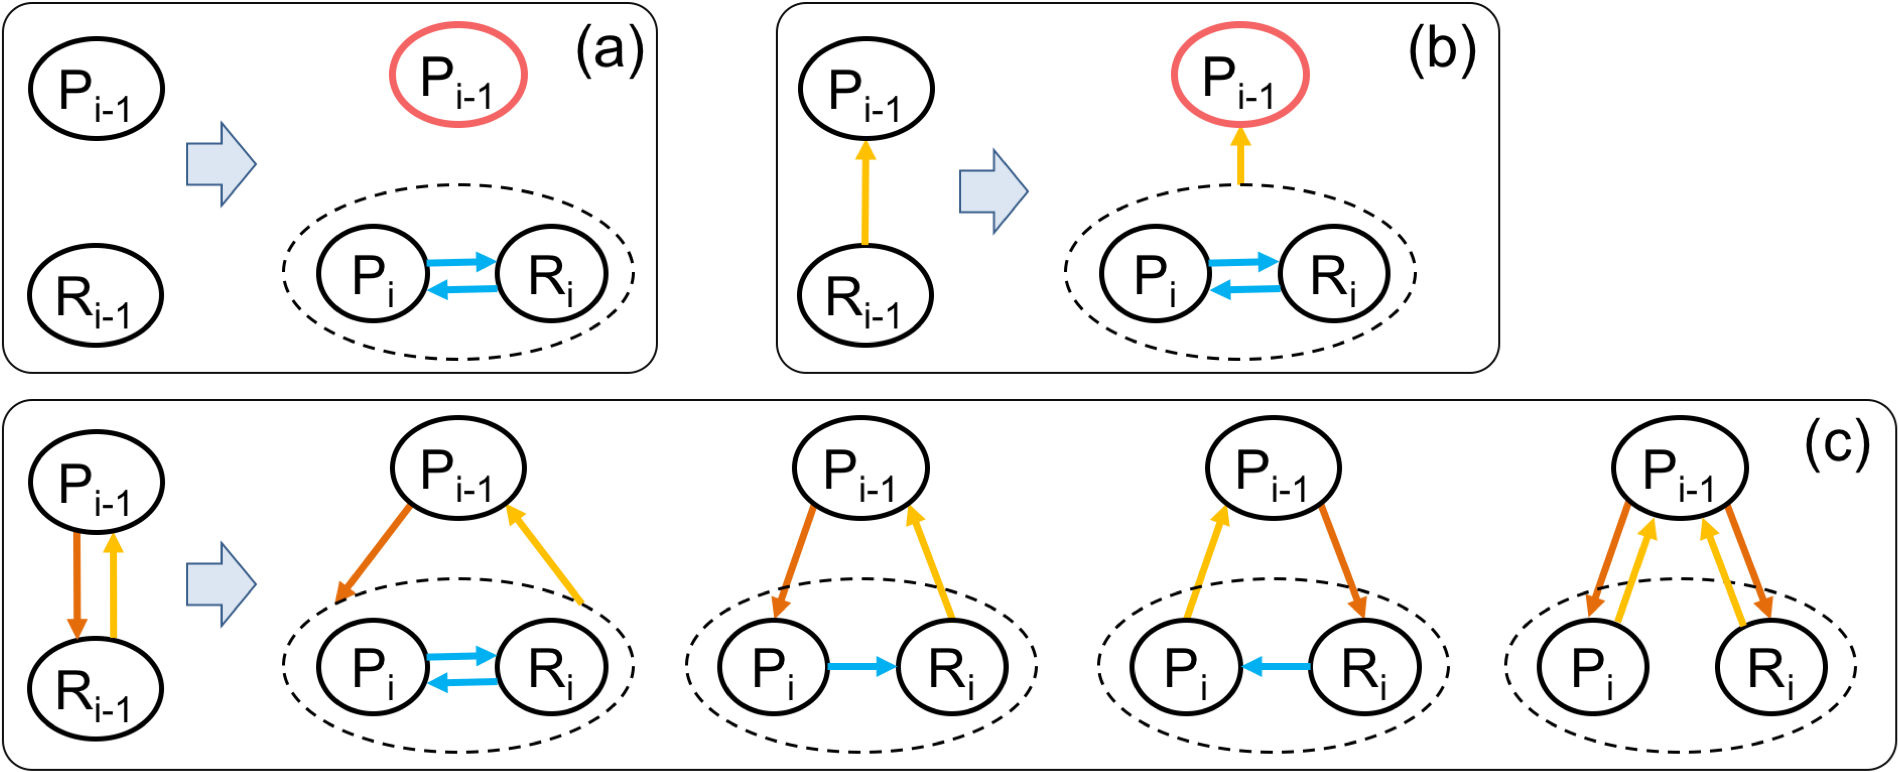
\includegraphics[width=8.40cm]{images/Application_Puzzle_Model.png}
	\vspace*{-2.5mm}
	\caption{
		Illustration of the model of~\cite{Song-2012-InterCubes} based on our DBG-based representation. This approach achieves global interlocking of $A_n$ by requiring every $[P_{i-1}, P_i, R_i]$ ($2 \leq i\leq n$) to form a local interlocking group with $P_{i-1}$ as the key.
		In detail, $P_{i-1}$ and $R_{i-1}$ in $G(d, A_{i-1})$ are possible to have (a) zero, (b) one, and (c) two directed edges.
		%(a) This case is not supported in~\cite{Song-2012-InterCubes} since every part is movable in $[P_{i-1}, P_i, R_i]$ and the approach cannot use any other existing $P_j$ to create blocking relations; 
		%after the partitioning of $R_{i-1}$;
		(a\&b) $P_i$ and $R_i$ are immobilized in a 2-part cycle $[P_i, R_i]$;
		% while the local key $P_{i-1}$ is movable along $d$ in $[P_{i-1}, P_i, R_i]$.
		(c) $P_i$ and $R_i$ are immobilized in either a 2-part cycle $[P_i, R_i]$, $[P_{i-1}, P_i]$, $[P_{i-1}, R_i]$, or a 3-part cycle $[P_{i-1}, P_i, R_i]$.
		%where the rightmost subcase will not happen since $P_i$ and $R_i$ should have at lease one edge.
	}
	\vspace*{-4.0mm}
	\label{fig:Application_Puzzle_Model}
\end{figure}




%Due to this reason, our designed puzzles are interlocking only at the final assembly state while those by~\cite{Song-2012-InterCubes} are interlocking at each intermediate assembly state (i.e., recursive interlocking).
%A good property of recursive interlocking puzzles is that they can be assembled with no or very few supports.
%On the other hand, this property results in strict constraint on the geometry realization, restricting the flexibility of designing interlocking puzzles. 
%

% since each piece locks the successive pieces. 
%\Mark{This could be interpreted as an advantage of your previous approach. It sounds like it would be better for assembly if all stages are interlocking. We should probably highlight the drawbacks of this again.}
%Recursive interlocking puzzles can be assembled with no or very few supports since each intermediate assembly of puzzle pieces remains steady due to interlocking.
 
%Figure~\ref{fig:Application_Puzzle_Cube} compares two 8-piece interlocking cubes designed by our approach and~\cite{Song-2012-InterCubes}, where our constructed cycles in the DBGs have much larger variations than those of~\cite{Song-2012-InterCubes}. 


\begin{figure}[!b]
	\centering
	\vspace*{-3.5mm}
	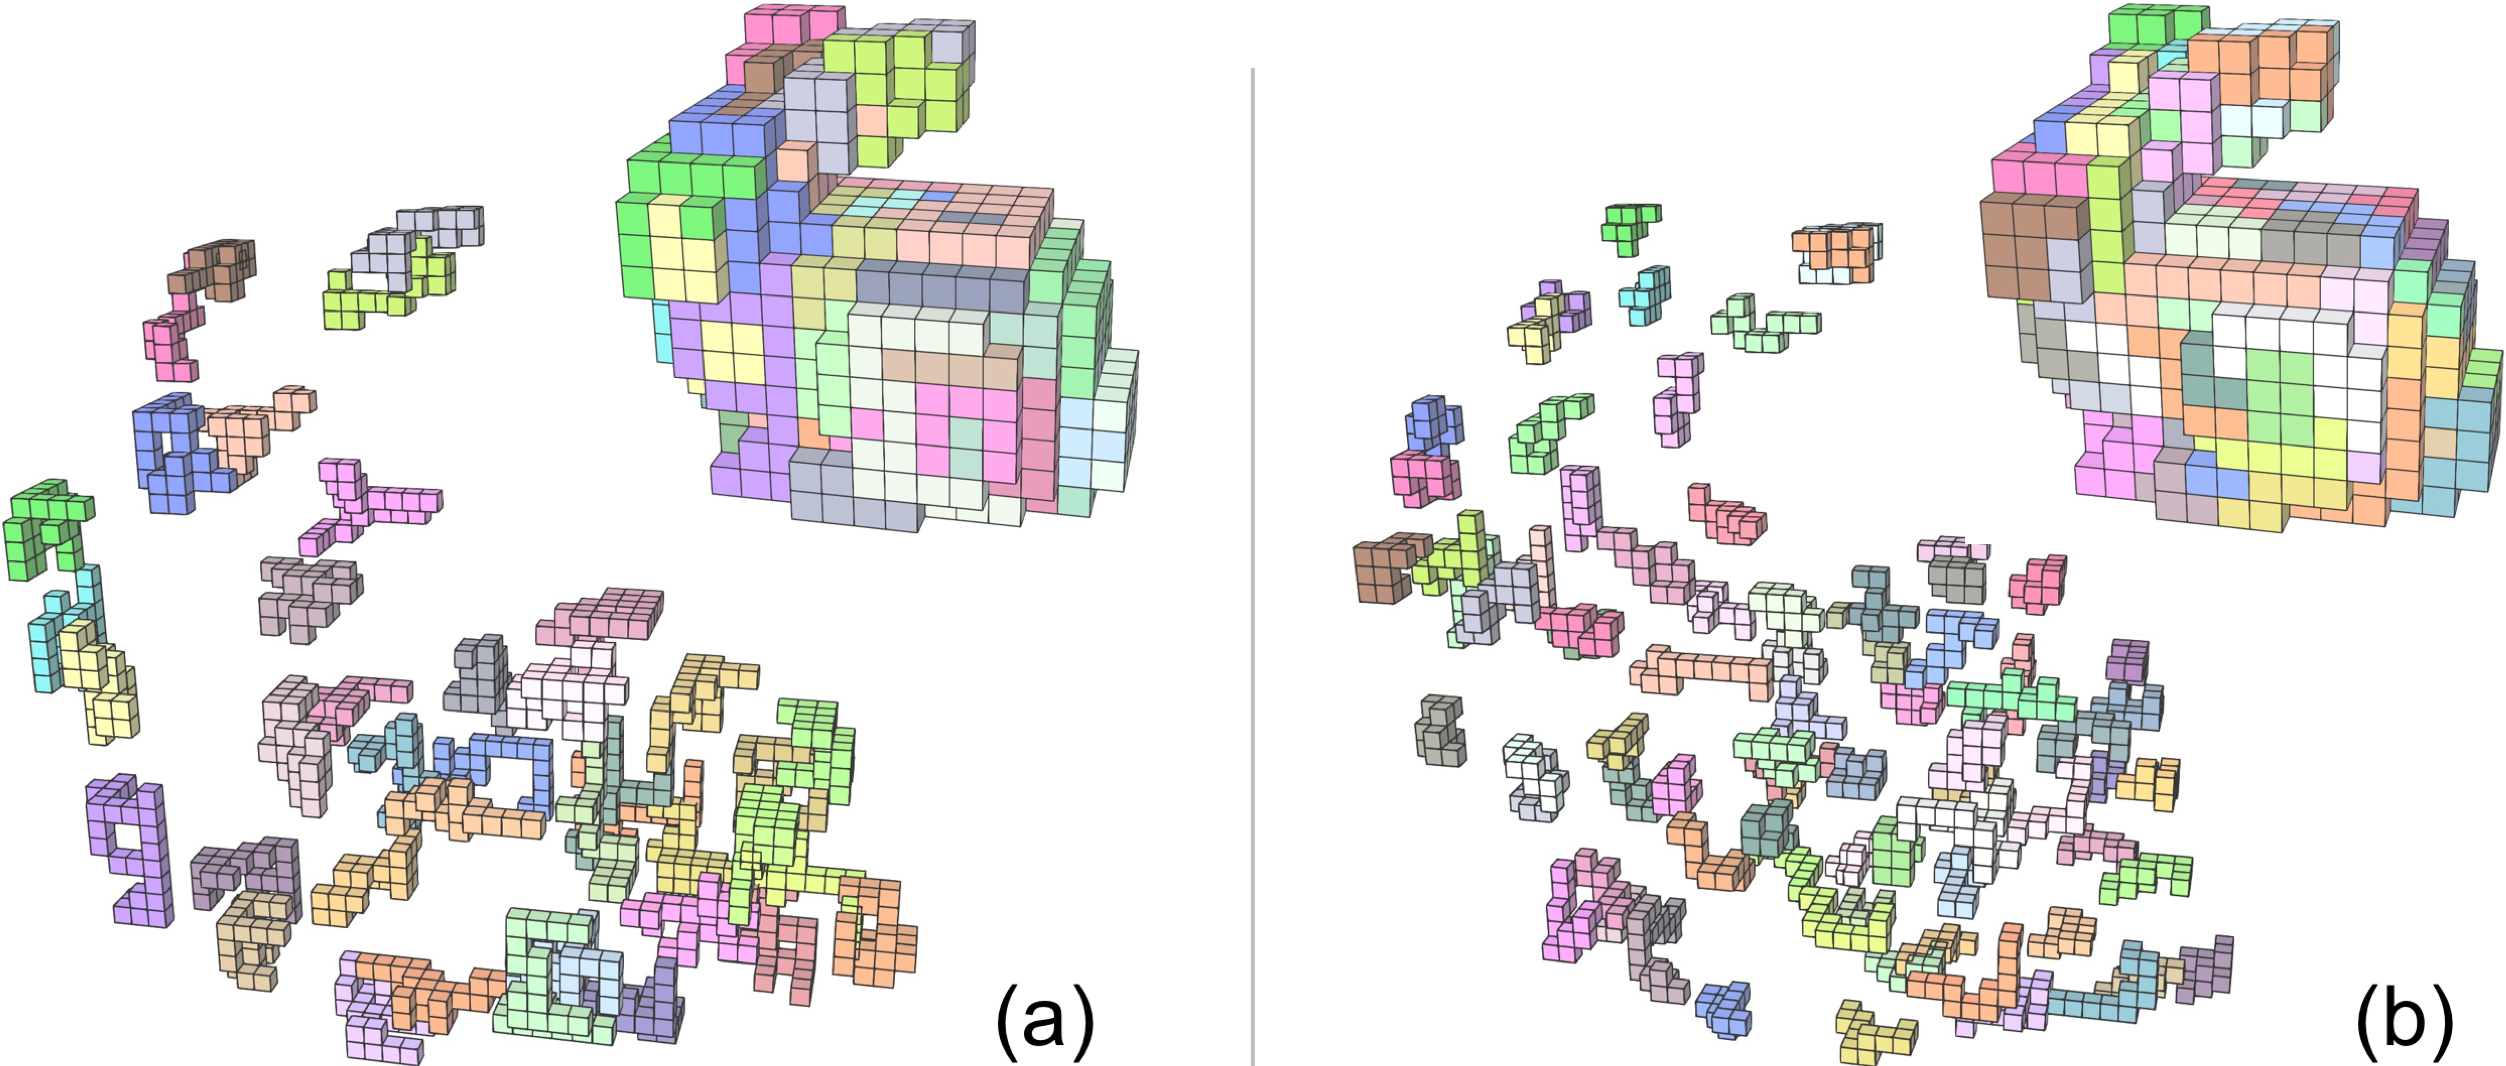
\includegraphics[width=8.20cm]{images/Result_Puzzle_Bunny.png}
	\vspace*{-2.5mm}
	\caption{
		Interlocking {\textsc Bunny}s  (966 voxels). Our method can find assemblies with a large number of parts:  (a)  maximally 40 pieces can be found by the method of~\cite{Song-2012-InterCubes}; (b) 80 pieces using our approach.	
		%Exploded puzzle pieces ($N=40$ in (a) and $N=80$ in (b)) are shown on the left.
	}
	%\vspace*{-4.0mm}
	\label{fig:Result_Puzzle_Bunny}
\end{figure}


%Song et al.~\shortcite{Song-2012-InterCubes} proposes an iterative approach to design recursive interlocking puzzles from a given voxelized shape, where the assembly of puzzle pieces (with at least three pieces) remains interlocking after the sequential removal of pieces.
%A formal model is proposed to ensure global interlocking of all extracted puzzle pieces (i.e., $A_i$) by enforcing local interlocking requirement on every three consecutive intermediate puzzle pieces (i.e., $[P_{i-1}, P_i, R_i]$).  

%We also iteratively construct the puzzle pieces as~\cite{Song-2012-InterCubes}.
% by partitioning each $R_{i-1}$ into $P_i$ and $R_i$.

However, exploiting all existing blocking relations to immobilize $P_i$ and $R_i$ provides significantly more degrees of freedom for designing interlocking assemblies. This allows us to incorporate additional design goals, for example on part appearance as for the {\textsc{Cartoon Dog}} in Figure~\ref{fig:teaser}. Here we impose constraints that avoid cutting seams across geometric features, so that eyes, ears, nose, and tail are each assigned to a single assembly piece.
In addition, as shown in Figure~\ref{fig:Result_Puzzle_Bunny}, our approach can find interlocking assemblies with significantly more parts than~\cite{Song-2012-InterCubes} for the same input.




%First, our approach can generate a significantly larger number of conceptual designs that can be tried at the geometric realization stage.
%This significantly reduces constraint on the geometric realization of the pieces, making it possible to generate interlocking results that cannot be achieved by~\cite{Song-2012-InterCubes}.



%%%%%%%%%%%%%%%%%%%%%%%%%%%%%%%%%%%%%%%%%%%%%%%%
% 2. Interlocking Furniture
%%%%%%%%%%%%%%%%%%%%%%%%%%%%%%%%%%%%%%%%%%%%%%%%


\subsection{Interlocking Plate Structures}
\label{subsec:furniture}

% Problem formulation
%Our framework can be used to design interlocking furniture, in which parts interlock with one another to form a steady assembly.
%Our input is a furniture design represented as a set of simple 3D parts, where adjacent parts may contact or intersect.
%Our goal is to make the furniture interlocking by planning a network of joints between adjacent parts and further modifying the 3D parts with appropriate joint geometry accordingly.
%Similar to~\cite{Fu-2015-Furniture},  we consider parts that are orthogonally connected, and joints that connect a pair of parts and restrict each part to move along a specific axial direction;  see Figure~\ref{fig:Joints}.

 \begin{figure}[!t]
	\centering
	%\vspace*{-3.5mm}
	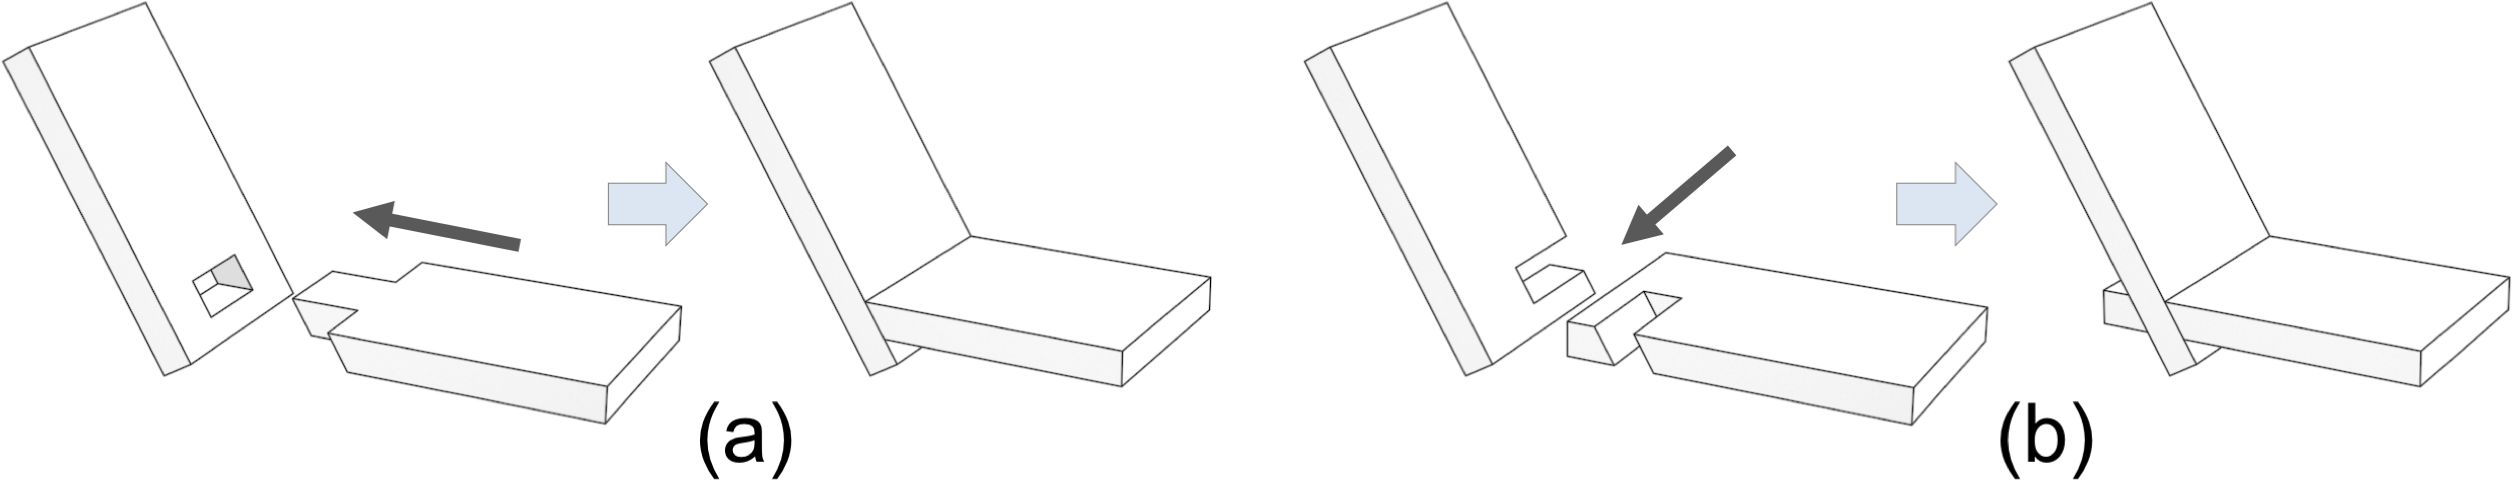
\includegraphics[width=8.45cm]{images/Application_Plate_Joints.png}
	\vspace*{-2.5mm}
	\caption{Variants of (a) mortise-and-tenon joints and (b) halved joints that support non-orthogonal part connection with surface contact.
		%\Mark{Shouldn't we just use (a) and (b)? No need to separate the figures more, I think.}
		%The green arrow shows the possible moving direction of the blue part.
	}
	\vspace*{-4.0mm}
	\label{fig:Application_Plate_Joints}
\end{figure}
 
A second class of assemblies that we can create with our approach are interlocking plate structures that have applications in furniture design or architecture, for example.
These assemblies differ in two main ways from the voxelized assemblies described above.
First, the geometry of parts and their connections are predefined. We model part connections with an undirected {\em parts-graph}, in which nodes represent parts, and edges connect two contacting/intersecting parts; see Figure~\ref{fig:Application_Plate_Cabinet}(a). 
Blocking relations can only be constructed between parts connected in the parts-graph.
The dual of a {\em parts-graph} is a {\em joints-graph}, where nodes represent joints and edges represent parts; see Figure~\ref{fig:Application_Frame_Cube}(a). 
Second, we use a set of predefined joint geometries to impose blocking relations between each pair of adjacent parts in the structure. 
Specifically, we consider mortise-and-tenon, halved, and dovetail joints that restrict each part to move along a single direction; see Figure~\ref{fig:Joints}.
To support non-orthogonal part connection, we consider suitable variants of mortise-and-tenon and halved joints;
\setlength{\columnsep}{12pt}
\begin{wrapfigure}{r}{0.32\columnwidth}
	\vspace{-12pt}
	\centering
	\hspace{-8pt}
	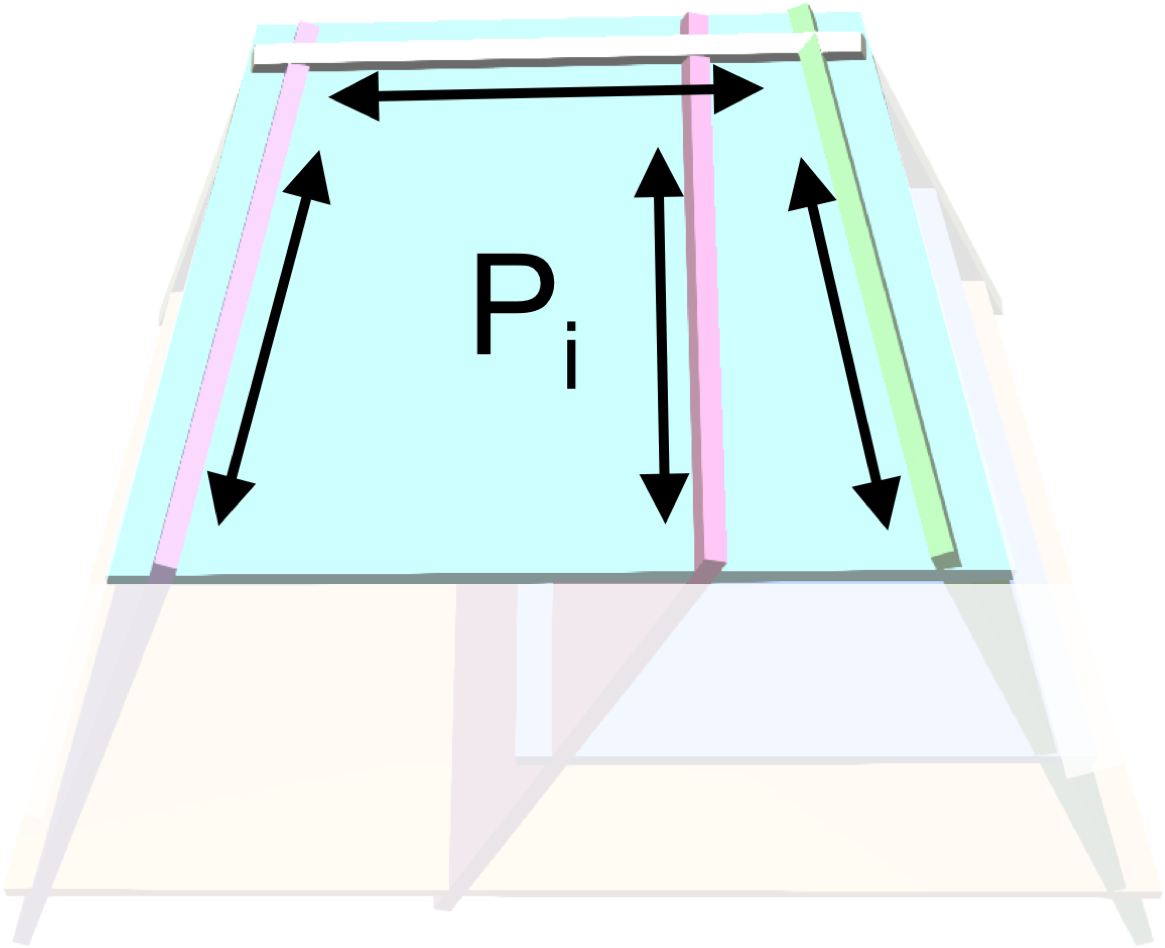
\includegraphics[width=0.30\columnwidth]{images/Application_Plate_Direction.png}
	\vspace{-11pt}
\end{wrapfigure}
see Figure~\ref{fig:Application_Plate_Joints}.
In plate structures,  the edge vectors shared between each part $P_i$ and its adjacent parts indicate the base directions $\{d\}$ (see the arrows in the inset for examples), which degenerate into six axial directions for structures where parts are orthogonally connected; see Figure~\ref{fig:Application_Furniture_Table}(a).

\if 0
To address above specifics of interlocking plate structures, we have the following adaptations to our framework.
First, we iteratively select a single part $P_i$  from the input, and consider the set of unselected parts as $R_i$.
At each iteration, our goal is to select a part from $R_{i-1}$ as $P_i$ and choose a removal direction of $P_i$ in $[P_i, R_i]$ denoted as $d_i$ such that $\mathbf{A}_i$ ($i\geq$2) is interlocking. 
\fi

%For a non-orthogonal HV joint, the removal direction is $\vec{e}$, which is an edge vector shared between parts.
%And we may choose between $+\vec{e}$ and $-\vec{e}$ when planning the joint; see Figure~\ref{fig:Application_Plate_Joints}(a\&b).
%For a non-orthogonal MT joint, the removal direction $\vec{d_t}$ of the tenon part is perpendicular to the part's normal; see Figure~\ref{fig:Application_Plate_Joints}(c\&d).

%For a halved joint the removal direction is the vector shared between parts that can be chosen in either orientation when planning the joint. 
%For a mortise-tenon joint, the removal direction of the tenon part is perpendicular to the part's normal.

%which allow parts to be non-orthogonally connected along planar surfaces

%
% In the three base DBGs, planning a joint between $P_i$ and $P_j$ that restricts $P_i$ to move along $d_i$ relative to $P_j$ will create a directed edge between the two parts in $G(d_i, A)$ and two directed edges in the other two base DBGs.
 %
 % Customized framework
 %
 

 
 \begin{figure*}[!t]
 	\centering
 	%\vspace*{-3.5mm}
 	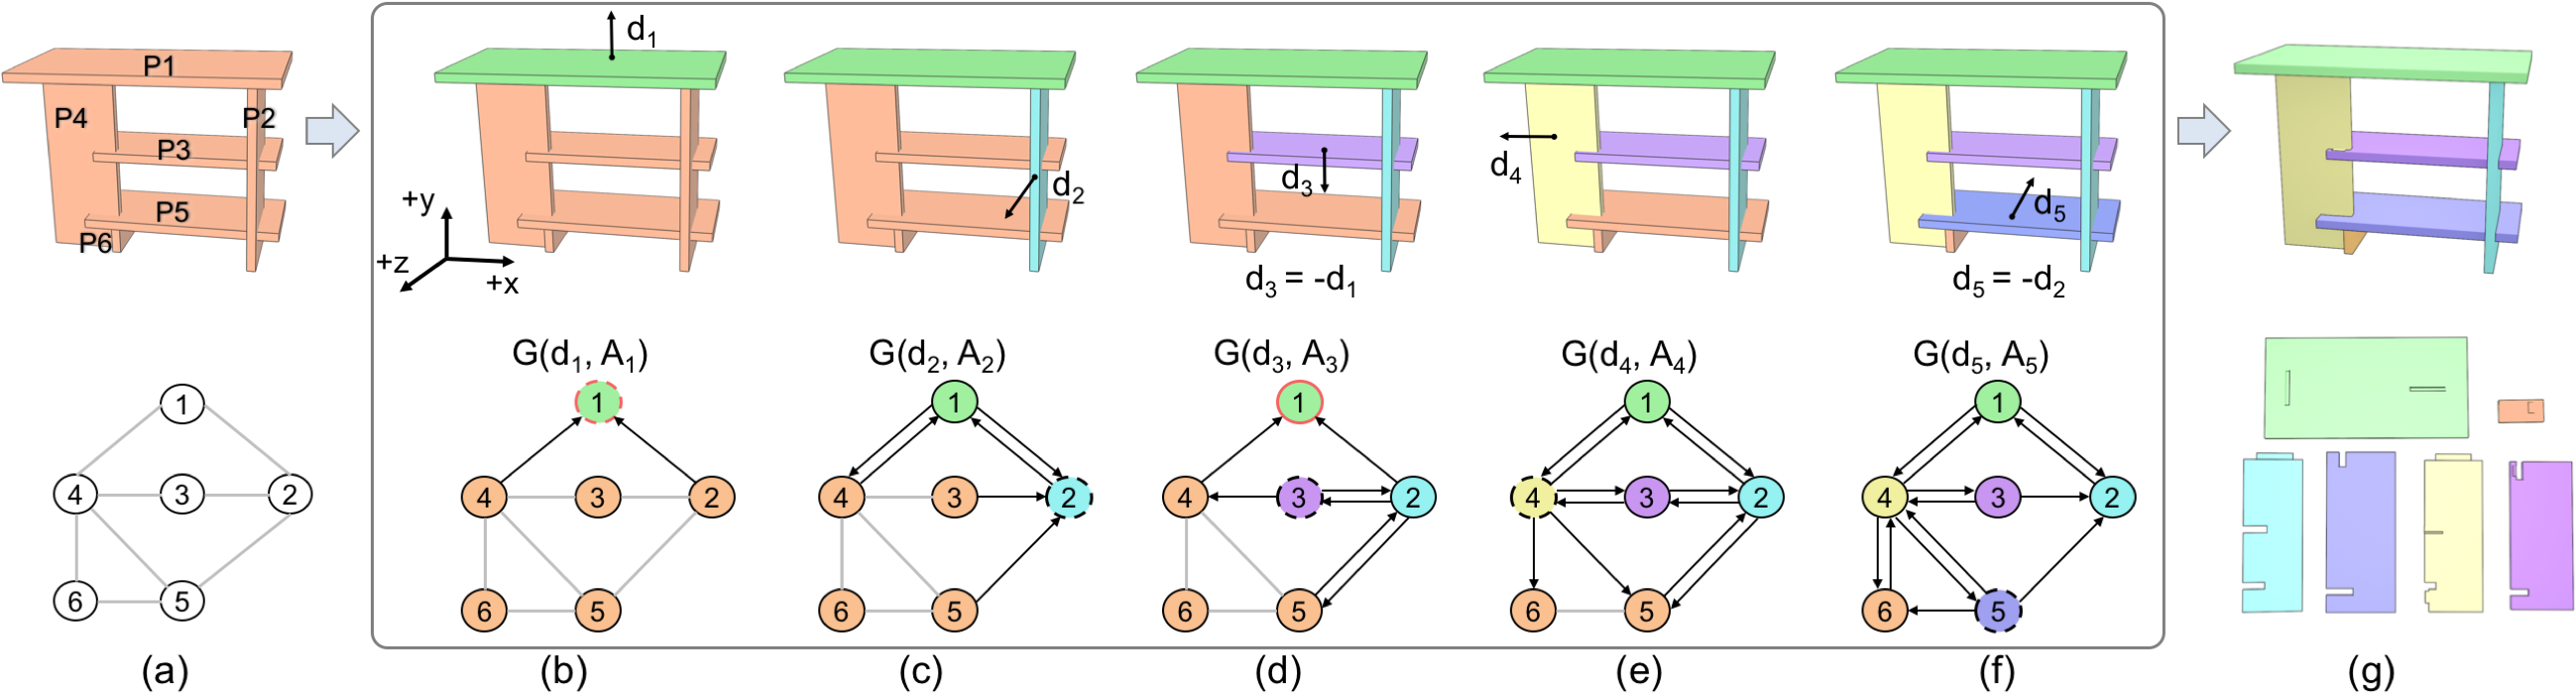
\includegraphics[width=17.75cm]{images/Application_Furniture_Table.png}
 	\vspace*{-3.5mm}
 	\caption{Design of a 6-part interlocking \textsc{Table} with orthogonal joints.
 		(a) Input design and parts-graph.
 		(b-f) The iterative procedure to plan the joints.
 		(g) The interlocking result and the parts.
 		%\Mark{I like this example for illustration. But people could argue that such a design, one could easily do by hand. We should also have examples where the complexity is to high to be able to figure things out manually.}
 		%\Peng{We have more complex examples in Result section; Without our iterative design approach, designing an interlocking furniture with a few parts would be a difficult problem.}
 	}
 	\vspace*{-2.0mm}
 	\label{fig:Application_Furniture_Table}
 \end{figure*}
 
To address the above specifics of interlocking plate structures, we have the following adaptations compared to the voxelized structures.
First, instead of decomposing $R_{i-1}$ into $P_i$ and $R_i$, we iteratively select a single part $P_i$  from the input, and consider the set of unselected parts as $R_i$; see Figure~\ref{fig:Application_Plate_Cabinet}(b-g).
Second, rather than constructing the geometry of $P_i$ and $R_i$, we construct joints between $P_i$ and each part in $R_i$ that are connected with $P_i$ in the parts-graph denoted as $R_i^{'}$ such that $\mathbf{A}_i$ ($i\geq$2) is interlocking.
Since all our employed joints allow a single removal direction of the parts, the removal direction of $P_i$ in $[P_i, R_i]$ denoted as $d_i$ completely defines the joints to be constructed beween $P_i$ and each part in $R_i^{'}$.
Third, to achieve interlocking, we only need to ensure that the {\em active base DBG} $G(d_i, A_i)$ is strongly connected; see DBGs in Figure~\ref{fig:Application_Plate_Cabinet}(b-g).
The other base DBGs should remain strongly connected since the newly introduced joints only allow part moving along $d_i$ but not the other base directions.

%This is because making $P_i$ movable along $d_i$ in $[P_i, R_i]$ will create two directed edges between $P_i$ and each part in $R_i$ for all the other base DBGs.
%These specifics of interlocking plate structures require the following adaptations to our framework.
%In detail, we  require the following adaptations to our framework.
 Our iterative approach is detailed as follows:
 \begin{itemize}[leftmargin=*]
\vspace{-0.5mm}
\item 
{\em Iterative Design Framework.} \
 Starting from the key $P_1$, we iteratively select a single part $P_i$  from parts in $R_{i-1}$.
We avoid selecting $P_i$ that is a cut point in the remaining parts-graph of $R_{i-1}$ in order to keep the geometry of $R_i$ simply connected.
Once $P_i$ is selected, our task is to select $d_i$ from the edge vectors $\{e_i\}$ shared between $P_i$ and its adjacent parts.


%The base directions of $\mathbf{A_i}$ are $\{d\} = \{d_1, ..., d_i\}$, where $d_j$ ($1 \leq  j \leq i$) is the removal direction of $P_j$ in $[P_j, R_j]$.
%Note that if $d_j = d_k$ ($j\neq k$, $d_j \in \{d\}$, $d_k \in \{d\}$), $G(d_j, A_i)$ and $G(d_k, A_i)$ are actually the same DBG.

 %The selection of $P_i$ can be specified by the user or follow certain criteria, e.g., from top to bottom.


%Here, we find the candidates of $d_i$ following the joint analysis technique in~\cite{Fu-2015-Furniture}; e.g., the candidates of $d_1$ in Figure~\ref{fig:Application_Furniture_Table}(b) are $\{+x, -x, +y, +z, -z\}$.
%, $P_i$ is separable from $R_i$ in $[P_i, R_i]$, and $[P_1, ..., P_i, R_i]$ is interlocking.
 
 \vspace{1mm}
\item 
{\em Generating the key.} \
Generally, we select $P_1$ as the part with the most parallel joint directions, and use this direction as $P_1$'s removal direction $d_1$ to facilitate joint construction on the key; see Figure~\ref{fig:Application_Plate_Cabinet}(b).
This is because we create a halved joint for the edge that is parallel to $d_1$, a mortise-tenon joint for the edge that is nearly perpendicular to $d_1$ (angle within $[45^\circ, 135^\circ]$), and an empty joint for the other edges.  
%For orthogonal structures, $P_1$ and $d_1$ are usually selected as the topmost part with upward $d_1$ (immobilized by gravity) or the bottom part with downward $d_1$ (immobilized by the ground).
After selecting $P_1$ and $d_1$, we plan a joint between $P_1$ and each part in $R_1^{'}$ (e.g.,  $R_1^{'} = \{P_2, P_4, P_5, P_7\}$ in Figure~\ref{fig:Application_Plate_Cabinet}(b)) such that $P_1$ is only movable along $d_1$.


%Depending on the application, the user might prefer other key parts, e.g. the topmost part with upward $d_1$ (immobilized by gravity) or the bottom part with downward $d_1$ (immobilized by the ground). These can be selected accordingly in our user interface.
%We find all parts that connect with $P_1$ in the parts-graph, and plan a joint between each part and $P_1$ such that $P_1$ is only movable along $d_1$; see Figure~\ref{fig:Application_Furniture_Table}(b).
 
 \vspace{1mm}
\item 
 {\em Generating $P_i$ and $R_i$ ($i>1$).} \
 At the graph design stage, we need to select $d_i$ from $\{e_i\}$ such that $G(d_i, A_i)$ is strongly connected, which can be classified into two cases.
 The first case is that $\pm d_i \notin \{d_1, ..., d_{i-1} \}$. 
 For this case, we build $G(d_i, A_i)$ by converting each undirected edge among $\{P_1, ..., P_{i-1}, R_{i-1}\}$ in the parts-graph into two directed edges and adding a single directed edge between $P_i$ and each part in $R_i^{'}$. 
 The $G(d_i, A_i)$ should be strongly connected by default; see Figure~\ref{fig:Application_Plate_Cabinet}(c).
 The second case is that $d_i$ or $-d_i$ $\in \{d_1, ..., d_{i-1} \}$, say $d_i = d_k$ ($1\leq k \leq i-1$).
$G(d_i, A_i)$ inherits all blocking directions from $G(d_k, A_{i-1})$ and we add a single directed edge between $P_i$ and each part in $R_i^{'}$.
We try each of the two directions of the edge and accept $d_i$ if $G(d_i, A_i)$ is strongly connected; see Figure~\ref{fig:Application_Plate_Cabinet}(g).

 \vspace{0.5mm}
 At the geometry realization stage, we use constructive solid geometry to create the joint geometry of $P_i$ and each part in $R_i^{'}$ according to the joint type selected during the graph design.
We rank the resulting candidates of $\mathbf{A}_i$ in ascending order of the number of empty joints in $\mathbf{A}_i$.
 %Among all valid conceptual designs, we rank  that results in a fewer number of empty joints.
 %  Given a conceptual design, we create the joint geometry following the approach in Subsec~\ref{subsec:furniture}.

 \end{itemize}

Figure~\ref{fig:Application_Plate_Cabinet}(h) shows an interlocking \textsc{Cabinet} designed by our approach.
Besides furniture, plate structures can also be used to approximate a free form shape; see the 33-part \textsc{Lizard}  in Figure~\ref{fig:teaser} for an example.
In the special case of orthogonal joints, our approach generalizes the furniture design work of~\cite{Fu-2015-Furniture}; see Figure~\ref{fig:Application_Furniture_Table} for an example.
In particular, Fu et al.~\shortcite{Fu-2015-Furniture} focus on furniture design with 3- or 4-part cyclic substructures since their approach requires these substructures to construct LIGs.
In contrast, our approach does not have such a limitation; see the \textsc{Bookshelf} result with four 6-part cyclic substructures in Figure~\ref{fig:teaser}.

Lastly, inspired by our DBG-based representation, we find that a parts-graph with a cut point cannot be interlocking, no matter what kinds of joints are planned; see Figure~\ref{fig:Result_Furniture_Chair}(left) for an example and supplementary material for the proof.
This observation allows us to modify a given input to make it possible to be interlocking by adding a minimal number of new parts in the parts-graph in oder to remove the cut point; see Figure~\ref{fig:Result_Furniture_Chair}(right) for an example.

\begin{figure}[!t]
	\centering
	%\vspace*{-3.5mm}
	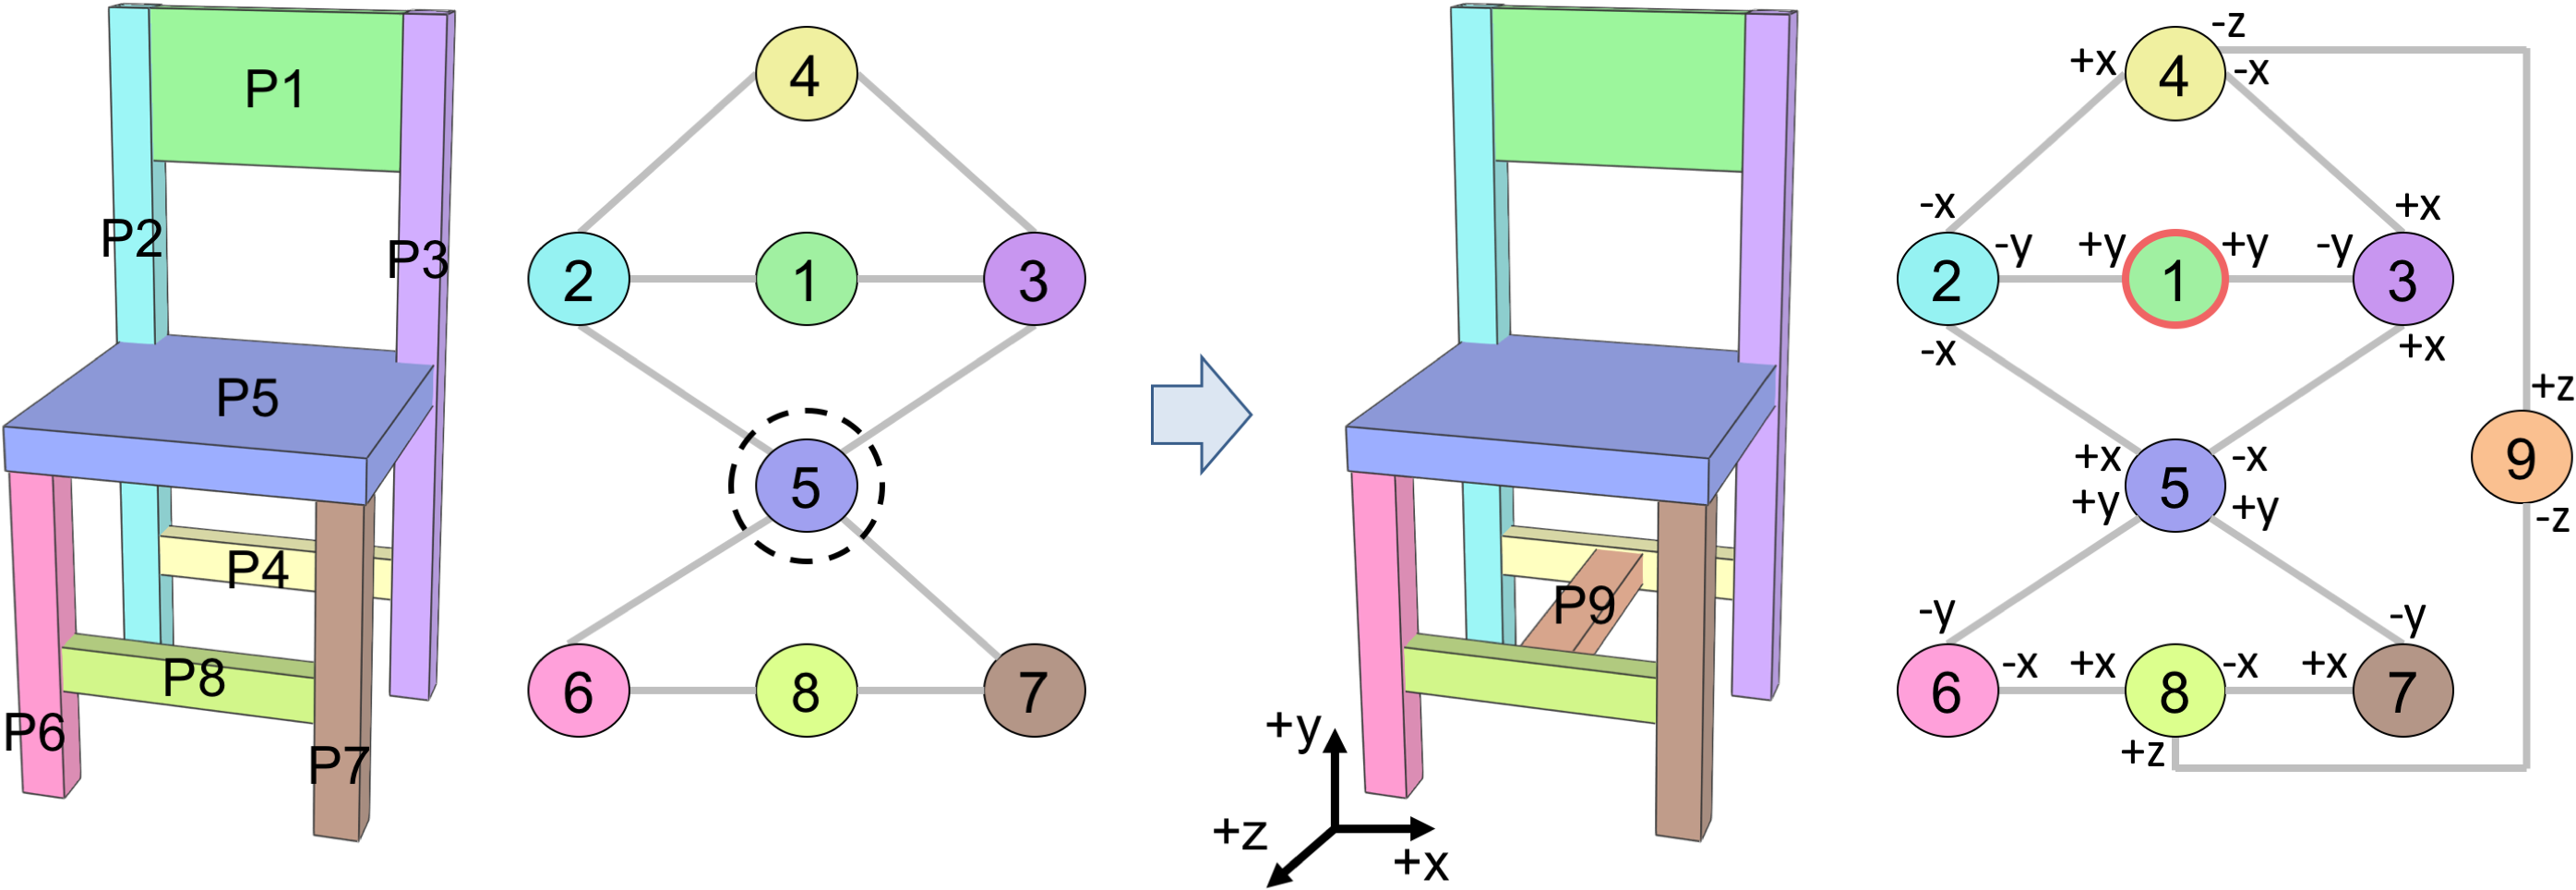
\includegraphics[width=8.45cm]{images/Result_Furniture_Chair.png}
	\vspace*{-2.5mm}
	\caption{
		Left: a {\textsc Chair} and its parts-graph, where a cut point (i.e., $P_5$) exists.
		Right: after adding a new part (i.e., $P_9$), our approach can generate an interlocking joint configuration, where the axial removal direction allowed by each joint is shown in the corresponding edge in the parts-graph. 
	}
	\vspace*{-4.5mm}
	\label{fig:Result_Furniture_Chair}
\end{figure}







\if 0
 Since our assembly supports non-orthogonal joints, we maintain a {\em dynamic set} of base DBGs denoted as $\{G(d, A_i)\}$ for each iteration of generating $\mathbf{A_i}$. The base directions of $\mathbf{A_i}$ are $\{d\} = \{d_1, ..., d_i\}$, where $d_j$ ($1 \leq  j \leq i$) is the removal direction of $P_j$.
Note that if $d_j = d_k$ ($j\neq k$, $d_j \in \{d\}$, $d_k \in \{d\}$), then $G(d_j, A_i)$ and $G(d_k, A_i)$ are actually the same DBG. For example, if all joint directions are axis-aligned as in Figure~\ref{fig:Application_Furniture_Table}, we end up with only three base DBGs.


Figures~\ref{fig:Application_Furniture_Table} and~\ref{fig:Application_Plate_Cabinet} show examples of interlocking plate structures. 

Figures~\ref{fig:Application_Furniture_Table}(g) shows the joint configuration planned by our approach, as well as geometry of each modified part.
Although both our approach and~\cite{Fu-2015-Furniture} can generate results on this input model, Section~\ref{sec:results} will show some of our results that cannot be achieved by~\cite{Fu-2015-Furniture}.


\fi




%%%%%%%%%%%%%%%%%%%%%%%%%%%%%%%%%%%%%%%%%%%%%%%%
% 3. Interlocking Frame Structures
%%%%%%%%%%%%%%%%%%%%%%%%%%%%%%%%%%%%%%%%%%%%%%%%

  \begin{figure*}[!t]
	\centering
	%\vspace*{-3.5mm}
	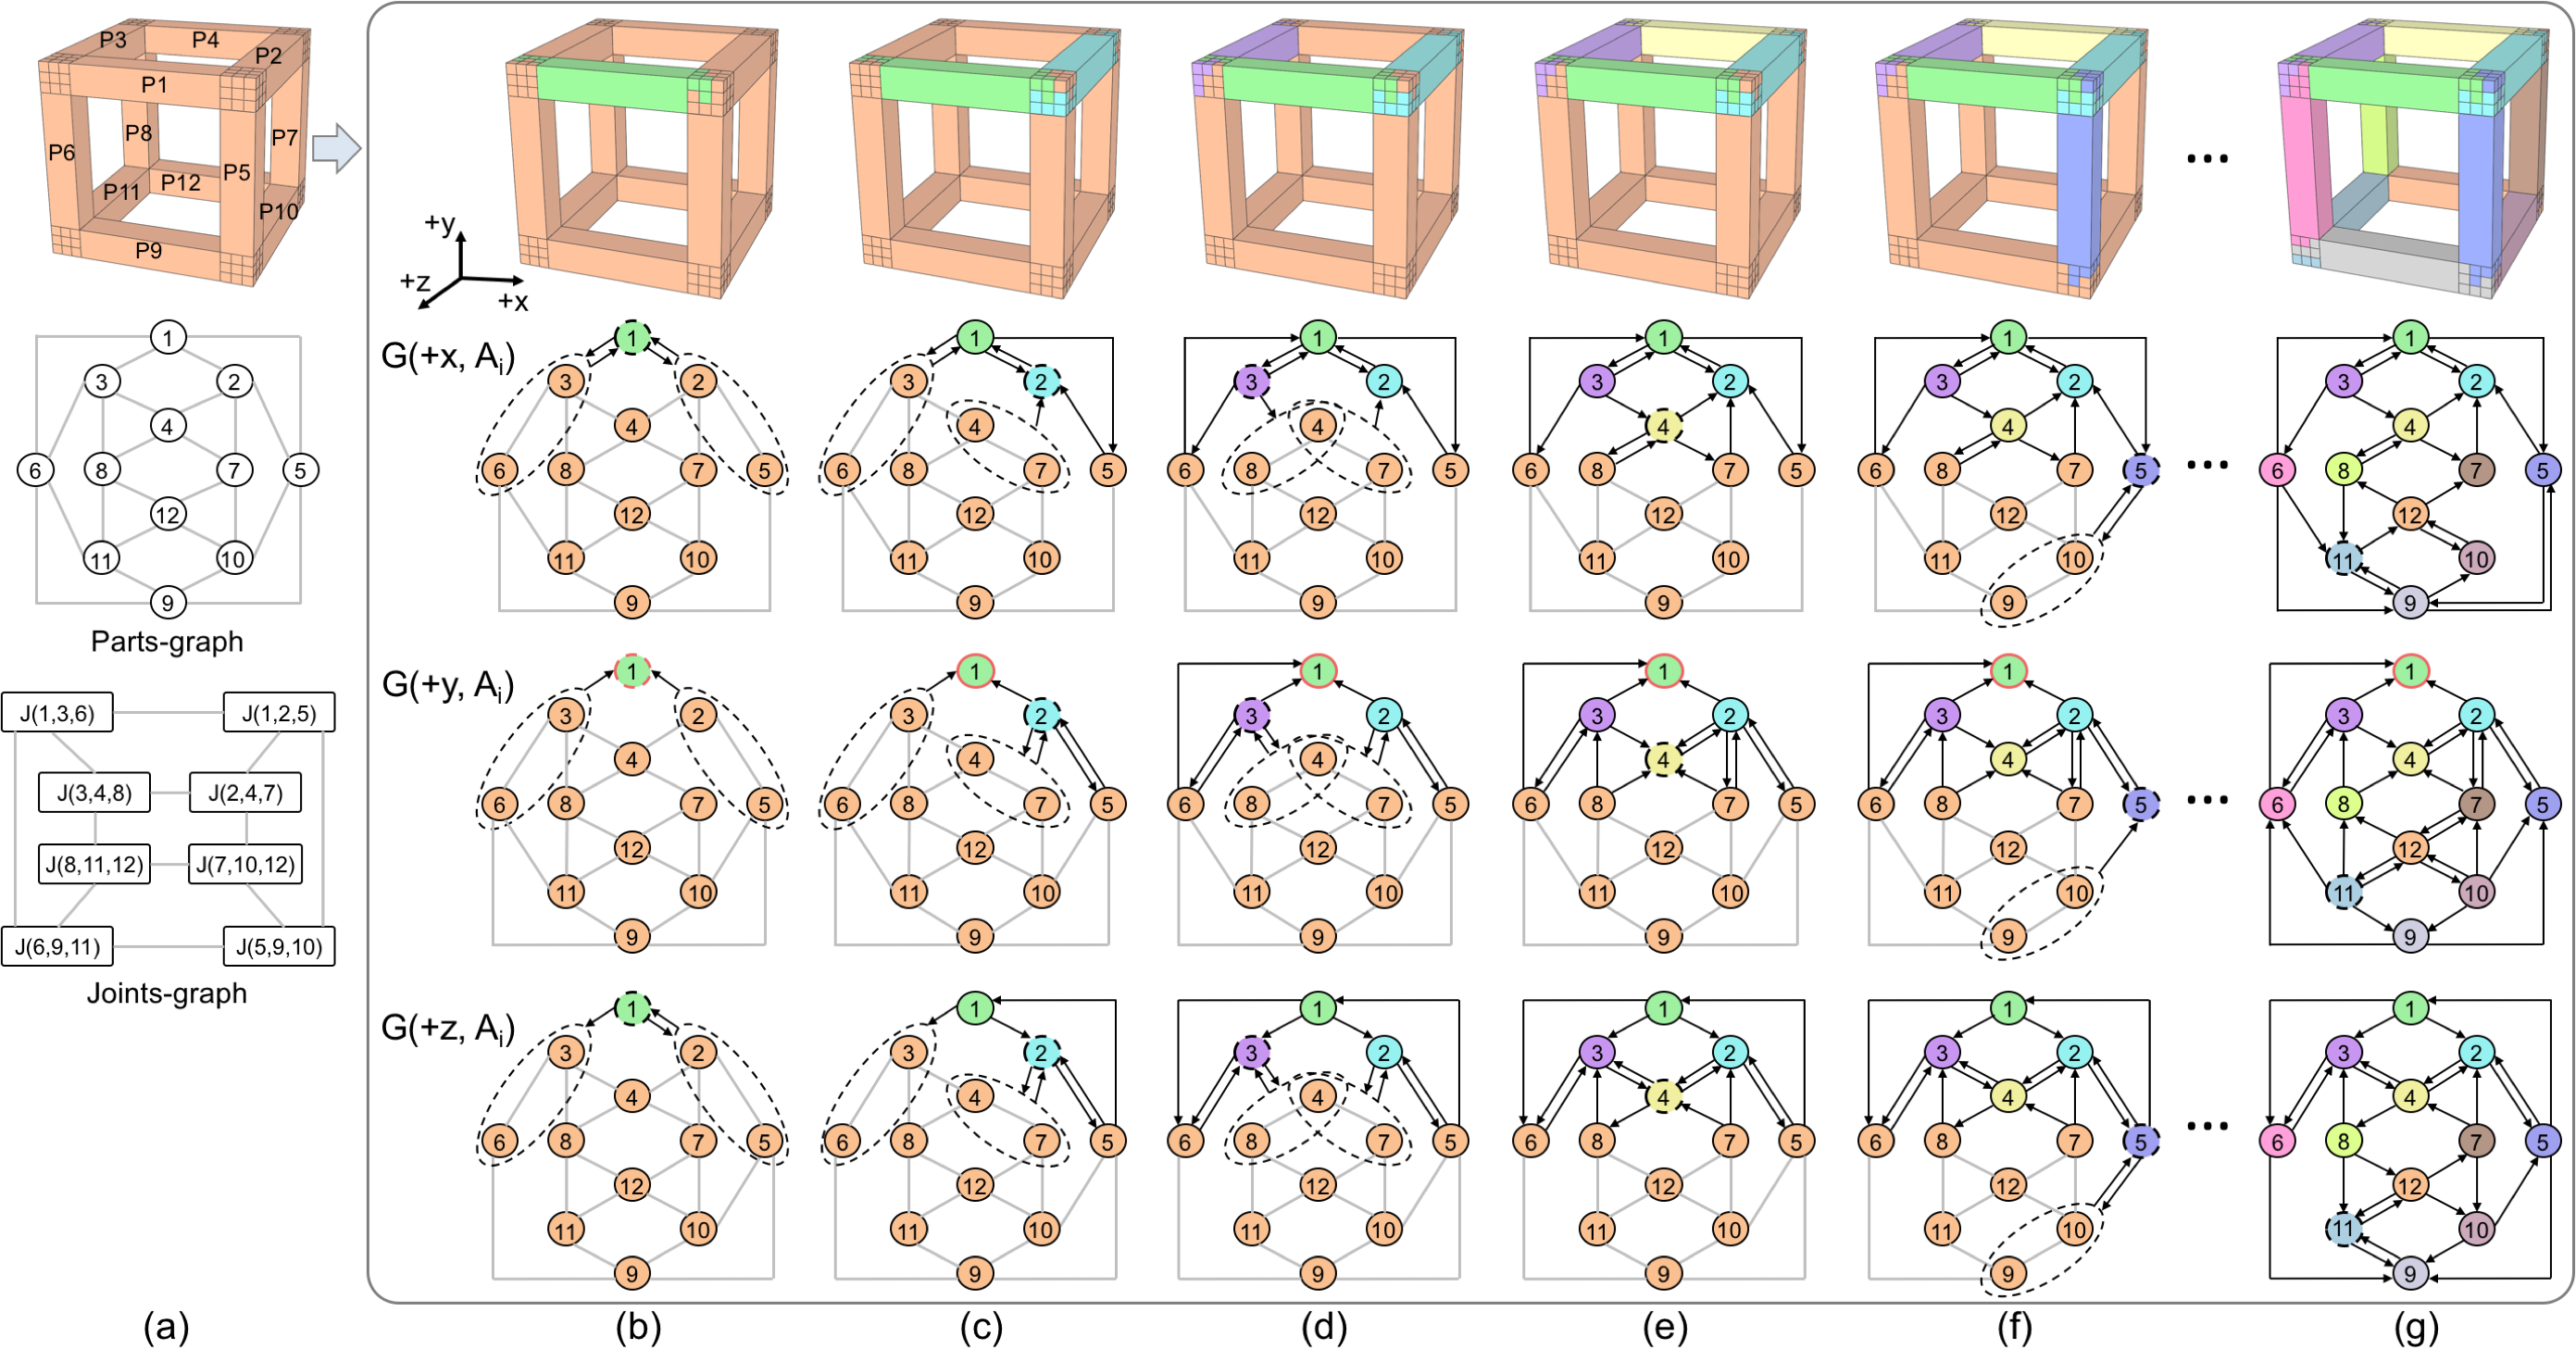
\includegraphics[width=17.75cm]{images/Application_Frame_Cube.png}
	\vspace*{-3.5mm}
	\caption{Design of a 12-part interlocking \textsc{Frame Cube}.
		(a) Input frame design, parts-graph, and joints-graph.
		(b-f) The iterative procedure to construct the cube joints, where the dashed ellipses highlight the set of parts in $R_i$ that connect with $P_j$ ($j\leq i$) using cube joints.
		% where all orange nodes in each DBG form $R_i$ and the node with dashed boundary is $P_i$.
		(g) The interlocking result.}
	\vspace*{-2.0mm}
	\label{fig:Application_Frame_Cube}
\end{figure*}



\subsection{Interlocking Frame Structures}
\label{subsec:frame}

% Problem formulation
As a new class of interlocking assembly, we propose  {\em interlocking frame structures} that can be considered a hybrid of the voxelized and the plate assemblies. A frame structure is a network of beams joined to represent a desired target shape. As input we assume a 3D polygonal mesh, where each edge represents a beam and each vertex represents a joint.
%Different from the furniture application, joint in a frame structure usually connects more than two parts, making traditional wooden joints infeasible.
%Thus, we propose to connect the beams with {\em puzzle joints}.
%Our goal is to construct a network of joints among all the beams to make the frame structure interlocking.

% Major different from furniture design
Compared with the plate assemblies, this application has two more challenges.
First, frame structures require connecting more than two parts at a joint, making traditional woodworking joints unsuitable; see the joints-graph in Figure~\ref{fig:Application_Frame_Cube}(a).
Thus, we propose to connect the beams with cube-shaped {\em voxel joints}.
To make the problem tractable, we assume that each face of the cube joint connects to at most one beam at the center voxel, and thus each cube connects at most six beams (i.e., valence of the input mesh should be at most 6).
Second, we need to individually optimize the geometry of each cube joint. We place an axis-aligned $3 \times 3 \times 3$ cube at each joint location and partition the cubes into pieces to restrict the relative movement of the connected beams; see the eight corners of the \textsc{Frame Cube} in Figure~\ref{fig:Application_Frame_Cube}(a). 
%
 % Customized framework
Compared to the plate structures, these specifics require the following adaptations to our framework:
%\vspace*{-2.0mm}
\begin{itemize}[leftmargin=*]
%	\item 
%	{\em Iterative Design Framework.} \	
%	The procedure is the same as that in Subsection~\ref{subsec:furniture}, except that we need to ensure geometric connectivity of each modified part.
%	To achieve this, we preassign the center voxel of the puzzle cube face to the part that is connected to that face.
%	Later, when we assign more voxels to the part at each of its two ends, we ensure that each group of assigned voxels (i.e., integral joint) are simply connected.
	
	\vspace*{1.0mm}
	\item 
	{\em Generating the key.} \
	For the cube joint at each end of $P_1$, we take the voxel preassigned to $P_1$ as a seed and include more voxels to $P_1$ such that it is movable along a singe axial direction following Subsection~\ref{subsec:genKey}.
	Denote the subset of parts that connect with $P_1$ at each end as $S_1^k = \{P_l\}$, where $k \in \{1, 2\}$; see the dashed circles in Figure~\ref{fig:Application_Frame_Cube}(b).
	After constructing $P_1$, we draw directed edges between $P_1$ and each $S_1^k$ in the DBGs accordingly.
	
	\vspace*{1.0mm}
	\item 
	{\em Generating $P_i$ and $R_i$ ($i>1$).} \
	%Denote the subset of parts that connect with $P_i$ at each end as $S_i^k = \{P_l\}$, where $k \in \{1, 2\}$.
	At the graph design stage, we classify parts in each $S_i^k$ into two groups: $\{ \grave{P}_l \}$ where each part is from $\{P_1, ..., P_{i-1} \}$ and $\{ \acute{P}_l\}$ where each part is from $R_i$. 
	If $\{ \acute{P}_l\}$ is empty, the blocking relations within this cube joint are completely defined.
	So the graph design of $P_i$ and $R_i$ can be skipped for this joint; see joint $J(1,2,5)$ in Figure~\ref{fig:Application_Frame_Cube}(f), where $P_i$ = $P_5$, $\{ \grave{P}_l \} = \{P_1, P_2\}$.
	If $\{ \grave{P}_l \}$ is empty, we do not need to distribute external blocking relations in this joint; see joint $J(2,4,7)$ in Figure~\ref{fig:Application_Frame_Cube}(c), where  $P_i$ = $P_2$, $\{ \acute{P}_l \} = \{P_4, P_7\}$.
	Otherwise, we distribute external blocking relations associated with $\{ \grave{P}_l \}$ to $P_i$ and parts in $\{ \acute{P}_l\}$ respectively; see joint $J(1,2,5)$ in Figure~\ref{fig:Application_Frame_Cube}(c).
	%, where $P_i$ = $P_2$, $\{ \grave{P}_l \} = \{P_1\}$,  $\{ \acute{P}_l\} = \{P_5\}$.
	Constructing internal blocking relations is restricted to $P_i$ and parts in $\{ \acute{P}_l\}$ for each $S_i^k$.
	To ensure that $P_i$ is disassemblable in $[P_i, R_i]$, say along $d_i$, we construct a single directed edge between $P_i$ and each part in $\{ \acute{P}_l\}$ for both $S_i^k$ in at least one DBG; see $G(+x, A_2)$ in Figure~\ref{fig:Application_Frame_Cube}(c) for an example.
%	The procedure to find candidates of $d_i$ and ensure interlocking of $\mathbf{A}_i$ conceptually is the same as that in Subsection~\ref{subsec:furniture}.

	%plan exactly the same joint between $P_i$ and each part in $R_i^{'}$; see Figure~\ref{fig:Application_Furniture_Table}(c\&e).
	%To ensure that $[P_1, ..., P_i, R_i]$ is interlocking, we try all possible $d_i$, and select those that result in at least one cycle including both $P_i$ and $R_i$ in each $G(d, A_i)$. 
	%Here, we find the candidates of $d_i$ by employing the joint analysis technique in~\cite{Fu-2015-Furniture}; e.g., the candidates of $d_1$ in Figure~\ref{fig:Application_Furniture_Table}(b) are $\{+x, -x, +y, +z, -z\}$.
	%For example, the candidates of $d_i$ in the inset are ${+x, -x}$. 
	%In particular, to ensure that the conceptual design is realizable in the embedded geometry, we employ the joint analysis technique in~\cite{Fu-2015-Furniture} to find the possible joints (and thus the associated axial direction) that can be deployed at the connection between $P_i$ and each part in $R_i^{'}$. 
	
	%\vspace*{1.0mm}
	%\item 
	%{\em Geometry Realization of $P_i$ and $R_i$.} \
	%Once we find an interlocking configuration (see Figure~\ref{fig:Application_Furniture_Table}(g)), 
	The geometry realization of $P_i$ and $R_i$ is conducted within the cube joint at each end of $P_i$ following the approach in Subsection~\ref{subsec:genPart}; see corners of the \textsc{Frame Cube} in Figure~\ref{fig:Application_Frame_Cube}(c-f).
	% which can be performed very efficiently since each puzzle joint has only 27 voxels.
\end{itemize}

\begin{figure}[!t]
	\centering
	%\vspace*{-3.5mm}
	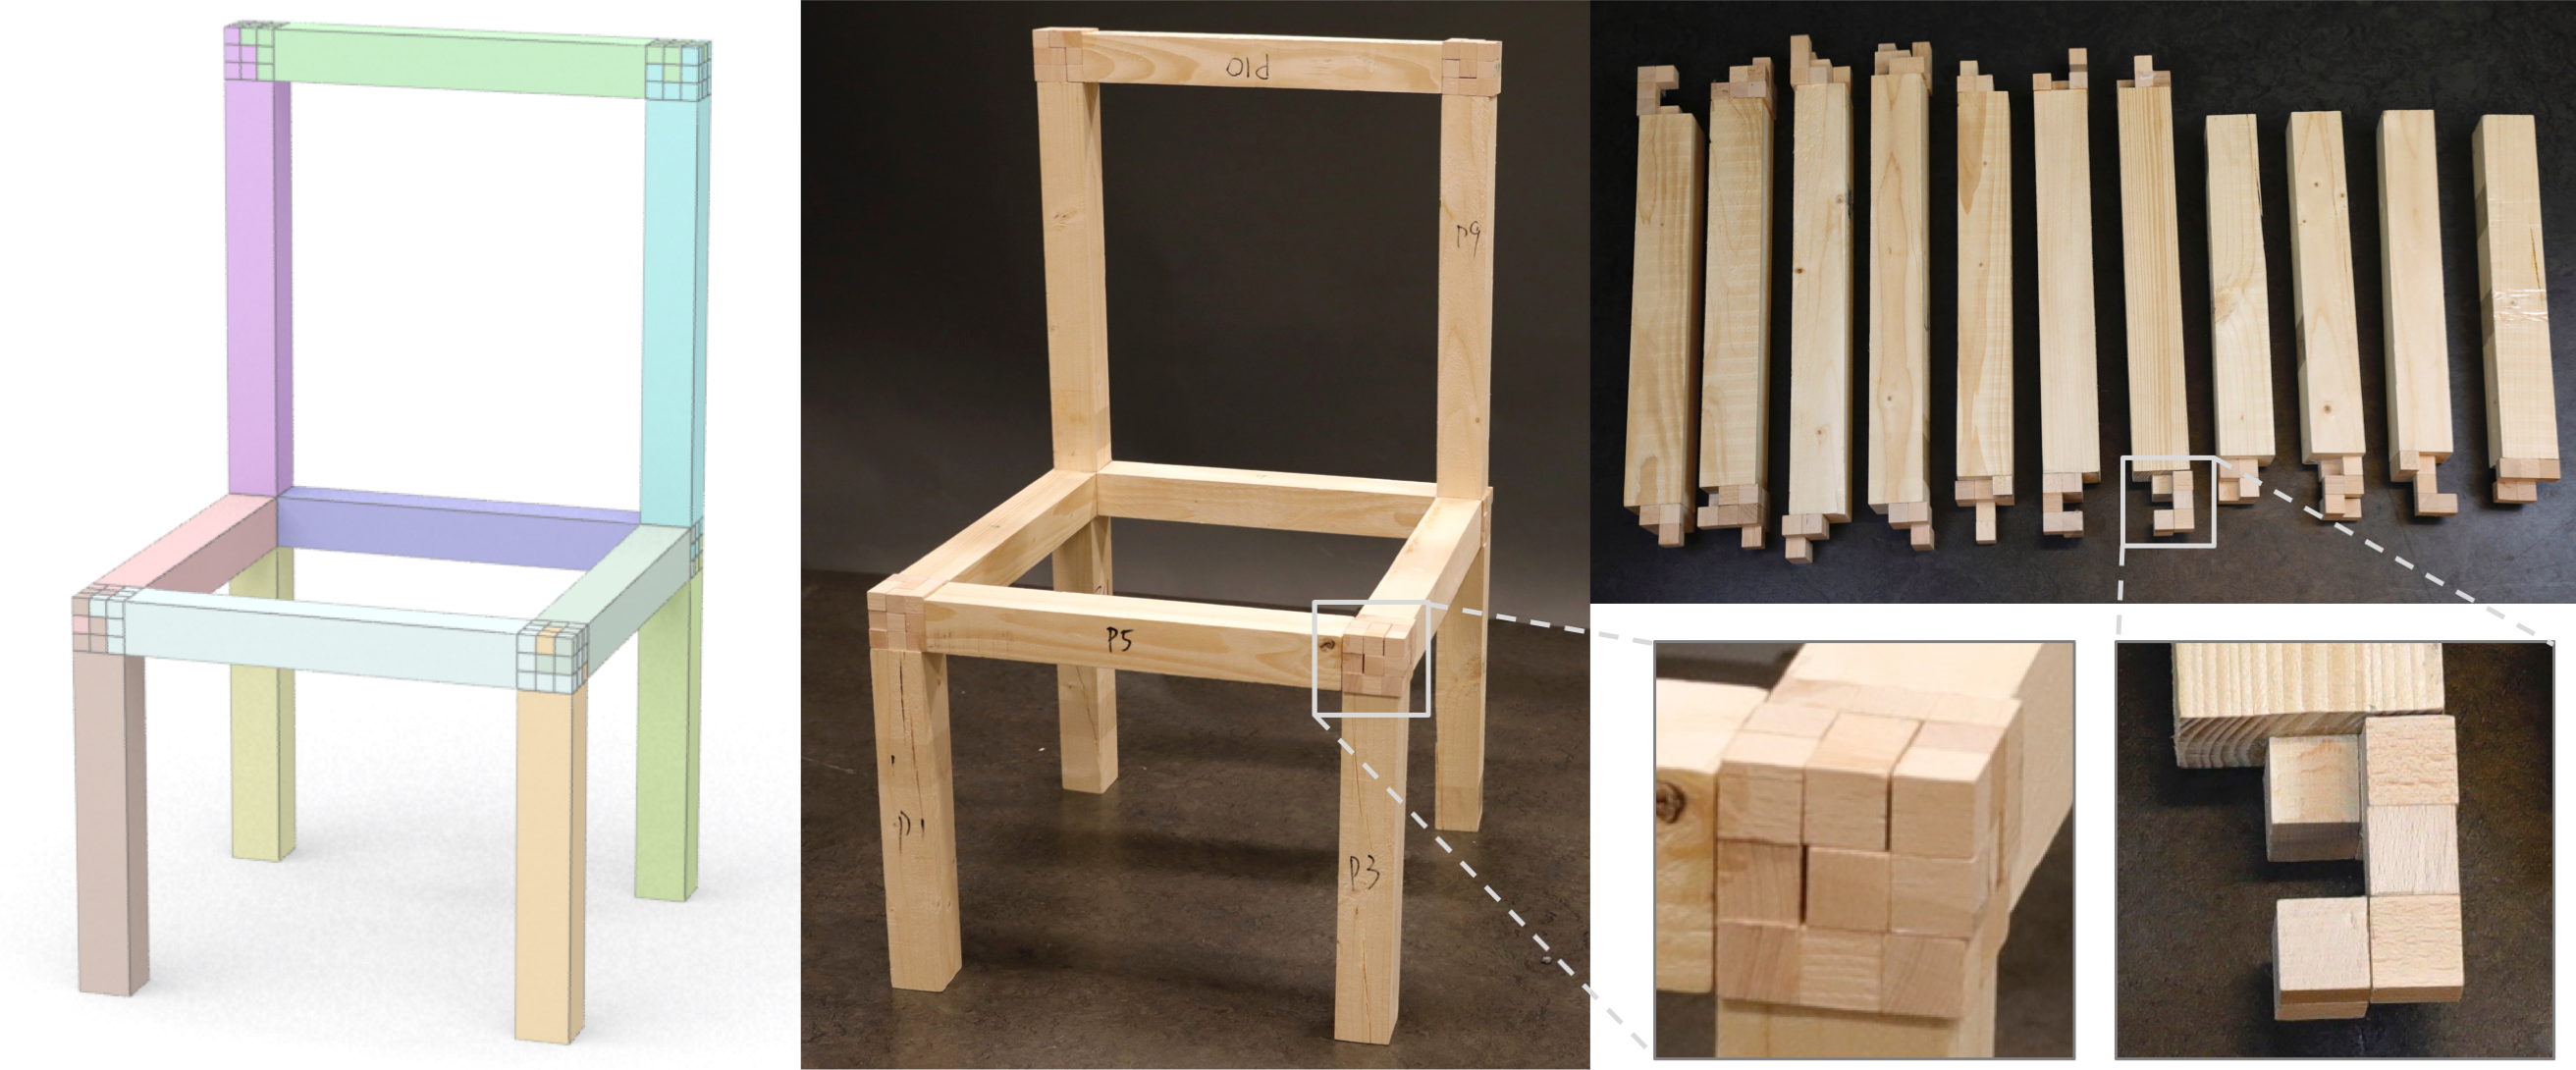
\includegraphics[width=8.45cm]{images/Result_Frame_Physical.png}
	\vspace*{-2.5mm}
	\caption{
		Interlocking $1.0m \times 0.5m \times 0.5m$ {\textsc Frame Chair}. The voxel joints are fabricated by gluing wooden cubes in the spatial arrangement computed by our algorithm. When attached to the corresponding wooden beams, all beams can be connected into a stable interlocking assembly.}
	\vspace*{-4.0mm}
	\label{fig:Result_Frame_Physical}
\end{figure}

Figure~\ref{fig:Application_Frame_Cube}(g) shows the resulting interlocking \textsc{Frame Cube}, in which every three beams joining at a corner are connected by a carefully constructed three-way cube joint. Note that all joints are distinct even though all corners are symmetric. This illustrates how the assembly order dictates the geometry of the joints, more so than the geometry of the parts.

Our approach can generate frame structures with different joint valence, e.g., the valence in the \textsc{Frame Chair} in Figure~\ref{fig:Result_Frame_Physical} can be 2, 3 or 4.
We fabricate this result using wooden pillars and small wooden cubes to validate its steadiness; see supplementary video for the live demo.
Figure~\ref{fig:teaser} shows another \textsc{Flower} result, where curved beams are connected by the cube joints to form an appealing structure.
%Note that the puzzle joints still have to be axial aligned in 3D space to satisfy the part surface contact requirement.
To the best of our knowledge, these are the first {\em single-key} interlocking frame structures.



% that connect beams with puzzle joints.


\subsection{Implementation and Performance}
% \TODO{Add some details of implementation, reference to source code, and some timing statistics.}
Our C++ implementation runs on an iMac with a 4.2GHz CPU and 32GB memory.
In general, the timing performance depends on the input model, the number of parts $N$, and additional design requirements.
Our approach creates interlocking plate structures very efficiently due to the relatively small search space.
For example, it takes 0.1 seconds to compute the \textsc{Cabinet} (Figure~\ref{fig:Application_Plate_Cabinet}), , 0.3 seconds for the \textsc{Bookshelf} (Figure~\ref{fig:teaser}), and  2.7 seconds for the \textsc{Lizard} (Figure~\ref{fig:teaser}).
Designing frame structures is also fast since the $3 \times 3 \times 3$ cubes that are optimized at each joint location have only 27 voxels.
The \textsc{Flower} (Figure~\ref{fig:teaser}) and \textsc{Frame Cube} (Figure~\ref{fig:Application_Frame_Cube}) take 4.1 and 0.8 seconds, respectively.
The computation time to create interlocking voxelized models highly depends on the number of desired parts. For example, the interlocking $4 \times 4 \times 4$ \textsc{Cube}s (Figure~\ref{fig:Application_Puzzle_Cube}) with 7, 8, and 9 parts take 0.3, 12, and 4,068 seconds respectively. For larger $N$ it becomes increasingly difficult to find an interlocking assembly, since smaller parts have fewer potential blocking contacts.
Enforcing additional design requirements can also increase the computation time substantially.
For example, creating the \textsc{Cartoon Dog} (Figure~\ref{fig:teaser}) without constraints takes 23.3 seconds, while incorporating the appearance constraints increases computation to 3,801 seconds, since significantly more backtracking is required to ensure that the constructed parts align with the features.
For more details on the implementation of our approach we refer to the source code provided in the supplementary material. 




%%%%%%%%%%%%%%%%%%%%%%%%%%%%%%%%%%%%%%%%%%%%%%%%
% 4. Interlocking Plate Structures
%%%%%%%%%%%%%%%%%%%%%%%%%%%%%%%%%%%%%%%%%%%%%%%%


%\subsection{Interlocking Plate Structures}
%\label{subsec:plate}
%
%% Problem formulation
%All above applications assume that the parts are orthogonally connected and are movable along axial directions.
%However, in our daily life there exist assemblies in which parts are non-orthogonally connected such as a bar stool with sloped legs.
%Our framework can be used to make such assemblies interlocking.
%Similar to the furniture application, our input is a plate structure design represented as a set of planar parts, and our goal is to make the design interlocking by constructing a network of joints between adjacent parts.
%
%% Joint models
%In this application, we consider the joint variants of halved-joint (HV) and mortise-and-tenon (MT), which allow parts to be non-orthogonally connected while contacting each other with planar surface; see Figure~\ref{fig:Application_Plate_Joints}.
%For a non-orthogonal HV joint, the removal direction is $\vec{e}$, which is an edge vector shared between parts.
%And we may choose between $+\vec{e}$ and $-\vec{e}$ when planning the joint; see Figure~\ref{fig:Application_Plate_Joints}(a\&b).
%For a non-orthogonal MT joint, the removal direction $\vec{d_t}$ of the tenon part is perpendicular to the part's normal; see Figure~\ref{fig:Application_Plate_Joints}(c\&d).
%


%
%
% % Customized framework
%Our framework is customized for designing plate structures, with following differences from the furniture application. 
%%\vspace*{-2.0mm}
%\begin{itemize}[leftmargin=*]
%	\item 
%	{\em Iterative Design Framework.} \	
%	The procedure is similar to that in Subsection~\ref{subsec:furniture},  except the base DBGs.
%	Rather than three base DBGs (for three axial directions), we maintain a {\em dynamic set} of base DBGs denoted as $\{G(d, A_i)\}$ for each iteration of generating $\mathbf{A_i}$. The base directions of $\mathbf{A_i}$ are $\{d\} = \{d_1, ..., d_i\}$, where $d_j$ ($1 \leq  j \leq i$) is the removal direction of $P_j$.
%	Note that if $d_j = d_k$ ($j\neq k$, $d_j \in \{d\}$, $d_k \in \{d\}$), $G(d_j, A_i)$ and $G(d_k, A_i)$ are actually the same DBG.
%	
%	\vspace*{1.0mm}
%	\item 
%	{\em Generate $P_1$ and $R_1$.} \
%	We select $P_1$ as the piece whose $\{\vec{e_i}\}$ has as many parallel directions as possible, and use this direction as $P_1$'s removal direction $d_1$ to facilitate joint construction on the key; see Figure~\ref{fig:Application_Plate_Cabinet}(b).
%	This is because we create a HV joint for the edge that is parallel to $d_1$, a MT joint for the edge that is nearly perpendicular to $d_1$ (angle within $[45^\circ, 135^\circ]$), and an empty joint for the other edges. 
%	
%
%	\vspace*{1.0mm}
%	\item 
%	{\em Generate $P_i$ and $R_i$ ($i>1$).} \
%	At the conceptual design stage, we need to select $d_i$ from $\{\vec{e_i}\}$ such that $\{G(d, A_i)\}$ satisfies the interlocking requirements, which can be classified into two cases.
%	
%	\vspace*{0.8mm}
%	The first case is that $d_i \in \{d_1, ..., d_{i-1} \}$, say $d_i = d_k$ ($1\leq k \leq i-1$).
%	For this case, each $G(d_j, A_i)$ ($j \neq k$) should satisfy the interlocking requirements automatically since the movement of $P_i$ along $d_i$ will not affect blocking relations for the other base directions.
%	Note that we avoid showing such graphs in Figure~\ref{fig:Application_Plate_Joints} to save space.
%	For $G(d_k, A_i)$, it inherits all blocking directions from $G(d_k, A_{i-1})$ and we add a single directed edge between $P_i$ and each part in $R_i$.
%	We try each of the two directions of the single edge and accept the conceptual design if $G(d_k, A_i)$ is strongly connected; see Figure~\ref{fig:Application_Plate_Cabinet}(g).
%	
%	\vspace*{0.8mm}
%	The second case is that  $d_i \notin \{d_1, ..., d_{i-1} \}$.
%	For this case, we build a new $G(d_i, A_i)$ by converting each undirected edge among $\{P_1, ..., P_{i-1}, R_{i-1}\}$ in the parts-graph into two directed edges and adding a single directed edge between $P_i$ and each part in $R_i$; compare Figure~\ref{fig:Application_Plate_Cabinet}(b\&c).
%	We try each of the two directions of the single edge and accept this conceptual design if $G(d_i, A_i)$ is strongly connected; see Figure~\ref{fig:Application_Plate_Cabinet}(c-f).
%	
%	%Among all valid conceptual designs, we rank  that results in a fewer number of empty joints.
%	Given a conceptual design, we create the joint geometry following the approach in Subsec~\ref{subsec:furniture}.
%	We rank the resulting candidates of $\mathbf{A}_i$ based on the total number of HV and MT joints.
%\end{itemize}
%

%Figure~\ref{fig:Application_Frame_Cube}(g) shows the resulting interlocking cube frame, in which every three beams joining at a corner are connected by a carefully constructed three-way puzzle joint.
%To the best of our knowledge, this is the first interlocking frame structure that connect beams with puzzle joints.



% Talk the difference with furniture
% Joints
% number of DBG
% part moving direction
% design aspect



%Story. \\
%1. motivation of this application, parts are non-orthogonally connected, part moving direction is not axis-aligned, but still require surface contact
%2. same as the furniture example, but the joints are tilted (show a image, compare with joints in CofiFab)
%Different from CofiFab since we need surface contact (mention advantage of it)
 %possible moving direction of each part (cross line of two planar parts) moving direction needs to be within the plane.
%3. classify based DBGs: 1) one that no part is movable; 2) one corresponding to the part moving direction
%4. when parts contact face are not parallel, it is easy to become interlocking but harder to be disassembled.
%5. base DBGs, the number of DBG increases dramatically; for each possible moving direction, 

%6. select one DBG corresponding to $d_i$ and try differetn $d_i$ and check whether it is strongly connected.
%select candidate based on the joints geometry






%%%%%%%%%%%%%%%%%%%%%%%%%%%%%%%%%%%%%%%%%%%%%%%%
% 1. Interlocking Puzzle
%%%%%%%%%%%%%%%%%%%%%%%%%%%%%%%%%%%%%%%%%%%%%%%%

\if 0
\Mark{1. Get user involved in the design process by using base DBGs, e.g., local blocking relations among certain parts;
	properties of the graphs such as more cycles  \\
	2. Prove the formal model of previous works~\cite{Song-2012-InterCubes, Fu-2015-Furniture} based on the graphs; \\
	3. Use base DGBs as an editing tool to allow users apply other design goals (e.g., pattern) into the design process; \\
	4. Make an existing non-interlocking assembly into an interlocking assembly: first build DBGs to analyze existing blocking relations;
	analyze the missing blocking relations; create geometry to realize the missing blocking relations \\
	5. Conceptual design does not consider the geometry; need to say sth about it in the paper.  \\
	6. Finalize the main story, list all the claims, and prepare all results to support the claims. \\ }



\vspace*{2.0mm}
\noindent
\TODO{list all claimed contributions and proposed experiments to support these claims}
\fi


%%%%%%%%%%%%%%%%%%%%%%%%%%%%%%%%%%%%%%%%%%%%%%%%%%%%%%%%%%%%%%%%%%%%%%%%%%%%%%%%%%%%%%%%%%%%%%%%%%%
% Backup
%%%%%%%%%%%%%%%%%%%%%%%%%%%%%%%%%%%%%%%%%%%%%%%%%%%%%%%%%%%%%%%%%%%%%%%%%%%%%%%%%%%%%%%%%%%%%%%%%%%









%%\input{supp-results.tex}
%%%%%%%%%%%%%%%%%%%%%%%%%%%%%%%%%%%%%%%%%%%%%%%%%%%%%%%%%%%%%%%%%%%%%
% Overivew
%%%%%%%%%%%%%%%%%%%%%%%%%%%%%%%%%%%%%%%%%%%%%%%%%%%%%%%%%%%%%%%%%%%%

\section{Conclusion}
\label{sec:conclusion}
\begin{figure}[!t]
	\centering
	%\vspace*{-3.5mm}
	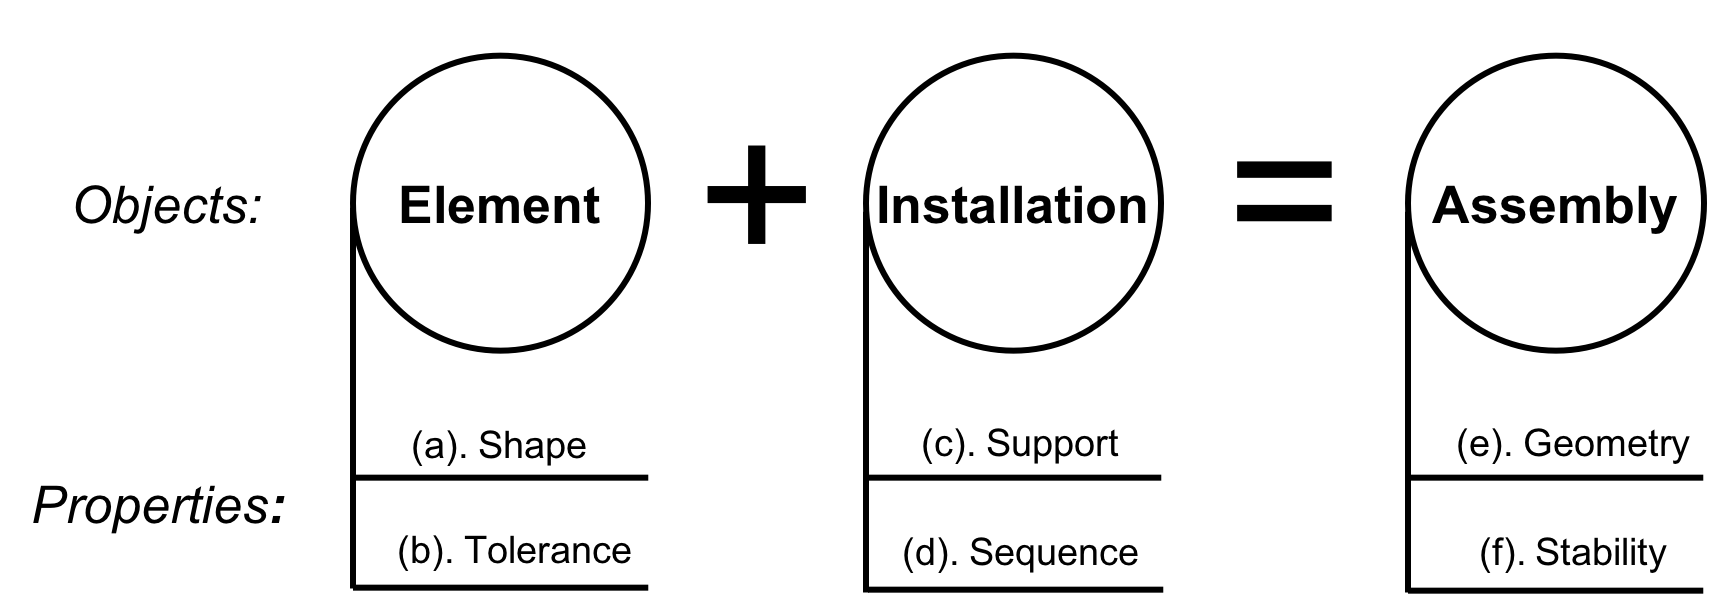
\includegraphics[width=8.00cm]{images/general_assembly.png}
	\vspace*{-2.5mm}
	\caption{The general framework of designing an assembly structure. The {\bf element} is the component part of the assembly and the {\bf installation} is the assembling process. (a) The feasible shape of element varies for different fabrication tools. For instance, 2D laser cutter only cuts 2D pattern on a flat plate but 3D printer could fabricate more freeform model. (b) Tolerance is the displacement between the fabrication and virtual model.  Machine cannot have infinite precision and the tolerance is inevitable during manufacture. (c) Temporary support such as scaffold stabilise the structure during assembling process. Less support could reduce the waste, which may takes up to 1/3 of the whole cost. (d) The assembling sequences includes the order of parts and the trajectory of placing the part in right positions. (e) User defined target geometry (f) Structural stability cares whether the whole structure will collapse under external load.
	}
	\vspace*{-4.0mm}
	\label{fig:general_assembly}
\end{figure}

This report takes a specific kind of assembly, the interlocking assembly, as an example. The interlocking property is formulated as a graph-based representation. Testing interlocking then is equivalent to analysing the strongly connected component of each DBG. The next step would be generating general interlocking structure with the help of DBGs.

However, it is better to consider more general topic beyond interlocking. The final goal of my PhD research is to build a general framework for assembly design. The composition of an general assembly includes six properties (see Fig. \ref{fig:general_assembly}). Among them, fabrication tolerance and structural stability are hard constraints and the reset have to optimize according to the demand. Besides, the framework also needs to maintain a sufficient design freedom for users. Considering all properties at same time is extremely challenging and most of the published work try to take a few properties into account. 

\vspace*{2mm}
\noindent
{\bf Properties (a) +  (d) + (e):} Most of the interlocking paper \cite{Song-2012-InterCubes},\cite{Xin-2011-BurrPuzzles}, \cite{Song-2016-CoFiFab}, \cite{Fu-2015-Furniture} are belong to this category. The constraints of installation sequence, where the key part is always the last pieces of the installation, is guaranteed by the element's shape. One of the common problem of these works is that without computing structural stability, the interlocking design is unsafe to be used in practice. Interlocking furniture, for instance, have three types of connections (see Fig.\ref{fig:Joints}). In practice, the structural strength of dovetail joint is weaker than the tenon joint. How to choose suitable joints according to the force flow while maintaining the interlocking property could be a promising research topic.
\begin{figure}[!t]
	\centering
	\vspace*{-4.0mm}
	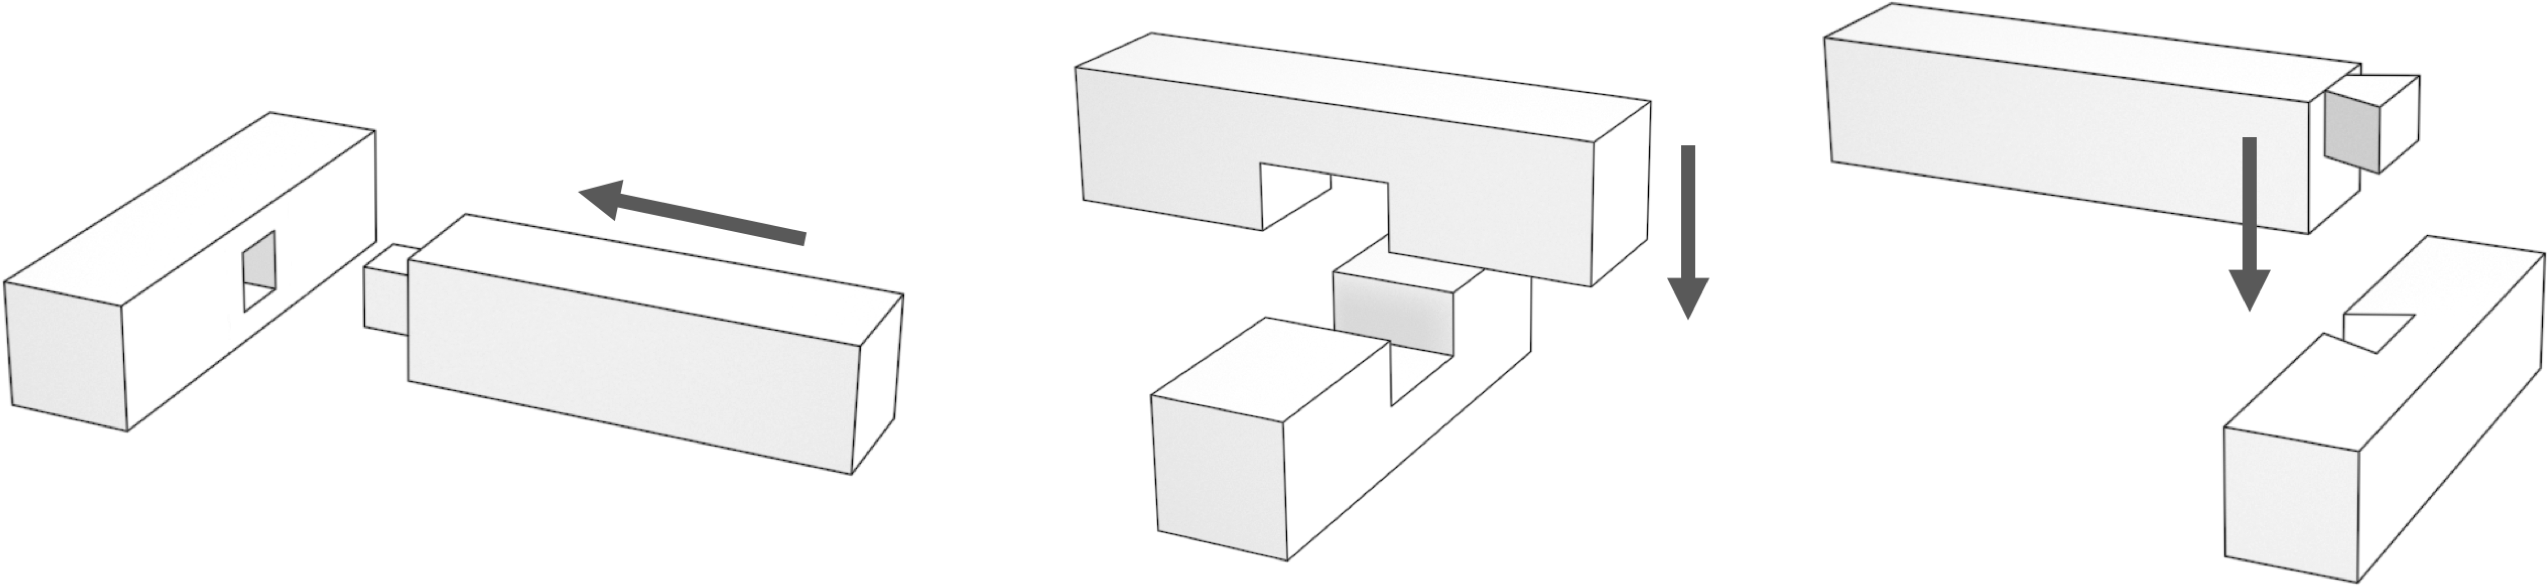
\includegraphics[width=8.00cm]{images/Joints.png}
	\vspace*{-2.5mm}
	\caption{Example woodworking joints. From left to right: mortise-and-tenon, halved joint, and dovetail joint, where the black arrow shows the single part movable direction allowed by the joint.}
	%\vspace*{-4.0mm}
	\label{fig:Joints}
\end{figure}

\vspace*{2mm}
\noindent
{\bf Properties (a) + (b) + (e):} Tolerance are usually required to accommodate the engineering error during manufacture, this resulted empty space allows each part of the assembly to have a small displacement. The accumulation of these displacements could be amplified greatly in a not well design and severely undermine the structure's stability (see Fig.\ref{fig:Gap_Issue}). A survey work of tolerance analysis is presented in \cite{chen2014comprehensive}. The tolerance analysis in mechanical engineering often deals with simple geometry and clear accumulation mechanism. However, our objects usually have complicated surface with ambiguous tolerance accumulation mechanism. One possible approach is to find the connection between the tolerance accumulation and cycles in DBGs. 
\begin{figure}[!b]
	\centering
	\vspace*{-3.0mm}
	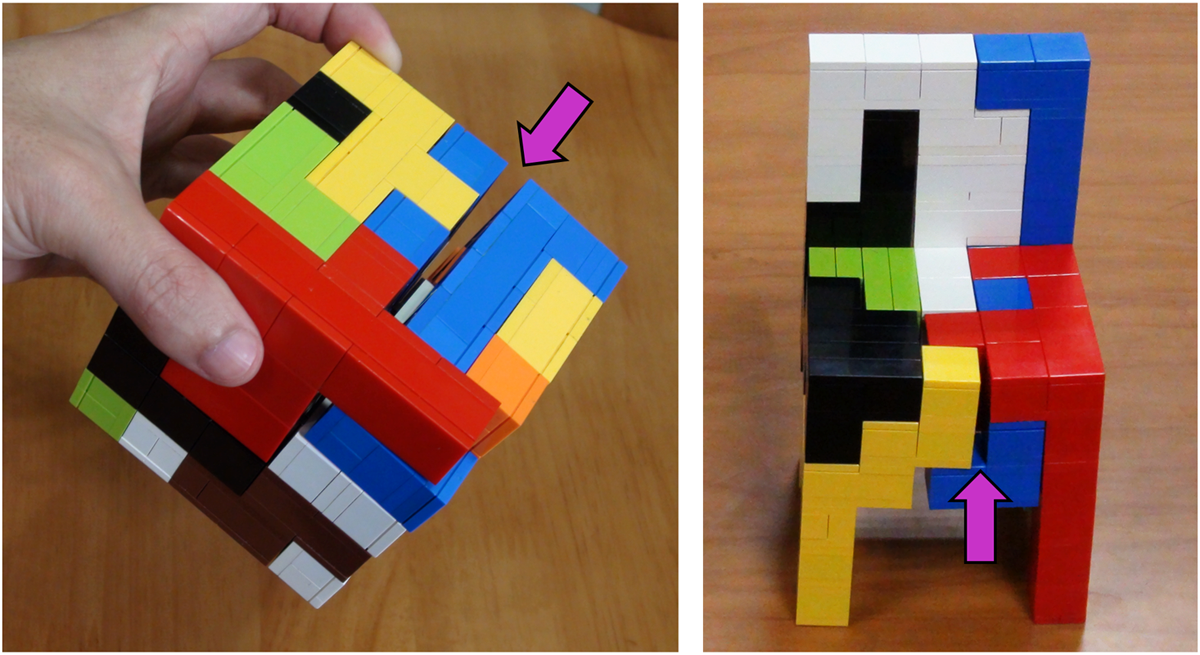
\includegraphics[width=8.30cm]{images/Gap_Issue.png}
	\vspace*{-1.0mm}
	\caption{Two  interlocking  puzzles  designed  by  implementing \cite{Song-2012-InterCubes}:  a  13-piece  cube  (left)  and  a  6-piece  chair  (right). Although being interlocking, both puzzles have the problematic gap issue (see arrows above) that loosens their structures. Note: LEGO bricks in fact have a tolerance of 0.20mm.
	}
	\vspace*{-4.5mm}
	\label{fig:Gap_Issue}
\end{figure}


%%%%%%%%%%%%%%%%%%%%%%%%%%%%%%%%%%%%%%%%%%%%%%%%%%%%%%%%%%%%%%%%%%%%%%%%%%%%%

%\bibliographystyle{ACM-Reference-Format}
%\bibliography{GeneralInterlock}
\end{document}


